\chapter{Fundamentos y conceptos básicos}
\label{capitulo:cap1}
\section{Algoritmo de la división}
Es usual ver una imagen como la siguiente (o semejante) cuando se calcula el cociente y el residuo de una división en la escuela. En la imagen, el cociente es 21 y el residuo 1.
\begin{figure}[h] 
    \centering
    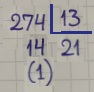
\includegraphics{divisionenpapel.jpg}
    \caption{Típica división escolar}
    \par\small Fuente: Elaboración propia
\end{figure}

El denominado Algoritmo de la División nos dice que tanto el cociente como el residuo son únicos.
\begin{enunciado}[Algoritmo de la División]\label{enun:algDivision}
\[\forall a,b \in \Z \text{ con } b \neq 0, 
\exists! q,r \in \Z \text{ tales  que }
a = q \cdot b + r \text{ donde } 0 \leq r < |b|\]
\end{enunciado}

\begin{proof}
Consideremos la progresión aritmética siguiente ($|b|$ es
la diferencia de la progresión):
\[ \ldots, a-3b, a-2b, a-1b, a+0b, a+1b, a+2b, a+3b, \ldots \]
De esta progresión seleccione el miembro \underline{no negativo menor} y denótelo como $r$. 
Siempre se puede expresar $r$ como $a-qb$ para algún $q \in \Z$.

En efecto, dado que todos los términos de la progresión son de la forma $a+kb$ con $k \in \Z$, siempre existe un entero $q$ tal que $r = a-qb$, basta tomar $q = -k$. 

Dado que se elige el miembro no negativo menor, es claro que: 
\begin{enumerate}[label=(\roman*)]
    \item $0 \leq r$.
    \item Mostraremos ahora que $r < |b|$, es decir, $r-|b| < 0$. 
\end{enumerate}

En efecto, supongamos que:
\begin{equation}
\label{eq35}
    r \geq |b|, \text{ es decir }, r -|b| \geq 0
\end{equation}
Como $r = a-qb$, entonces (\ref{eq35})  no es otra cosa que: $a-qb -|b| \geq 0$. 
O sea, por el valor absoluto, $a-qb - b \geq 0$ o $a-qb + b \geq 0$, que es lo mismo que:
\begin{equation}
    \label{eq41}
    a-(q+1)b \geq 0 \text{ o } a-(q-1)b \geq 0
\end{equation}
Pero entonces, no sólo $r - |b| \geq 0$, sino que, por la forma como se expresa esta desigualdad en (\ref{eq41}), $r - |b|$ es miembro de la progresión. 

Dado que $b \neq 0$, resulta que: 
\[|b| > 0 \qquad // \cdot(-1) \]
\[ -|b| < \, 0 \quad // +r \ \]
\[ r-|b| < \, r \]
Resumiendo: $r - |b| \geq 0$; $r - |b|$ miembro de la progresión; $r - |b| < r$. 

Ello contradice la elección de $r$ como el menor miembro no negativo.
Esta contradicción invalida nuestro supuesto, confirmando que
$r < |b|$. 

Falta probar la unicidad de $q,r$: 
Suponga que hay otro $r'$ tal que $r' = a-q'b$ con $0 \leq r' < |b|$. 
Es decir, $a = q'b + r'$ tal que $0 \leq r' < |b|$. 
Luego: $0 = a - a = qb + r - (q'b + r') = (q-q')b + (r-r')$.\\
Es decir: 
\begin{equation}
    \label{eq62}
    (r-r') = (q'-q)b
\end{equation}
Como $r'$ es un entero diferente de $r$, su diferencia no es cero, y por tanto, es claro que $q' \neq q$. Es decir $(q'-q) \neq 0$.
Luego (al trabajar en los enteros), el valor de $(q' - q)$ puede ser: 1 o -1 o 2 o -2 etc.
Es decir: $|q' - q| \geq 1$. Y como $b \neq 0$, de (\ref{eq62}) se deduce que: 
\begin{equation}
    \label{eq69}
    |r - r'| \geq |b|
\end{equation}
Pero ello contradice el hecho de que $0 \leq r < |b|$ y $0 \leq r' < |b|$. 

En efecto, tenemos: 
\[r < |b| \]  
\[r' \geq 0 \quad // \cdot(-1) \]
\[-r' \leq 0 \]
Luego:
$(r-r') < |b|$.
De modo análogo, tenemos: 
\[r \geq 0 \]
\[r' < |b| \quad // \cdot(-1)\]
\[ -r' > -|b| \]
Luego:
$(r-r') > -|b|$

Resumiendo: $(r-r') < |b|$ y $(r-r') > -|b|$\\
Recordemos que, por definición de valor absoluto, tenemos dos casos: 

Primer caso: $|r-r'| = r-r'$ cuando $r-r' \geq 0$. 
Como $(r-r') < |b|$, resulta que $|r-r'| < |b|$. 

Segundo caso: $|r-r'| = -(r-r')$ cuando $r-r' < 0$. Dado que 
\[(r-r') > -|b| \quad // \cdot(-1)\]
\[-(r-r') < |b| \]

Resultando que: $|r-r'| < |b|$. \\
En ambos casos: $|r-r'| < |b|$.

Así pues tenemos por un lado que $|r-r'| < |b|$  y por otro lado que (\ref{eq69}) $|r - r'| \geq |b|$. 

Dicha contradicción desahucia nuestro supuesto y confirma la unicidad de $q,r$. 
\end{proof}

\begin{itemize}
    \item $a,b$ se llaman respectivamente dividendo y divisor.
    \item $q,r$ se llaman respectivamente cociente y residuo de la división de $a$ entre $b$
\end{itemize}

Note que, dados $a,b$ la demostración ofrece un algoritmo para hallar los números $q,r$ a través de la progresión aritmética, el miembro no negativo menor y la forma de $r = a-qb$.

\begin{ejemplo}
Dados el dividendo $a = 5$ y el divisor $b = -2$, el cociente y el residuo son $q = -2$ y $r = 1$. \\
En efecto, la progresión es: \[
\ldots, 5-2\cdot (-2), 5-1\cdot (-2), 5+0\cdot (-2), 5+1\cdot (-2), 5+2\cdot (-2), 5+3\cdot (-2), \ldots \]
Es decir: \[
 \ldots, \qquad 9 \qquad, \qquad 7 \quad \quad, \qquad 5 \qquad, \qquad 3 \qquad, \qquad 1 \qquad, \qquad -1 \qquad,\ldots \]
El no negativo menor es $r = 1$. 
Todos los términos de la progresión son de la forma $a+kb$ con $k \in Z$, en el ejemplo el residuo 1 corresponde a $5+2\cdot (-2)$ con $k =  2$. Dado que en la demostración trabajamos con $r = a-qb$, tomamos $q = -k$, de donde se tiene que $q = -2$.
\end{ejemplo}

\section{Definiciones básicas}

\subsection{Divisibilidad}
\begin{definicion}[Divisibilidad]\label{def:divisibilidad}
Sean $a, b \in \Z$ con $b \neq 0$. 
Diremos que $b$ divide $a$ (o que $b$ es divisor o factor de $a$, o que $a$ es un múltiplo de $b$), denotado $b \mid a$, si $\exists q \in \Z$ tal que $a = qb$. Si $b<a$ se dice que es un divisor propio.
\end{definicion}

En relación con el algoritmo de la división, es evidente que $r = 0$ si y sólo si $b \mid a$. \\
Que $b$ no sea divisor de $a$ ($b$ no divide $a$) se denota así: $b \nmid a$.

\begin{ejemplo}
Con $a = 21$ y $b = 7$, tenemos que $b \mid a$ pues $21 = 3 \cdot 7$, con $q = 3$ y $r = 0$.
\end{ejemplo}

\begin{ejemplo}
Con $a = 20$ y $b = 6$, tenemos que $b \nmid a$ pues $20 = 3 \cdot 6 + 2$, con $q = 3$ y $r = 2$, es decir, $r \neq 0$.
\end{ejemplo}

\subsection{Máximo común divisor (mcd) y mínimo común múltiplo (mcm)}
\begin{definicion}[Divisor común]\label{def:divComun}
Dados $a,c \in \Z$, diremos que $d \in \Z$ es un divisor común de $a$ y $c$ si $d \mid a$ y $d \mid c$.
\end{definicion}

\begin{definicion}[mcd]\label{def:mcd}
Dados $a,c \in \Z$, no nulos ambos, diremos que $d \in \Z^{+}$ es el máximo cómún divisor de $a$ y $c$ si $d$ es el positivo mayor de los divisores comunes de $a$ y $c$. 
Se denota así: $mcd(a,c)$.
\end{definicion}

\begin{ejemplo}
El número 4 es divisor común de 24 y 36 pues $4 \mid 24$ \; y \; $4 \mid 36$.
\end{ejemplo}

\begin{ejemplo}
El número 12 es el máximo común divisor de 24 y 36, es decir, mcd(24,36) = 12, pues $12 \mid 24$ \; y \; $12 \mid 36$ y no hay otro divisor común positivo mayor a 12.
\end{ejemplo}

\begin{definicion}[mcm]\label{def:mcd}
El mcm (mínimo común múltiplo) de dos o más enteros $a_1, \ldots, a_r$ es el número positivo más pequeño que es múltiplo de todos ellos a la vez.  \\
Se denota así: $mcm(a_1, \ldots, a_r)$.
\end{definicion}

\begin{ejemplo}
El número $240$ es múltiplo común de $30, 40$ y $60$ pero no es el mínimo. \\
$mcm(30,40,60)=120$.
\end{ejemplo}

Tanto el $mcd$ como el $mcm$ son operaciones asociativas.

\subsection{Números primos y coprimos}

\begin{definicion}[Número primo]\label{def:numPrimo}
Un entero positivo $p > 1$ se llama número primo si sus únicos divisores positivos son 1 y $p$.
\end{definicion}

Un entero $n > 1$ no primo, se dice que es compuesto. 
El número 1 no es ni primo ni compuesto.

\begin{ejemplo}
Los números 3 y 5 son número primos pues sólo tienen a 1 y a sí mismos como divisores positivos.
\end{ejemplo}

\begin{ejemplo}
El número 6 es compuesto pues además de tener a 1 y 6 como divisores positivos, también $2 \mid 6$ \; y \; $3 \mid 6$.
\end{ejemplo}

\begin{definicion}[Números coprimos] \label{def:numCoprimo}
Dados $a,c \in \Z$, diremos que son coprimos (o primos entre sí o primos relativos) si $mcd(a,c) = 1$.
\end{definicion}

\begin{ejemplo}
Los números 4 y 9 son coprimos pues los divisores de 4 son 1, 2 y 4, los divisores de 9 son 1,3 y 9, de modo que mcd(4,9) = 1.
\end{ejemplo}

\subsection{Factor primo y factorización}
\begin{definicion}[Factor primo]\label{def:factorPprimo}
$\forall n \in \Z \; \ con \ n > 1, \text{un número primo} \ p$ se llama 
factor primo de $n$ si $p \mid n$.
\end{definicion}

\begin{definicion}[Factorización prima y multiplicidad]\label{def:factorizacion}
$\forall n \in \Z$ \; con $n > 1$, llamaremos factorización prima de $n$ a una expresión de la forma $n = p_1^{a_1} p_2^{a_2} \cdots p_k^{a_k}$, donde cada $p_i$ es un factor primo distinto y cada $a_i \in \N^{+}$.  El exponente $a_i$ se llama multiplicidad del factor primo $p_i$ en $n$, y representa la mayor potencia de $p_i$ tal que $p^{a_i} \mid n$.
\end{definicion}

Es usual denominar factorización al proceso de búsqueda de todos los factores primos junto a su multiplicidad.

\begin{ejemplo}
$n = 20$ tiene como factores primos a 2 y 5, pues $2|20$ y $5|20$. \\
La multiplicidad del factor primo 2 es 2, pues es el máximo exponente tal que $2^{2} \mid 20$. \\
La multiplicidad del factor primo 5 es 1, pues es el máximo exponente tal que $5^{1} \mid 20$ \\
La factorización de $20$ se expresa así: $20 = 2^{2} \cdot 5^{1} = 2^{2}5^{1}$.
\end{ejemplo}

\section{Propiedades de las definiciones básicas}
\subsection{Divisibilidad}
\begin{enunciado}[Propiedades de la divisibilidad]\label{enun:propDivisibilidad}\leavevmode\par
\begin{enumerate}[label=\roman*)]
\item Si $b \mid a$ \; y \; $b \mid c$ entonces $\forall x,y \in \Z$ \; $b \mid (ax + cy)$
\item Si $b \mid a$ \; y \; $a,b > 0$ entonces $b \leq a$
\item Si $b \mid a$ entonces $\forall x \in \Z$ \; $b \mid ax$
\item Si $a < b$ \; y \; $a,b > 0$ entonces $b \nmid a$
\item Si $c \mid b$ \; y \; $b \mid a$ entonces $c \mid a$
\item Si $b \mid (a+c)$ \; y \; $b \mid c$ entonces $b \mid a$
\end{enumerate}
\end{enunciado}

\begin{proof} Empecemos.
\begin{enumerate}[label=\roman*)]
\item Como $b \mid a$ \; y \; $b \mid c$ entonces $\exists q,q' \in \Z$ tales que $a = qb$ y $c = q'b$.
Luego: $ax + cy = qbx + q'by = (qx + q'y)b$. \\
Como $q,q',x,y \in \Z$, es obvio que $(qx + q'y) \in \Z$, entonces $b \mid (ax + cy)$. 
\item Como $b \mid a$ entonces $a = qb$. \\
Como $a,b > 0$, se deduce que $q > 0$, es decir, $q \geq 1$. \\
Por lo tanto: $qb \geq b$, es decir, $a \geq b$.  \label{inciso2}
\item Como $b \mid a$ entonces $a = qb$. \\
Luego: $ax = qbx = (qx)b$. \\
De lo cual, se desprende que $b \mid ax$. \\
\item Sabemos que $a,b >0$. \\
Supongamos que $b \mid a$. \\
Por el inciso \ref{inciso2} entonces $b \leq a$. Pero ello contradice $a<b$. \\
Por lo tanto, nuestro supuesto es errado y el enunciado se confirma. 
\item Como $c \mid b$ \; y \; $b \mid a$, resulta que $b = qc$ \; y \; $a = q'b$. Luego: \\
$a = q'b = q'qc = (q'q)c$. \\
De donde se deduce que $c \mid a$. 
\item Como $b \mid (a+c)$ \; y \; $b \mid c$ entonces $(a+c)=qb$ \; y \; $c=q'b$. Luego: \\
$(a+q'b) = qb$. Es decir: \\
$a = qb-q'b = (q-q')b$. \\
De donde se deduce que $b \mid a$.
\end{enumerate}
\end{proof}

\begin{ejemplo} Los incisos corresponden a los del enunciado. 
\begin{enumerate}[label=\roman*)]
\item Como $3 \mid 6$ \; y \; $3 \mid 15$ entonces $3 \mid (6 \cdot 3 + 15 \cdot (-7))$, es decir, $3 \mid -87$.
\item Como $2 \mid 4$ entonces $2 \leq 4$. 
Nótese que $-2 \mid -8$ pues $-8 = 4(-2)$. ¡Pero $-2 > -8$! \\
Ello no contradice el resultado pues, en este último caso, no es cierto que $a,b > 0$. 
\item Como $3 \mid 15$ entonces $3 \mid (15 \cdot (-1))$, es decir $3 \mid -15$.
Como $6 < 12$ \; y \; $6,12 > 0$ entonces $12 \nmid 6$.
\item Como $7 \mid 14$ \; y \; $14 \mid 28$ entonces $7 \mid 28$. 
\item Como $7 \mid (21+14)$ \; y \; $7 \mid 14$ entonces $7 \mid 21$.
\end{enumerate} \end{ejemplo}

\subsection{Máximo común divisor}
\begin{enunciado}[Propiedades del mcd]\label{enun:propMcd}\leavevmode\par
\begin{enumerate}[label=\roman*)]
\item Identidad de Bezout. Si $d = mcd(a,c)$ entonces  $\exists x,y \in \Z$ tales que $d = ax + cy$  
\item $mcd(-a,b) = mcd(a,b) = mcd(a,-b) = mcd(-a,-b) = mcd(|a|,|b|)$ 
\item $mcd(a,b) = mcd(b,a)$
\item Si $a,b \neq 0$ y $d = mcd(a,b)$ entonces $d \leq |a|$ y $d \leq |b|$
\item Para $a \neq 0, mcd(a,a) = |a|$
\item Para $b \neq 0, mcd(0,b) = mcd(b,0) = |b|$
\item Si $a,b > 0$ entonces $mcd(a,b) = mcd(b,r)$ \; \; ($r$ es el residuo de la división de a entre b) 
\item Lema de Euclides. Si $a \mid bc$ y $mcd(a,b) = 1$ entonces $a \mid c$
\item Una ecuación del tipo $ax + by = n$, se denomina ecuación diofántica. \\
La ecuación diofántica $ax + by = n$ tiene soluciones enteras
si y sólo si $mcd(a,b) \mid n$ 
\item Si $x_0,y_0$ es solución de la ecuación diofántica $ax + by = n$ entonces $\forall i$ tal que $i > 0$ $x' = x_0 + i \cdot \frac{b}{d}, y' = y_0 - i \cdot \frac{a}{d}$ también es solución
\end{enumerate} \end{enunciado}

\begin{proof} Empecemos. 
\begin{enumerate}[label=\roman*)]
\item Sea $S = \{ax + cy\}$ donde $x,y \in \Z$. \\
Escójanse $x_0,y_0$ tales que $b = ax_0 + cy_0$ sea el elemento positivo menor de S. \\
Por el algoritmo de la división,
\begin{equation} \label{eq273}
    \exists! q, r \in \mathbb{Z} \text{ tales que } a = qb + r, \text{ con } 0 \leq r < |b|
\end{equation}

Luego, $r = a-qb = a - q(ax_0 + cy_0) = a - qax_0 - qcy_0 = a(1 - qx_0) + c(-qy_0)$. 

Como $1,q,x_0,y_0 \in \Z$ es obvio que $(1 - qx_0), (-qy_0) \in \Z$. 

Por lo tanto, $r \in S$. 

Como $0 \leq r < |b|$ , es imposible que $0 < r$, pues el menor elemento positivo de S es b. 

Sólo queda la posibilidad $r = 0$. Y en ese caso, de (\ref{eq273}): $b \mid a$. 

Un razonamiento prácticamente idéntico 
($\exists! q,r \in \Z$ tales que $c = qb + r$) nos muestra que: $b \mid c$. 

Como $d$ es el máximo común divisor de $a$ y $c$, por definición: $d \mid a$ \, y \, $d \mid c$. 

Luego, por el Enunciado~\ref{enun:propDivisibilidad}.\roman{enumi}: 
$\forall x,y \in \Z \; \, d \mid (ax + cy)$. \\
En particular, $d \mid (ax_0 + cy_0)$. \\
Es decir: $d \mid b$, pues $b = ax_0 + cy_0$ \\
\setcounter{enumi}{2}
Por el Enunciado~\ref{enun:propDivisibilidad}.\roman{enumi}: $d \leq b$. \\
Por definición de máximo común divisor, d es positivo. \\
Por la forma de seleccionarlo, b es positivo. \\
Resumiendo: $b \mid a$ y $b \mid c$, $d \leq b$, $d$ es el máximo común divisor. \\
No nos queda sino concluir que $b = d$. \\
Es decir, $d = mcd(a,c) = ax_0 + cy_0$. Lo que prueba el enunciado. 
\setcounter{enumi}{1}
\item Mostraremos que $mcd(-a,b) = mcd(a,b)$ \\
Sea $d  =  mcd(-a,b)$. Es decir, $d \mid -a$ \, y \, $d \mid b$ (es el divisor común positivo más grande). \\
\setcounter{enumi}{3}
Por el Enunciado~\ref{enun:propDivisibilidad}.\roman{enumi}: $d \mid (-ax)$, tomemos $x = -1$, es decir, $d \mid a$.
Luego: $d \mid a$ y $d \mid b$. \\
No hay otro divisor positivo más grande. En efecto: \\
Supongamos que $d' \mid a$ \, y \, $d' \mid b$ con $d' > d$. De nuevo por el Enunciado~\ref{enun:propDivisibilidad}.\roman{enumi} con $x = -1$:
$d' \mid -a$ y $d' \mid b$, con $d' > d$, lo que contradice que $d  =  mcd(-a,b)$. \\
Por lo tanto: $d  =  mcd(a,b)$. \\
Los otros casos se prueban idénticamente, junto a la definición de valor absoluto en el último caso: 

$|a| = 
\begin{cases}
  a, & \text{si } a \geq 0, \\
  -a, & \text{si } a < 0.
\end{cases}$ 
\setcounter{enumi}{2}
\item Trivial. Por definición $d = mcd(a,b)$ es el divisor común positivo más grande de a y b. Luego, d es el positivo más grande tal que $d \mid a$ \, y \, $d \mid b$. Por tanto, d es el positivo más grande tal que $d \mid b$ \, y \, $d \mid a$.\\
Es decir, por definición, $d = mcd(b,a)$. 
\item  \setcounter{enumi}{2}
Por el inciso \roman{enumi}: $d = mcd(a,b) = mcd(|a|,|b|)$, es decir, $d \mid |a|$ \, y \, $d \mid |b|$. También $d > 0$ por definición. \\
Como $a,b \neq 0$: $|a| > 0$ \, y \, $|b| > 0$. Por el Enunciado~\ref{enun:propDivisibilidad}.\roman{enumi}: $d \leq |a|$ \,  y \, $d \leq |b|$. 
\setcounter{enumi}{4}
\item  
Sea $d = mcd(a,a)$. Por el inciso \roman{enumi}: $d \leq |a|$. \\
$|a|$ es divisor de $a$ pues $a = q|a|$, con $q = 1$ o $q = -1$. \\
Y como d es el máximo divisor, se concluye que $d = |a|$. 
\item \setcounter{enumi}{3} 
Por el inciso \roman{enumi}: Basta probar que para $b \neq 0, mcd(0,b) = |b|$. \\
\setcounter{enumi}{2}
Por el inciso \roman{enumi}: Es lo mismo probar que para $b \neq 0, mcd(0,|b|) = |b|$. \\
$|b|$ es divisor de $0$ pues: $0 = q|b|$ (con $q = 0$). \\
$|b|$ es divisor de $|b|$ pues: $|b| = q|b|$ (con $q = 1$). \\
Es decir, $|b|$ es divisor común de 0 y $|b|$. \\
No hay otro divisor común de 0 y $|b|$ más grande. En efecto:\\
Supongamos que lo hay. 

Sea d ese divisor común de 0 y $|b|$, con:
\begin{equation}
\label{eq343}
d > |b| 
\end{equation}


Como $b \neq 0: |b| > 0$ y por lo tanto $d > 0$. \\
Como $d$ es divisor de $|b|$ existe un $q$ talque
\begin{equation}
\label{eq351}
    |b| = qd
\end{equation}

Para que la última igualdad se mantenga (\ref{eq351}), dado que $|b|$,$d > 0$, se deduce que $q > 0$, es decir: 
\[
 q \geq 1 \quad // \cdot d
\]
\[
qd \geq d
\]
Luego, aplicando (\ref{eq351}): 
$|b| \geq d$. Lo que contradice la ecuación (\ref{eq343}). 

Así, nuestro supuesto es errado y $mcd(0,b) = |b|$. 
\setcounter{enumi}{6}
\item Por el Enunciado~\ref{enun:algDivision}: $a = qb + r$. Es decir: $r = a - qb$. \\
Sea $d = mcd(a,b)$ (es obvio que $d \mid a$ y $d \mid b$). \\
\setcounter{enumi}{1}
Por el Enunciado~\ref{enun:propDivisibilidad}.\roman{enumi}: $d \mid (a - qb)$. (con $x = 1, y = -q$). \\ Es decir, $d \mid r$ (y $d \mid b$). \\
No hay otro $d' > d$ tal que $d' \mid b$ y $d' \mid r$. En efecto: \\
Suponiendo que lo haya, por el mismo Enunciado~\ref{enun:propDivisibilidad}.\roman{enumi}: \\
$d' \mid (qb + r)$. \\
Es decir, $d' \mid a$, y como $d' \mid b$, se contradice el hecho de que $d = mcd(a,b)$. \\
Luego el supuesto es erróneo y $d = mcd(b,r) = mcd(a,b)$.
\setcounter{enumi}{7}
\item \setcounter{enumi}{1}
Como $mcd(a,b) = 1$, por el inciso \roman{enumi}: $1 = ax + by$. Luego: \\
$c = axc + byc$, es decir: $ c = acx + bcy$ \\
Es evidente que $a \mid ac$. \\
Por hipótesis sabemos que $a \mid (bc)$. Luego, por el Enunciado~\ref{enun:propDivisibilidad}.\roman{enumi}: \\
$ a \mid acx + bcy$. De donde se deduce que $a \mid c$.
\setcounter{enumi}{8}
\item Demostraremos el resultado, probando cada sentido de la doble implicación: \\
Sea $d=mcd(a,b)$.
\begin{enumerate}
\item Si la ecuación diofántica $a \cdot x+b \cdot y=n$ tiene soluciones enteras\\
entonces $mcd(a,b) \mid n$ :\\
Como $d=mcd(a,b)$ entonces: $d \mid a$ y $d \mid b$.\\
Entonces por el Enunciado~\ref{enun:propDivisibilidad}.i: $\forall x,y \in \Z: d \mid(a \cdot x+b \cdot y)$.\\
Por hipótesis existen $x_{0}, y_{0} \in \Z$ tales que $a \cdot x_{0}+b \cdot y_{0}=n$,\\
Por lo tanto: $d \mid n$.
\item Si $mcd(a, b) \mid n$ entonces\\
la ecuación diofántica $a \cdot x+b \cdot y=n$ tiene soluciones enteras:\\
Como $d=mcd(a,b)$, (por el inciso i): $\exists x_{0}, y_{0} \in \Z$ tales que $d=a \cdot x_{0}+b \cdot y_{0}$\\
Por hipótesis: $d \mid n$. Es decir: $\frac{n}{d} \in \Z$\\
Por lo tanto: $\frac{n}{d} \cdot x_{0} \in \Z, \frac{n}{d} \cdot y_{0} \in \Z$\\
Además ambos enteros solucionan la ecuación diofántica pues:\\
$a \cdot \frac{n}{d} \cdot x_{0}+b \cdot \frac{n}{d} \cdot y_{0}=\frac{n}{d} \cdot (a \cdot x_{0}+b \cdot y_{0})=\frac{n}{d} \cdot d=n$
\end{enumerate}
\setcounter{enumi}{9}
\item $a \cdot x'+b \cdot y'=a \cdot (x_{0}+i \cdot \frac{b}{d})+b \cdot(y_{0}-i \cdot \frac{a}{d})=a \cdot x_{0}+i \cdot a \cdot \frac{b}{d}+b \cdot y_{0}-i \cdot b \cdot \frac{a}{d}=a \cdot x_{0}+b \cdot y_{0}=n$
\end{enumerate}
\end{proof}

\begin{ejemplo} Los incisos corresponden a los del enunciado.
\begin{enumerate}[label=\roman*)]
\item $d = mcd(28,19) = 1$ \\
$\hspace*{0.8em}1 = 28(-2) + 19(3)$   con $x = -2, \, y = 3$. 
\item $mcd(12,18) = mcd(-12,18) = mcd(12,-18) = mcd(-12,-18) = 6$. 
\item $mcd(15,9) = mcd(9,15) = 3$. 
\item Con $a = -14, \, b = 35, mcd(-14,35) = 7, 7 \leq |-14| \, y \, 7 \leq |35|$. 
\item Con $a = -5, \, mcd(-5,-5) = 5 = |-5|$. 
\item Con $b = -12, \, mcd(-12,0) = mcd(-12,0) = 12 = |-12|$. 
\item Con $a = 56, \, b = 15, 56 = 15 \cdot 3 + 11$, donde $r = 11$. \\
$\hspace*{1.6em}mcd(56,15) = mcd(15,11) = 1$
\item Con $a = 5, \, b = 3, \, c = 10, bc = 30, 5 \mid 30, mcd(5,3) = 1, 5 \mid 10$.
\item  $4x + 6y = 10$ tiene solución pues $mcd(4,6) = 2$ y $2 \mid 10$; $x_0=1, y_0=1$ solucionan esta ecuación diofántica.
\item Dada la solución $x_0=1, y_0=1$ para $4x + 6y = 10$, con $i=1$, $x'=1+1 \cdot \frac{6}{2}=4, y'=1-1 \cdot \frac{4}{2}=-1$ también es solución.
\end{enumerate}
\end{ejemplo}

\subsection{Divisores primos y teorema fundamental de la aritmética}
\begin{enunciado}[Propiedades de un divisor primo]\label{enun:propDivprim}
\leavevmode\par
\begin{enumerate}[label=\roman*)]
\item Sea $p$ primo. $\forall a \in \Z$ \, se tiene $p \mid a$ \, o \, $mcd(a,p) = 1$ 
\item Sea $p$ primo. $\forall a,b \in \Z$ \; Si $p \mid ab$ entonces $p \mid a$  \, o  \, $p \mid b$
\item Generalización del Lema de Euclides. Sea $p$ primo. $\forall a_1, \ldots, a_k \in \Z$  \; Si $p \mid (a_1 \cdot \ldots \cdot a_k)$ entonces $\exists i$, con $1 \leq i \leq k$, tal que $p \mid a_i$
\end{enumerate}
\end{enunciado}

\begin{proof} Empecemos.
\begin{enumerate}[label=\roman*)]
\item Sea $d = mcd(a,p)$. \\
Dado que $p$ es primo sus únicos divisores son $1$ y $p$, luego $d = 1$ o $d = p$. \\
Si $d = 1$, entonces $mcd(a,p) = 1$. \\
Si $d = p$, como $d \mid a$ entonces $p \mid a$. \\
En ambos casos, se cumple $p \mid a$ \, o \, $mcd(a,p) = 1$. 
\item Si $p \mid a$ el resultado es cierto inmediatamente. \\
Supongamos que $p \nmid a$. \\
Como $p$ es primo, sus únicos divisores son $1$ y $p$, de modo que el único divisor común positivo entre $a$ y $p$ es $1$ (el otro candidato es $p$, pero al no ser divisor de a, se descarta). Luego, $mcd(a,p) = 1$. \\ 
Por el Enunciado~\ref{enun:propMcd}, concretamente el Lema de Euclides, $p \mid b$. \\
Ello prueba que o bien $p \mid a$ \, o \, $p \mid b$. 
\item Como $p \mid (a_1 \cdot \ldots \cdot a_k)$ es obvio que $p \mid (a_1 \cdot (a_2 \cdot \ldots \cdot a_k))$. \\
\setcounter{enumi}{2}
Por el inciso \roman{enumi}: $p \mid a_1$ o $p \mid (a_2 \cdot \ldots \cdot a_k)$. \\
Si $p \mid a_1$ el resultado es cierto inmediatamente. \\
Si $p \mid (a_2 \cdot \ldots \cdot a_k)$ entonces $p \mid (a_2 \cdot (a_3 \cdot \ldots \cdot a_k))$. Etc. \\
Es un corolario del inciso \roman{enumi}.
\end{enumerate}
\end{proof}

\begin{ejemplo} Los incisos corresponden a los del enunciado. \\
\begin{enumerate}[label=\roman*)]
\item Con $p = 7$, \, $a = 14, 7 \mid 14$. Se cumple que $p \mid a$.\\
\hspace*{1em} Con $p = 7, \, a = 15, \, mcd(7,15) = 1$. Se cumple que $mcd(a,p) = 1$.
\item Con $p = 5, a = 10, b = 3, 10 \cdot 3 = 30, 5 \mid 30, 5 \mid 10$. Se cumple que $p \mid a$. \\
\hspace*{1em} Con $p = 3, a = 7, b = 12, 7 \cdot 12 = 84, 3 \mid 84, 3 \mid 12$. Se cumple que $p \mid b$.
\item Con $p = 11, a_1 = 4, a_2 = 11, a_3 = 9, a_4 = 5, a_5 = 2, 4 \cdot 11 \cdot 9 \cdot 5 \cdot 2 = 3960, 11 \mid 3960$ \\  \hspace*{1.2em} $\exists i, i = 2$, tal que $11 \mid a_2$. 
\end{enumerate}
\end{ejemplo}

\begin{enunciado}[Teorema fundamental de la aritmética (factorización única)]\label{enun:teorFundAritm}
$\forall n \in \Z$ \; con $n > 1$, (salvo el orden de los factores)  existe una única factorización prima de $n$, es decir, una única expresión de la forma $n = p_1^{a_1} p_2^{a_2} \cdots p_k^{a_k}$.
\end{enunciado}

\begin{proof} Si $n$ es primo, por sí solo se considera como el producto de un único factor. \\ 
En otro caso, designemos por $p_1$ a su divisor primo menor, luego (por definición de divisor): $n = p_1n_1$. 
\begin{itemize}
    \item Si $n_1 > 1$, designemos por $p_2$ a su divisor primo menor, luego:  $n_1= p_2 n_2$.
    \item Si $n_2 > 1$, designemos por $p_3$ a su divisor primo menor, luego:  $n_2 = p_3 n_3$. 
    \item Hasta que obtengamos un $n_r = 1$, de manera que $n_{r-1} = p_r$.
\end{itemize}

En efecto, este proceso de escribir n como el producto de sus factores primos debe terminar porque los factores son menores que n y además cada factor primo es un entero mayor que $1$. 

Reemplazando $n_1$ en la primera igualdad por $p_2 n_2$, y luego reemplazando $n_2$ en el resultado, y así sucesivamente, $n$ puede expresarse como el producto de estos factores primos hallados como hemos indicado: $n = p_1 p_2 \cdots p_{r-1} p_r$ 
Y como los factores primos no son necesariamente distintos podemos escribir: 

$n = p_1^{a_1} p_2^{a_2} \cdots p_k^{a_k}$, donde $p_1, p_2, \cdots, p_k$ son primos distintos y $a_1, a_2, \cdots, a_k$ son positivos. 

Es el turno de la \underline{unicidad}: 

Supongamos que hay enteros positivos con más de una factorización. Sea $n$ (con $n > 1$) el menor de ellos. 

Nótese que estamos llamando factorización (y no factorización prima) a la expresión que contiene factores primos duplicados, todavía sin unificarlos a través de los exponentes $a_i$.

Como para $n$ hay otra factorización, sea dicha factorización alterna la siguiente: 
\begin{equation}
\label{eq1}
n = q_1 q_2 \cdots q_{s-1} q_s
\end{equation}
Luego: $p_1 p_2 \cdots p_{r-1} p_r = q_1 q_2 \cdots q_{s-1} q_s$\\ 
Es claro que $q_1 \mid q_1 q_2 \cdots q_{s-1} q_s$. Luego: \\ 
$q_1 \mid p_1 p_2 \cdots p_{r-1} p_r$ (es decir: $q_1 \mid n$). \\
\setcounter{enumi}{3}
Por el Enunciado~\ref{enun:propDivprim}.\roman{enumi}: $q_1$ es divisor de al menos uno de los $p_i$. \\ 
Podemos suponer (reordenando los factores primos si es necesario) que $q_1 \mid p_1$. \\ 
Pero $p_1$ y $q_1$ son primos, luego, necesariamente: $p_1 = q_1$.    (luego:  $p_1 \mid n$) \\ 
Simplificando (\ref{eq1}) por $p_1 = q_1$ tenemos que: 
\begin{equation}
\label{eq481}
m = n/p_1 = 1 p_2 \cdots p_r-1 p_r =  q_2 \cdots q_{s-1}  q_s
\end{equation}
Como $p_1 \mid n$, entonces $m$ es un entero positivo. Además: $m < n$. \\ 
Pero entonces, (\ref{eq481}) nos muestra que $m$ tiene más de una factorización. \\ 
Lo que contradice que $n$ sea el menor de los enteros positivos con más de una factorización. \\ 
De ahí que nuestro supuesto es erróneo y la factorización es única.
\end{proof}

\begin{ejemplo} Trabajemos con $n = 252$. \\
Factorización (como en la demostración): \\
El menor primo que divide a 252 es 2. \\
$252 = 2 \cdot 126$. \\
El menor primo que divide a 126 es 2. $126 = 2 \cdot 63$. Luego: \\
$252 = 2 \cdot 2 \cdot 63$. \\
El menor primo que divide a 63 es 3. $63 = 3 \cdot 21$. Luego: \\
$252 = 2 \cdot 2 \cdot 3 \cdot 21$. \\
El menor primo que divide a 21 es 3. $21 = 3 \cdot 7$. Luego: \\
$252 = 2 \cdot 2 \cdot 3 \cdot 3 \cdot 7$. \\
El menor primo que divide a 7 es 7. $7 = 7 \cdot 1$. \\
Hemos obtenido un $n_r = 1$, de manera que $n_{r-1} = p_r = 7$. Luego: \\
$n = p_1 p_2 \cdots p_{r-1} p_r$. Es decir: \\ 
$252 = 2 \cdot 2 \cdot 3 \cdot 3 \cdot 7$. \\ \\
Factorización prima de $n = 252$, con  $a_1 = 2, a_2 = 2, a_3 = a_k = 1$ : \\
$252 = 2^{2} \cdot 3^{2} \cdot 7^{1} = 2^{2} \cdot 3^{2} \cdot 7 $.
\end{ejemplo}

\begin{enunciado}[Infinitud de primos]\label{enun:infPrim} Existen infinitos números primos.
\end{enunciado}

\begin{proof} Por reducción al absurdo. \\
Supongamos que sólo hay $n$ número primos. \\
Listémoslos en forma creciente así: $p_1, p_2, \cdots, p_n$. \\
Sea $N = p_1 p_2 \cdots p_{n-1} p_n + 1$. De donde, $N - p_1 p_2 \cdots p_{n-1} p_n = 1$. \\
Por el teorema fundamental de la aritmética, Enunciado~\ref{enun:teorFundAritm}, existe una factorización prima única de $N$. Es decir, $N$ es un producto de primos, llamemos $p_j$ a uno de ellos.  Otra forma de decirlo es que $N$ tiene al menos un divisor primo $p_j$. Es decir: $p_j \mid N$. \\
También es obvio que $p_j \mid p_1 p_2 \cdots p_n$. \\
\setcounter{enumi}{1}
Por el Enunciado~\ref{enun:propDivisibilidad}.\roman{enumi}: $p_j \mid (N - p_1 p_2 \cdots p_n)$, con $x = 1, y = -1$. Es decir: $p_j \mid 1$. \\
Ello implica que $p_j = 1$. Lo que contradice que $p_j$ es primo. \\
De ahí que nuestro supuesto es erróneo y no hay un número finito $n$ de números primos.
\end{proof}

\section{Estructuras modulares y congruencia}
La palabra módulo tiene varios significados en matemática (por ejemplo es un sinónimo de valor absoluto).
Nos interesan los siguientes dos: el primero relacionado con el residuo, en tanto operación, y el segundo relacionado con la relación de congruencia.

\subsection{Módulo como operación}
$a \bmod b = r$ \; ($r$ es el residuo de la división de $a$ entre $b$). \\

\begin{ejemplo} $19 \bmod 17 = 2$ pues en la división de $a$ entre $b$, con $a = 19, b = 17$, el residuo $r = 2$. \\ En efecto, $19 = 1 \cdot 17 + 2$
\end{ejemplo}

\subsection{Módulo como base de la (relación de) congruencia}
Sea $n \in \N$. Sean $a,b \in \Z$. \\
Se dice que $a$ es congruente con $b$ módulo $n$ (o también $a,b$ son congruentes módulo $n$), lo que se denota así: $a \equiv b \pmod n$ (o, a veces, así $a \equiv_n b$), si  $a,b$ dan el mismo residuo cuando se dividen entre $n$. \\
Es decir: $a \equiv b \pmod n$  \; si y sólo si \;  $r = r'$ \\
donde $a \bmod n = r$ \; y \; $b \bmod n = r'$.

\begin{ejemplo} $16 \equiv 30 \pmod {14}$, pues $16 \bmod 14 = 2 = 30 \bmod 14$.
\end{ejemplo}

$a \equiv_n b$ es una relación. \\
$n$ se denomina el módulo de la congruencia.

\subsection{Propiedades}
\begin{enunciado} [Caracterización de la congruencia mediante divisibilidad]\label{enun:congrViaDivisib} $a \equiv b \pmod n$ si y sólo si $n \mid (a - b)$.
\end{enunciado}

\begin{proof} Se hace en dos partes. \\
Si $a \equiv b \pmod n$ entonces $n \mid (a - b)$. \\
En efecto, como $a \equiv b \pmod n$ entonces  $a \bmod n = r$, $b \bmod n = r'$ y $r = r'$. Es decir, por el algoritmo de la división, Enunciado~\ref{enun:algDivision}: \\ 
$a = qn + r$ con $0 \leq r < n$ \\ 
$b = q'n + r'$ con $0 \leq r' < n$ \\ 
Y $r - r' =  0$. Por lo tanto, $a - b =  (q - q')n$, y en consecuencia: $n \mid (a-b)$. \\ \\
Si $n \mid (a - b)$ entonces $a \equiv b \pmod n$.\\
En efecto, por el algoritmo de la división, Enunciado~\ref{enun:algDivision}: \\ 
$a = qn + r$ con $0 \leq r < n$ \\ 
$b = q'n + r'$ con $0 \leq r' < n$ \\ 
Por lo tanto, 
\begin{equation}
    \label{eq561}
    a - b =  (q - q')n  +  (r - r') 
\end{equation}
¿Cuál es el valor más grande (cota superior) que puede tomar $(r - r')$? 
Se lo obtiene tomando el valor máximo para $r$, que es $n-1$, y el valor mínimo que puede tomar $r'$, que es 0, por tanto la cota superior es $r - r' = n - 1 - 0 = n - 1$.
Por tanto, $ r - r' < n$. \\
¿Cuál es el valor más pequeño (cota inferior) que puede tomar $(r - r')$? 
Se lo obtiene tomando el valor mínimo para $r$, que es $0$, y el valor máximo que puede tomar $r'$, que es $n-1$, por tanto la cota inferior es $r - r' = 0 - (n - 1) = - (n - 1)$.
Por tanto, $-n < r - r' $. \\
De ambos razonamiento se tiene que:  $-n < r - r' < n$ \\ 
Dado que $n \mid (a - b)$ y como $n \mid n$ entonces, \setcounter{enumi}{1} por el Enunciado~\ref{enun:propDivisibilidad}.\roman{enumi}, $n \mid ((a - b) - (q - q')n$, es decir por (\ref{eq561}):  $n \mid (r - r')$. \\ 
Como  $ -n < r - r' < n$, el único entero del tipo $(r - r')$ que sea divisible por (o múltiplo de) $n$ en ese rango es $0$, se deduce que $r - r' = 0$, de donde $r = r'$, por tanto: $a \equiv b \pmod n$.
\end{proof}

\begin{enunciado} [Equivalencia de $\equiv$]\label{enun:congrEquiv}\leavevmode\par
La relación $\equiv$ (relación de congruencia) es una relación de equivalencia
\end{enunciado}

\begin{proof}
Recordemos que para $n\geq 1$: \\
$a \equiv b \pmod n$ si y sólo si $a \, mod \, n = b \, mod \, n$ \\
Reflexividad: \\
Es evidente que $n \mid (a-a)$, pues $a-a = 0 = qn$ con $q=0$. \\
Luego, $a \equiv a \pmod n$. \\
Simetría: \\
\setcounter{enumi}{3}
Es evidente que si $n \mid (a-b)$ entonces $n \mid (b-a)$ por el Enunciado~\ref{enun:propDivisibilidad}.\roman{enumi} con $x=-1$. \\
Es decir, si $a \equiv b \pmod n$, entonces  $b \equiv a \pmod n$. \\
Transitividad: \\
\setcounter{enumi}{1}
Es evidente que si $n \mid(a-b)$ y $n \mid(b-c)$ entonces $n \mid [(a-b)+ (b-c)]$ por el Enunciado~\ref{enun:propDivisibilidad}.\roman{enumi}, es decir, $n \mid (a-c)$. \\
Es decir, si $a \equiv b \pmod n$ y $b \equiv c \pmod n$
entonces $a \equiv c \pmod n$. \\
Luego, $\Z$  queda particionado en clases de equivalencia.\\
$[a]_n = \{ b \in \Z / a \equiv b \pmod n\} = \{\dots, a - 2n, a - n, a, a + n, a + 2n, \dots \}$ \\
Cada clase corresponde a uno de los $n$ posibles restos $r = 0, 1, \dots , n-1$. \\
Es evidente que si $n=1$: $\forall a \in \Z $  $a \equiv 0 \pmod 1$, pues $a \, mod \, 1 = 0$. Luego: \\
$[a]_1= \Z$. \\
En adelante, supondremos que $n>1$.
\end{proof}

\begin{enunciado} [Algunas propiedades del módulo como operación, se supone $n >1$]\label{enun:propMod}\leavevmode\par
\begin{enumerate}[label=\roman*)]
\item Si $n > m \geq 0$ \, entonces \, $m \bmod n = m$  
\item $\forall m \in \Z \quad (m \bmod n) \bmod n = m \bmod n$ 
\item $(a+b) \bmod n = (a \bmod n + b \bmod n) \bmod n$
\item $ (a \cdot b) \bmod n = (a \bmod n \cdot b \bmod n) \bmod n$
\end{enumerate}
\end{enunciado}

\begin{proof} Empecemos:
\begin{enumerate}[label=\roman*)]
\item Por el Enunciado~\ref{enun:algDivision}, $m = qn + r = 0 \cdot n + m$ con $0 \leq m < |n|$, \\ donde $q = 0, r = m$ son únicos. \\
Por definición \, $m \bmod n = r$. \\
Luego, en este caso: $m \bmod n = m$. 
\item Sabemos que $m \bmod n = r$, con $0 \leq r < |n|$. \\ $|n| = n$ pues $n > 1$. Luego: \\
$(m \bmod n) \bmod n$ \\
\setcounter{enumi}{1}
$= r \bmod n$ \qquad por el inciso \roman{enumi}) con $r < n$\\
$= r$ \\
$= m \bmod n$. 
\setcounter{enumi}{2}
\item $(a + b) \bmod n = (a \bmod n + b \bmod n) \bmod n$  \\ 
por definición de congruencia, es lo mismo que:  \\ 
$(a+b) \equiv (a \bmod n + b \bmod n) \pmod n$ \\
Luego, por el Enunciado~\ref{enun:congrViaDivisib}, lo que debemos probar es:  \\ 
$n \mid (a+b)-(a \bmod n + b \bmod n)$ \\ 
Sean $a \bmod n = r_a, b \bmod n = r_b$.  \\ 
Por el algoritmo de la división, sabemos que: $a = qn + r_a, b = q'n + r_b$.  \\ 
Luego lo que debemos probar es:  \\ 
$n \mid (qn+r_a + q'n + r_b) - (r_a + r_b)$. \\ 
Pero entonces, lo que debemos probar es: $n \mid (q+q')n$  \\ 
Lo que es inmediato. 
\item Debemos probar que $(a \cdot b) \bmod n = (a \bmod n \cdot b \bmod n) \bmod n$  \\ 
Que es exactamente lo mismo (por definición de congruencia) que:  \\ 
$(a \cdot b) \equiv (a \bmod n \cdot b \bmod n) \pmod n$ \\
Que es exactamente lo mismo que, por el Enunciado~\ref{enun:congrViaDivisib}, que:  \\ 
$n \mid (a \cdot b) - (a \bmod n \cdot b \bmod n)$  \\ 
(como por el algoritmo de la división $a \bmod n = a - qn, b \bmod n = b - q'n$) \\
Ello es exactamente lo mismo que :  \\ 
$n \mid (a \cdot b) - ([a - qn] \cdot [b - q'n])$  \\ 
Que es exactamente lo mismo que:  \\ 
$n \mid (a \cdot b - [a \cdot b - aq'n - qnb + qnq'n])$  \\ 
Que es exactamente lo mismo que:  \\ 
$n \mid (a \cdot b - a \cdot b + aq'n + qnb - qnq'n)$  \\ 
Que es exactamente lo mismo que:  \\ 
$n \mid (aq' + qb - qnq')n$  \\ 
Lo que es inmediato.
\end{enumerate}
\end{proof}

\begin{enunciado} [Algunas propiedades de la congruencia]\label{enun:propCongru}\leavevmode\par
\begin{enumerate}[label=\roman*)]
\item $a+c \equiv b+c \pmod  m$ si y sólo si $a \equiv b \pmod  m$
\item $\forall c \in Z$ Si $a \equiv b \pmod  m$ entonces $a \cdot c \equiv b \cdot c \pmod  m$
\item Si $a \equiv b \pmod  m$ y $c \equiv d \pmod  m$ entonces $a+c \equiv b+d \pmod  m$
\item Si $a \equiv b \pmod  m$ y $c \equiv d \pmod  m$ entonces $a \cdot c \equiv b \cdot d \pmod  m$
\item Si $a \cdot n \equiv b \cdot n \pmod  m$ y $mcd(m, n)=1$ entonces $a \equiv b \pmod  m$
\item Si $a \equiv b \pmod  m$ entonces $b \equiv a \pmod  m$
\item $a \cdot x \equiv a \cdot y \pmod  m$ si y solo si $x \equiv y \pmod  {\frac{m}{mcd(a,m)}}$
\item Si $a \equiv b \cdot c \pmod  m$ \, y \, $c \equiv 1 \pmod  m$ entonces $a \equiv b \pmod  m$
\item Si $a \equiv b \pmod  m$ entonces $a^{n} \equiv b^{n} \pmod  m$
\item $a \equiv b \pmod  m$ si y sólo si $a \equiv [b \mod m] \pmod m$
\item Si  $a+b \equiv c \pmod m \,$ y $\, b \equiv 0 \pmod m$ entonces $a \equiv c \pmod m$ 
\end{enumerate}
\end{enunciado}

\begin{proof} Empecemos:
\begin{enumerate}[label=\roman*)]
\item $a+c \equiv b+c \pmod  m$ si y sólo si $m \mid (a+c-(b+c))$ (Enunciado~\ref{enun:congrViaDivisib}) \\
si y sólo si $m \mid (a-b)$  \quad\quad\quad (obvio)\\
si y sólo si $a \equiv b \pmod  m \quad$ (Enunciado~\ref{enun:congrViaDivisib}).
\item Como $a \equiv b \pmod  m$, entonces $m \mid (a-b)$.
Luego $m \mid (a-b) \cdot c$ (por el Enunciado~\ref{enun:propDivisibilidad}.iii).\\
Luego $m \mid (ac-bc)$. Es decir:\\
$a \cdot c \equiv b \cdot c \pmod m$.
\item Como $a \equiv b \pmod  m$, (por el Enunciado~\ref{enun:congrViaDivisib}): $m \mid (a-b)$. \\
Como $c \equiv d \pmod  m$, (por el Enunciado~\ref{enun:congrViaDivisib}): $m \mid (c-d)$.\\
Luego (por el Enunciado~\ref{enun:propDivisibilidad}.i, con $x=y=1$): $m \mid (a-b)+(c-d)$.\\
Es decir: $m \mid (a+c)-(b+d)$.\\
De lo que se concluye (por el Enunciado~\ref{enun:congrViaDivisib}) que:\\
$a+c \equiv b+d \pmod m$.
\item Como $a \equiv b \pmod  m$, (por el Enunciado~\ref{enun:congrViaDivisib}): $m \mid (a-b)$. \\
Como $c \equiv d \pmod  m$, (por el Enunciado~\ref{enun:congrViaDivisib}): $m \mid (c-d)$.\\
Luego (por el Enunciado~\ref{enun:propDivisibilidad}.i, con $x=c, y=b$): $m \mid (a-b) \cdot c+(c-d) \cdot b$.\\
Es decir: $m \mid (a \cdot c)-(b \cdot d)$ \\
pues $(a-b) \cdot c+(c-d) \cdot b=a \cdot c - b \cdot c + b \cdot c - b \cdot d=(a \cdot c)-(b \cdot d)$.\\
De lo que se concluye (por el Enunciado~\ref{enun:congrViaDivisib}) que:\\
$a \cdot c \equiv b \cdot d \pmod m$.
\item Como $a \cdot n \equiv b \cdot n \pmod  m$ (por el Enunciado~\ref{enun:congrViaDivisib}):\\
$m \mid (a \cdot n-b \cdot n)$, es decir: $m \mid  n \cdot(a-b)$.\\
Como $mcd(m, n)=1$ (por el Enunciado~\ref{enun:propMcd}.viii): $m \mid (a-b) \quad$ Luego (por el Enunciado~\ref{enun:congrViaDivisib}): $a \equiv b \pmod  m$.
\item Como $a \equiv b \pmod  m$, entonces (por el Enunciado~\ref{enun:congrViaDivisib}): $m \mid (a-b)$. \\
Es decir (por definición de divisor): $a-b=q \cdot m$. Pero entonces $b-a=(-q) \cdot m$.\\
De donde se deduce que: $m \mid (b-a)$. Es decir (por el Enunciado~\ref{enun:congrViaDivisib}):\\
$b \equiv a \pmod  m$.
\item Sea $d=mcd(a, m)$. \\
Como un paso previo probaremos que $mcd(\frac{m}{d},\frac{a}{d})=1$.\\
Sabemos (por el Enunciado~\ref{enun:propMcd}.i) que: $\exists x,y \in Z$ tales que $d=a \cdot x+m \cdot y$. \\
Es decir: $\exists x, y \in Z$ tales que $\frac{a}{d} \cdot x + \frac{m}{d} \cdot y=1$\\
Como d es el divisor máximo de $a, m: \frac{a}{d}, \frac{m}{d}$ son enteros.\\
Claramente esta es una ecuación diofántica del tipo $a \cdot x+b \cdot y=n$.\\
Luego (por el Enunciado~\ref{enun:propMcd}.ix): Tiene solución (esos enteros $x, y$ existen) si y sólo si $mcd(\frac{m}{d}, \frac{a}{d}) \mid n$.\\
Es decir: si y sólo si $mcd(\frac{m}{d}, \frac{a}{d}) \mid 1$.\\
Ello sólo sucede si $mcd(\frac{m}{d},\frac{a}{d})=1$.\\
Hecho el paso previo. Sigamos:\\
Como $a \cdot x \equiv a \cdot y \pmod  m$, (por el Enunciado~\ref{enun:congrViaDivisib}): $m \mid  (a \cdot x-a \cdot y)$. \\
Es decir: $m \mid  a \cdot(x-y)$. Por lo tanto (definición de divisor): $a \cdot (x-y)=q \cdot m$.\\
Luego: $\frac{a}{d} \cdot (x-y)=q \cdot \frac{m}{d}$. De donde se deduce que: $\frac{m}{d} \mid [\frac{a}{d} \cdot(x-y)]$.\\
Como $mcd(\frac{m}{d}, \frac{a}{d})=1$, entonces (por el Enunciado~\ref{enun:propMcd}.viii):\\
$\frac{m}{d} \mid(x-y)$. Es decir (por el Enunciado~\ref{enun:congrViaDivisib}): $x \equiv y \pmod  {\frac{m}{d}}$\\
Inversamente:\\
Si $x \equiv y \pmod  {\frac{m}{d}}$, entonces (por el Enunciado~\ref{enun:congrViaDivisib}): $\frac{m}{d} \mid(x-y)$. Es decir:\\
$(x-y)=k \cdot \frac{m}{d}$. Luego (multiplicando ambos miembros por a ):\\
$a \cdot(x-y)=k \cdot \frac{a}{d} \cdot m$. Es decir: $a \cdot x-a \cdot y=(k \cdot \frac{a}{d}) \cdot m$. De donde se deduce que:\\
$m \mid  a \cdot x-a \cdot y$. Y por lo tanto (Enunciado~\ref{enun:congrViaDivisib}): $a \cdot x \equiv a \cdot y \pmod  m$. 
\item Como $a \equiv b \cdot c \pmod  m$ \, y \, $c \equiv 1 \pmod  m$ entonces (por el Enunciado~\ref{enun:congrViaDivisib}):\\
$m \mid (a-b \cdot c)$ y $m \mid (c-1)$\\
Luego (por el Enunciado~\ref{enun:propDivisibilidad}.i, con $x=1, y=b$): $m \mid (a-b \cdot c)+(c-1) \cdot b$. Es decir:\\
$m \mid (a-b)$ (por el Enunciado~\ref{enun:congrViaDivisib}, no es otra cosa que)\\
$a \equiv b \pmod  m$.
\item Por inducción sobre n. \\
El caso base, cuando $n=1$, es inmediato pues es el antecedente del enunciado: \\
$a \equiv b \pmod  m$ \quad\quad (*) \\
Como hipótesis inductiva diremos que el enunciado es cierto para $n=k$.\\
$a^{k} \equiv b^{k} \pmod  m \quad\quad(**) \quad(si $$\, a \equiv b \pmod  m)$\\
De (*) y (**) (por el inciso iv): $a \cdot a^{k} \equiv b \cdot b^{k} \pmod  m$. Es decir:\\
$a^{k+1} \equiv b^{k+1} \pmod  m$\\
Lo que prueba el paso inductivo y el enunciado.\\
La recíproca no es cierta: $2^{2} \equiv 4^{2} \pmod  4$, pero es falso que $2 \equiv 4 \pmod  4$.
\item Si $a \equiv b \pmod  m$ entonces $a \equiv[b \pmod m] \pmod  m$. \\
En efecto, sabemos que: $b \mod m=b-q \cdot m$.\\
Además (por el Enunciado~\ref{enun:congrViaDivisib}): $m \mid (a-b)$. \\
Además es obvio que $m \mid  (q \cdot m)$. \\
Entonces (por el Enunciado~\ref{propDivisibilidad}.i): $m \mid [(a-b)+q \cdot m]$.\\
Es decir: $m \mid  a-(b-q \cdot m)$.\\
Luego: $m \mid  a-(b \mod m)$. Es decir (por el Enunciado~\ref{enun:congrViaDivisib}):\\
$a \equiv[b \mod m] \pmod  m$\\
Inversamente,\\
Si $a \equiv[b \mod m] \pmod  m$ entonces $a \equiv b \pmod  m$\\
En efecto (por el Enunciado~\ref{enun:congrViaDivisib}): $m \mid (a - [b \mod m])$.\\
Sabemos que: $b \mod m=b-q \cdot m$.\\
Luego: $m \mid (a-[b-q \cdot m])$.\\
Es decir: $m \mid (a-b)+q \cdot m$.\\
Es obvio que $m \mid (q \cdot m)$. De ahí (por el Enunciado~\ref{enun:propDivisibilidad}.vi):\\
$m \mid (a-b)$. Es decir (por el Enunciado~\ref{enun:congrViaDivisib}):\\
$a \equiv b \pmod  m$.
\item Como $a+b \equiv c \pmod m \,$ y $\, b \equiv 0 \pmod m$, por el Enunciado~\ref{enun:congrViaDivisib}: \\
$m \mid (a+b)-c \,$ y $\, m \mid b-0$. \\
Entonces, $(a+b)-c = km$, es decir, $(a+b) = c+km$. También  $b=k'm$. \\
Por lo tanto, $(a+k'm) = c+km$, es decir, $(a-c) = km-k'm=(k-k')m$. Es decir: \\
$m \mid (a-c)$. Por el Enunciado~\ref{enun:congrViaDivisib}: \\
$a \equiv c \pmod  m$.
\end{enumerate}
\end{proof}

\begin{enunciado} [Más propiedades del mcd]\label{enun:maspropMcd}\leavevmode\par
\begin{enumerate}[label=\roman*)]
\item Si $mcd(j, n \cdot m)=1$ entonces $mcd(j, n)=1$ y $mcd(j, m)=1$
\item Si $mcd(j, n)=1$ \, y \, $mcd(j, m)=1$ entonces $mcd(j, n \cdot m)=1$
\item $mcd(j, n)=1$ \, y \,  $mcd(j, m)=1$ si y solo si $mcd(j, n \cdot m)=1$
\item Si $p_{i}, p_{j}$ son primos distintos entonces $mcd(p_{i}, p_{j})=1$
\item Si $mcd(a_{i}, c)=1 \, (1 \leq i \leq k)$ entonces $mcd(a_{1} \cdot \ldots \cdot a_{k}, c)=1$
\item Si $p_{i}, p_{j}$ son primos distintos entonces $mcd(p_{i}^{\alpha_{i}}, p_{j}^{\alpha_{j}})=1$
\item Si $n=p_{1}^{\alpha_{1}} \cdot \ldots \cdot p_{r-1}^{\alpha_{r-1}} \cdot p_{r}^{\alpha_{r}} \quad$ (factorización de $n$ en sus factores primos) \\
entonces $(p_{1}^{\alpha_{1}} \cdot \ldots \cdot p_{r-1}^{\alpha_{r-1}})$ y $p_{r}^{\alpha_{r}}$ son coprimos
\item Si $a \mid c$ \, y \, $b \mid  c$ \, y \, $mcd(a, b)=1$ entonces $(a \cdot b) \mid c$
\item Si $p \mid a$ \, y \, $p \mid b$ entonces $p \mid mcd(a,b)$
\item Si $mcd(2,n) = 1$ entonces $mcd(2y,n) = mcd(y,n)$
\item Si $a \equiv b \pmod n$ entonces $mcd(a,n) = mcd(b,n)$
\end{enumerate}
\end{enunciado}

\begin{proof} Empecemos:
\begin{enumerate}[label=\roman*)]
\item Supongamos que $mcd(j, n)=d$ \quad o \quad $mcd(j, m)=d \quad (d>1)$. \\
Es decir: $d \mid j$ \, y \, $d \mid n$ \quad\quad o \quad\quad $d \mid j$ y $d \mid m$.\\
Luego (por el Enunciado~\ref{enun:propDivisibilidad}.iii):\\
$d \mid j$ \, y \, $d \mid n \cdot m$ \quad o \quad $d \mid  j$ \, y \, $d \mid m \cdot n$\\
Es decir: Hay un divisor común d (d>1) de ambos $j,n \cdot m$.\\
Eso contradice el hecho de que $mcd(j,n \cdot m)=1$.\\
Por tanto, nuestro supuesto es errado, es decir:\\
$mcd(j, n)=1$ y $mcd(j, m)=1$.
\item Sabemos (por el Enunciado~\ref{enun:propMcd}.i) que: $1=j \cdot x_{0} + n \cdot y_{0}$ \quad y \quad $1=j \cdot x_{1} + m \cdot y_{1}$. \\
Entonces: $n \cdot y_{0}=1-j \cdot x_{0}$ \quad y \quad $m \cdot y_{1}=1-j \cdot x_{1}$ \\
Luego: $(n \cdot y_{0}) \cdot(m \cdot y_{1})=(1-j \cdot x_{0}) \cdot(1-j \cdot x_{1})$ \\
$=1-j \cdot x_{1}-j \cdot x_{0}+j \cdot j \cdot x_{0} \cdot x_{1}=1-j \cdot(x_{1}+x_{0}-j \cdot x_{0} \cdot x_{1})$ \\
$ =1-j \cdot y \quad \text { donde } y=x_{1}+x_{0}-j \cdot x_{0} \cdot x_{1} $ \\
Es decir: $n \cdot m \cdot y_{0} \cdot y_{1}=1-j \cdot y$. Es decir: $n \cdot m \cdot(y_{0} \cdot y_{1})+j \cdot(y)=1$\\
Cualquier divisor d de ambos ($n \cdot m$),j es tal que: $d \mid n \cdot m$ \, y \, $d \mid j$.\\
Luego (Enunciado~\ref{enun:propDivisibilidad}.i) cualquier divisor $d$ de ambos $j,(n \cdot m)$ es tal que:\\
$d \mid n \cdot m \cdot (y_{0} \cdot y_{1})+j \cdot(y)$\\
Por lo tanto, cualquier divisor $d$ de ambos $j,(n \cdot m)$ es tal que: $d \mid 1$.\\
Luego no queda otra que: $mcd(j, n \cdot m)=1$.
\item Es una simple consecuencia de los incisos i y ii.
\item Los únicos divisores (por definición de primo) de $p_i$ son:1 y $p_i$. \\
Los únicos divisores (por definición de primo) de $p_{j}$ son: 1 y $p_{j}$.\\
Como $p_{i} \neq p_{j}$, entonces el común divisor más grande que tienen $p_{i}, p_{j}$ es 1.
\item Supongamos que $mcd(a_{1} \cdot \ldots \cdot a_{k}, c)=d \quad(d>1)$ \\
Luego $d \mid a_{1} \cdot \ldots \cdot a_{k}$ \, y \, $d \mid c$.\\
(Por el Enunciado~\ref{enun:teorFundAritm}, $d$ puede expresarse como un producto de todos sus factores primos) (es obvio que cada uno de dichos factores divide a $d$)\\
Sea $p$ el menor factor de $d$. Es decir: $p \mid d$.\\
Luego (por el Enunciado~\ref{enun:propDivisibilidad}.v):\\
$p \mid a_{1} \ldots  a_k$ y $p \mid c$.\\
Entonces (por el Enunciado~\ref{enun:propDivprim}.ii):\\
$p \mid a_{1} \quad o \quad p \mid  a_{2} \cdot \ldots \cdot a_{k}$\\
Aplicando el mismo resultado en $p \mid a_{2} \cdot \ldots \cdot a_{k}$ resulta que:\\
$p \mid a_{2}$ \quad o \quad $p \mid a_{3} \cdot \ldots \cdot a_{k}$\\
Siguiendo el mismo razonamiento (y reuniendo todo):\\
$p \mid a_{1}$ \; o \; $p \mid a_{2}$ \; o $\ldots$ o  \; $p \mid a_k$\\
Es decir, para algún $i$: $p \mid a_i$. Y como $p \mid c$. Deducimos que:\\
Hay un divisor común $p(p>1)$ de ambos $a_{i}, c$.\\
Eso contradice el hecho de que $mcd(a_{i}, c)=1$.\\
Por tanto, nuestro supuesto es errado, es decir:\\
$mcd(a_{1} \cdot \ldots \cdot a_{k}, c)=1$.
\item Sabemos, por el inciso iv, que $mcd(p_{i}, p_{j})=1$. \\
Supongamos que $mcd(p_{i}^{\alpha_{i}}, p_{j}^{\alpha_{j}})=d \quad(d>1)$\\
Es decir: $d \mid p_{i}^{\alpha_{i}}$ \, y \, $d \mid p_{j}^{\alpha_{j}}$.\\
(Por el Enunciado~\ref{enun:teorFundAritm}, $d$ puede expresarse como un producto de todos sus factores primos) (es obvio que cada uno de dichos factores divide a $d$)\\
Sea p el menor factor de d. Es decir: $p \mid d$.\\
Luego (por el Enunciado~\ref{enun:propDivisibilidad}.v):\\
$p \mid p_{i}^{\alpha_{i}}$ \, y \, $p \mid p_{j}^{\alpha_{j}}$.\\
Entonces (por el Enunciado~\ref{enun:propDivprim}.ii):\\
$p \mid p_{i}$ \, o \, $p \mid  p_{i}^{\alpha_{i}-1} \quad y \quad p \mid p_{j}$ \, o \, $p \mid  p_{j}^{\alpha_{j}-1}$\\
Siguiendo el mismo razonamiento (y reuniendo todo):\\
$p \mid p_{i}$ \, o $\ldots$ o \, $p \mid  p_{i}$ \quad y \quad $p \mid p_{j}$ \, o $\ldots$ o \, $p \mid  p_{j}$\\
Es decir:\\
$p \mid p_{i} \quad y \quad p \mid  p_{j}$\\
Luego, hay un divisor común $p(p>1)$ de ambos $p_{i}, p_{j}$.\\
Eso contradice el hecho de que $mcd(p_{i}, p_{j})=1$.\\
Por tanto, nuestro supuesto es errado, es decir:\\
$mcd(p_{i}^{\alpha_{i}}, p_{j}^{\alpha_{j}})=1$.
\item Sabemos que $n=(p_{1}^{\alpha_{1}} \cdot \ldots \cdot p_{r-1}^{\alpha_{r-1}}) \cdot p_{r}^{\alpha_{r}}$ donde cada $p_{j}$ es un primo. \\
Luego, por el inciso iv: $mcd(p_{i}, p_{r})=1 \quad 1 \leq i \leq r-1$\\
Por lo tanto, por el inciso vi: $mcd(p_{i}^{\alpha_{i}}, p_{r}^{\alpha_{r}})=1 \quad 1 \leq i \leq r-1$\\
Luego, por el inciso v: $mcd(p_{1}^{\alpha_{1}} \cdot \ldots \cdot p_{r-1}^{\alpha_{r-1}}, p_{r}^{\alpha_{r}})=1$.
\item Como $a \mid c$ \, y \, $b \mid c$ entonces: $c=q \cdot a$ \, y \, $c=q' \cdot b$ \quad\quad (*) \\
Como $mcd(a, b)=1$ (por la identidad de Bezout,  Enunciado~\ref{enun:propMcd}.i): \\
$1=a \cdot x+b \cdot y$   \quad\quad // $\cdot c$ \\
$c=c \cdot a \cdot x+c \cdot b \cdot y$  \quad aplicando (*)\\
$c=q' \cdot b \cdot a \cdot x+q \cdot a \cdot b \cdot y=(q' \cdot x+q \cdot y) \cdot a \cdot b$\\
Lo que muestra que $(a \cdot b) \mid c$.
\item Por la identidad de Bezout, Enunciado~\ref{enun:propMcd}.i, $\exists x,y \in \Z$ tales que $mcd(a,b) = ax + by$. \\
Como $p \mid a$ entonces $a=pk$. \\
Como $p \mid b$ entonces $b=ph$. \\
Luego, $mcd(a,b) = ax + by = (pk)x + (ph)y = p(kx+hy)$. \\
Por lo tanto, $p \mid mcd(a,b)$.
\item Sea $d = mcd(2y,n)$. Por lo tanto $d \mid 2y$, $d \mid n$. \\
Dado que $mcd(2,n) = 1$, entonces $n$ es impar. \\
Analicemos $mcd(2,d)$: sólo $1$ o $2$ son los resultados posibles. \\
Supongamos que $mcd(2,d) = 2$. \\
Eso significa que $2 \mid d$. Como $d \mid n$, por el  Enunciado~\ref{enun:propDivisibilidad}.v: $2 \mid n$. Lo que contradice que $n$ es impar. \\
Ello invalida nuestro supuesto y por lo tanto $mcd(2,d) = 1$. \\
Como $d \mid 2y$, por el Enunciado~\ref{enun:propMcd}.viii, lema de Euclides: $d \mid y$. \\
Como $d \mid y$, $d \mid n$, entonces: $d \leq mcd(y,n)$. \\
Es decir: $mcd(2y,n) \leq mcd(y,n)$. \\
Por otro lado: \\
Sea $d' = mcd(y,n)$. Por lo tanto $d' \mid y$, $d' \mid n$. \\
Como $d' \mid y$, por el Enunciado~\ref{enun:propDivisibilidad}.iii $d' \mid 2y$. \\
Y como $d' \mid n$, entonces $d' \leq mcd(2y,n)$. \\
Es decir:  $mcd(y,n) \leq mcd(2y,n)$. \\
De ambos resultados se concluye que $mcd(2y,n) = mcd(y,n)$.
\item Como $a \equiv b \pmod n$, por el Enunciado~\ref{enun:congrViaDivisib} $n \mid (a-b)$, es decir, $a - b = kn$, luego  $a = b+kn$ \\
Sea $d = mcd(a,n)$, por lo tanto, $d \mid a$, $d \mid n$. Luego, $d \mid b+kn$. \\
Como $d \mid n$, por el Enunciado~\ref{enun:propDivisibilidad}.iii $d \mid kn$. \\  
Como $d \mid b+kn$ y $d \mid kn$, por el Enunciado~\ref{enun:propDivisibilidad}.vi: $d \mid b$. \\
Como $d \mid b$ y $d \mid n$ entonces $d \leq mcd(b,n)$. \\
Es decir: $mcd(a,n) \leq mcd(b,n)$. \\
Por un razonamiento análogo: \\
Como $a \equiv b \pmod n$, por el Enunciado~\ref{enun:congrViaDivisib} $n \mid (a-b)$, es decir, $a - b = kn$, luego  $b = a-kn$\\
Sea $d' = mcd(b,n)$, por lo tanto, $d' \mid b$, $d' \mid n$. Luego, $d' \mid a+(-kn)$. \\
Como $d' \mid n$, por el Enunciado~\ref{enun:propDivisibilidad}.iii $d' \mid -kn$. \\ 
Como $d' \mid a+(-kn)$ y $d' \mid -kn$, por el Enunciado~\ref{enun:propDivisibilidad}.vi: $d' \mid a$. \\
Como $d' \mid a$ y $d' \mid n$ entonces $d' \leq mcd(a,n)$. \\
Es decir: $mcd(b,n) \leq mcd(a,n)$. \\
De ambos resultados se concluye que $mcd(a,n) = mcd(b,n)$.
\end{enumerate}
\end{proof}

\subsection{Conjunto Completo de Restos y Conjunto Reducido de Restos}
Un conjunto de $n$ enteros que contiene a un representante de cada una de las $n$ clases de equivalencia en que la relación $\equiv$ particiona $\Z$ se denomina conjunto completo de restos módulo $n$.\\
Lo denotaremos por $CCR(n)$ donde $n$ es el módulo de la congruencia.

\begin{ejemplo}
$CCR(6) = \{12, 7, 20, 9, 16, 35\}$ \\
Nótese que como \\
12 mod 6 = 0, 7 mod 6 = 1, 20 mod 6 = 2, 9 mod 6 = 3, 16 mod 6 = 4, 35 mod 6 = 5 \\
Efectivamente \{12, 7, 20, 9, 16, 35\} es un buen conjunto completo de restos módulo 6.
\end{ejemplo}

Con preferencia trabajaremos con lo que se denomina conjunto
completo de restos canónico:\\
$CCR_{canonico}(n) = \{ 0, 1, \dots , n-1 \}$.\\
En el ejemplo: $CCR(6) = \{0, 1, 2, 3, 4, 5\}$. \\

A partir del conjunto completo de restos canónico $CCR(n)$ construiremos otro conjunto con aquellos elementos que sean coprimos con el módulo $n$.
Este nuevo conjunto se denomina conjunto reducido de restos y se denota por 
$CRR(n)$, donde $n$ es el módulo de la congruencia.

\begin{definicion}[CRR]\label{def:crr}
$CRR(n) = \{r_i \, / \, 1 \le r_i < n \; y \; mcd(r_i,n) = 1$.
\end{definicion}

Dado que, cuando n>1, $mcd(0,n)=n$, entonces el residuo 0 no entra en el
CRR(n).

\begin{ejemplo}
CRR(6) = \{1,5\} \\
Pues: \\
$mcd(1,6) = mcd(5,6) = 1$ y \\
$mcd(4,6) = mcd(2,6) = 2 \ne  1$ \\
$mcd(3,6) = 3 \ne 1$
\end{ejemplo}

\begin{enunciado} [Traslación de un CCR]\label{enun:propCCR}\leavevmode\par
$\forall c \in Z, \forall m \in Z$ tal que $mcd(m, n)=1$.\\
Si A es el $CCR$ canónico módulo $n \; (A=CCR_{canonico}(n)=\{0,1,\ldots, n-1\})$ entonces $Am+c=\{a \cdot m+c \, / \, a \in A\}$ es también un $CCR$ módulo $n$
\end{enunciado}

\begin{proof} Es evidente que $Am+c$ tiene $n$ elementos (al igual que $A$). \\
$Am+c=\{c, m+c, 2 \cdot m+c, \ldots,(n-1) \cdot m+c\}$. \\
No hay dos elementos distintos de este conjunto que estén en la misma clase. \\
(recuerde que $Z$ queda particionado en clases de equivalencia,\\
$[a]_{n}=\{b \in Z$ \, $/$ \, $ a \, \equiv b \pmod n\}=\{\ldots, a-2 n, a-n, a, a+n, a+2 n, \ldots\}$, \\
donde cada clase corresponde a uno de los $n$ posibles restos $r=0,1, \ldots, n-1$ ).\\
En efecto, supongamos que hay por lo menos dos elementos del conjunto $Am+c$ en la misma clase, es decir: 
\begin{align*}
&a \cdot m+c  \equiv a' \cdot m+c \pmod n && \text{Luego (Enunciado~\ref{enun:propCongru}.i):} \\
&\;\;\;\;\;\; a \cdot m  \equiv a' \cdot m \pmod n     && \text{Luego (Enunciado~\ref{enun:propCongru}.v):} \\
&\;\;\;\;\;\;\;\;\;\;\; a  \equiv a' \pmod n.
\end{align*}
De donde se deduce que no hay dos elementos distintos en la misma clase. \\
Por lo tanto $Am+c$ es un conjunto de $n$ enteros que contiene a un representante de cada una de las $n$ clases de equivalencia, llamadas clases de congruencia. \\
Luego, por definición, es un conjunto completo de restos módulo $n$.
\end{proof}

\section{Función de Euler, Teorema de Euler y Pequeño Teorema de Fermat}
La función de Euler de un número $n$ denotada por $\phi(n)$, da el número de elementos que forman el $CRR(n)$ (donde $n$ es el módulo de la congruencia).

\begin{enunciado} [Propiedades de la función de Euler]\label{enun:propTotiente}\leavevmode\par
\begin{enumerate}[label=\roman*)]
\item Si $n$ es primo entonces $\phi(n)=n-1$
\item Si $n=p^{k} \, (p$ primo, $k>1)$ entonces $\phi(n)=p^{k}-p^{k-1}$
\item $\forall n, m>1$ Si $n'=n \cdot m$ \, y \, $mcd(n, m)=1$ entonces $\phi(n')=\phi(n \cdot m)=\phi(n) \cdot \phi(m)$
\item Si $n=p \cdot q \, (p, q$ primos distintos) entonces $\phi(n)=\phi(p) \cdot \phi(q)=(p-1) \cdot(q-1)$
\item Si $n=p_{1}^{\alpha_{1}} \cdot \ldots \cdot p_{r}^{\alpha_r}$ entonces $\phi(n)=\prod_{i=1}^{r}(p_{i}^{\alpha_i}-p^{\alpha_{i}-1})$
\end{enumerate}
\end{enunciado}

\begin{proof} Empecemos:
\begin{enumerate}[label=\roman*)]
\item Al ser $n$ primo los únicos divisores que tiene son 1 y $n$ (por definición). \\
$\forall x \in \{1, \ldots, n-1\}$, es evidente que $x<n$.\\
Como $n, x>0$ (recordemos que trabajamos bajo el supuesto de que $n>1$ ), entonces por el Enunciado~\ref{enun:propDivisibilidad}.iv: $n \nmid x$. \\
Por lo tanto, todos los valores $1, \ldots, n-1$ son coprimos con $n$.
\item $CCR_{canonico}(p^{k})=\{0,1,2, \ldots, p^{k}-1\}$ (haciendo un total de $p^{k}$ elementos)\\
(Los elementos del $CCR_{canonico}(n)$ que están en el $CRR(n)$ son aquellos coprimos con $n$ ).\\
Del conjunto $CCR_{canonico}$ quitamos el cero: pues $mcd(0, n)=n \neq 1$.\\
También quitamos los múltiplos $c \cdot p$ \, (de p) \, \\
$\{p, 2 \cdot p, 3 \cdot p, \ldots,(p^{k-1}-1) \cdot p\} \quad (p^{k-1}-1$ elementos $)$ pues $mcd(c \cdot p, p^{k})=p \neq 1$.\\
No hay otro primo (ni sus múltiplos) que divida a $p^{k}$, pues (por el Enunciado~\ref{enun:teorFundAritm}):\\
$n=p^{k}$ es una factorización única.\\
Es decir, tenemos finalmente: $p^{k}-1-(p^{k-1}-1)=p^{k}-1-p^{k-1}+1=p^{k}-p^{k-1}$ elementos.
\item Es obvio que estamos trabajando módulo $n \cdot m$. \\
Sea el $CCR_{canonico}(n \cdot m)=\{0,1,2, \ldots, n \cdot m-1\}$\\
Sabemos que podemos trabajar con este otro\\
$CCR(n \cdot m)=\{1,2, \ldots, m \cdot n-1, n \cdot m\}$\\
(donde, en la misma clase, se reemplaza el representante 0 por el representante n ). \\
Coloquemos estos elementos del $CCR(n \cdot m)$ así: 
\begin{center}
\footnotesize
\begin{tabular}{|r|r|r|l|r|r|}
\hline
1 & 2 & 3 & $\ldots$ & $(m-1)$ & m \\
\hline
$m+1$ & $m+2$ & $m+3$ & $\ldots$ & $m+(m-1)$ & $m+m=2 \cdot m$ \\
\hline
$2 \cdot m+1$ & $2 \cdot m+2$ & $2 \cdot m+3$ & $\ldots$ & $2 \cdot m+(m-1)$ & $2 \cdot m+m=3 \cdot m$ \\
\hline
$\ldots$ & $\ldots$ & $\ldots$ & $\ldots$ & $\ldots$ & $\ldots$ \\
\hline
$\ldots$ & $\ldots$ & $\ldots$ & $\ldots$ & $\ldots$ & $(n-1) \cdot m$ \\
\hline
$(n-1) \cdot m+1$ & $(n-1) \cdot m+2$ & $(n-1) \cdot m+3$ & $\ldots$ & $(n-1) \cdot m+(m-1)$ & $(n-1) \cdot m+m=n \cdot m$ \\
\hline
\end{tabular}
\end{center}
Nótese que:\\
La tabla tiene n filas y m columnas (haciendo un total de $n \cdot m$ elementos).\\
Cada columna es del tipo $Am+c=\{a \cdot m+c \, / \, a \in A\}$ (con $A=CCR_{canonico}(n)$ )\\
Luego (Enunciado\ref{enun:propCCR}): cada columna es también un CCR(n) (módulo n).\\
Por definición de la función de Euler: \\
$\phi(n)$ es el número de elementos (de un CCR módulo n) que conforman el CRR (módulo n).\\
Luego: En cada columna se tienen $\phi(n)$ elementos que son coprimos con n, es decir, elementos $i$ tales que $mcd(i, n)=1$).\\
Por otro lado: $CCR_{canonico}(m)=\{0,1, \ldots, m-1\} \quad$ (ahora trabajamos módulo m )\\
Es claro que otro $CCR(m)=\{1, \ldots, m-1, m\}$.\\
Nótese que la primera fila de la tabla es dicho $CCR(m)$.\\
En dicha primera fila, por definición de la función de Euler: $\phi(m)$ es el número de elementos que son coprimos con m (conformando el $CRR(m)$, es decir, elementos $i$ tales que $mcd(i, m)=1$).\\
Nótese que si un elemento $c$ de la primera fila es tal que: $mcd(c, m)=d$, toda su columna tiene elementos $am+c \, (a \in A)$ tales que: $mcd(a \cdot m+c, m)=d$.\\
En efecto:\\
$mcd(a \cdot m+c,m)$\\
$=mcd(m,(a \cdot m+c) \mod m) \quad\quad\quad\quad\quad\quad\quad\quad\quad\quad\;$ (por el Enunciado\ref{enun:propMcd}.vii)\\
$=mcd(m,(a \cdot m \mod m+c \mod m) \mod m) \quad\quad\quad$ (por el Enunciado\ref{enun:propMod}.iii)\\
$=mcd(m,(\quad\quad\quad 0 \quad\quad + c \mod m) \mod m) \quad\quad\quad$ (obvio)\\
$=mcd(m,(c \mod m) \mod m)$ \quad\quad\quad\quad\quad\quad\quad\quad\quad\;\;(obvio) \\
$=mcd(m,(c \mod m))$ \quad\quad\quad\quad\quad\quad\quad \quad\quad\quad\quad\quad\quad\;(por el Enunciado\ref{enun:propMod}.ii) \\
$=mcd(m, c)$ \quad\quad\quad\quad\quad\quad\quad\quad\quad\quad\quad\quad\quad\quad\quad\quad\quad\;\; (por el Enunciado\ref{enun:propMod}.i) \\
$=d$ \quad\quad\quad\quad\quad\quad\quad\quad\quad\quad\quad\quad\quad\quad\quad\quad\quad\quad\quad\quad\quad\quad pues $mcd(m, c)=mcd(c, m)$.\\
Por lo tanto si un elemento $c$ de la primera fila es coprimo con $m \, (d=1)$, toda su columna tiene elementos coprimos con $m$.\\
Y, si un elemento $c$ de la primera fila no es coprimo con $m \, (d>1)$, toda su columna tiene elementos que no son coprimos con $m$.\\
Resumiendo: De toda la tabla que tiene los elementos del $CCR(n \cdot m)$, en la primera fila hay $\phi(m)$ elementos que son coprimos con $m$ (y toda su columna también tiene elementos coprimos con $m$). Todos los elementos de las otras columnas no son coprimos con $m$.\\
En cada columna con elementos que son coprimos con $m$, hay $\phi(n)$ elementos que son coprimos con $n$ .\\
Luego, en total hay $\phi(m) \cdot \phi(n)=\phi(n) \cdot \phi(m)$ elementos que son coprimos con $n$ y que son coprimos con $m$. Luego (por el Enunciado\ref{enun:maspropMcd}.iii) hay $\phi(n) \cdot \phi(m)$\\
elementos que son coprimos con $n \cdot m$, que es exactamente $\phi(n \cdot m)$.
\item Es una simple consecuencia del inciso iii\\
(junto al inciso i, pues por el Enunciado\ref{enun:maspropMcd}.iv, $mcd(p, q)=1$).
\item Por inducción sobre r: \\
Caso Base ($r=1$): Cierto por el inciso ii.\\
Hipótesis Inductiva: El enunciado es cierto para valores menores a r.\\
Paso inductivo: Sea $n=p_{1}^{\alpha_{1}} \cdot \ldots \cdot p_{r-1}^{\alpha_{r-1}} \cdot p_{r}^{\alpha_{r}}$.\\
Sabemos (por el Enunciado\ref{enun:maspropMcd}.vii) que ($p_{1}^{\alpha_{1}} \ldots \cdot \cdot p_{r-1}^{\alpha_{r-1}}$) y $p_{r}^{\alpha_{r}}$ son coprimos.\\
Luego, por el inciso iii: $\phi(n)=\phi(p_{1}^{\alpha_{1}} \ldots \cdot p_{r-1}^{\alpha_{r-1}}) \cdot \phi(p_{r}^{\alpha_{r}})$. \\
Luego por la hipótesis inductiva y el caso base: \\
$\phi(n)=[\prod_{i=1}^{r-1}(p_{i}^{\alpha_{i}}-p_{i}^{\alpha_{i}-1})] \cdot(p^{\alpha_{r}}-p^{\alpha_{r}-1})=\prod_{i=1}^{r}(p_{i}^{\alpha_{i}}-p_{i}^{\alpha_{i}-1})$
\end{enumerate}
\end{proof}

\begin{enunciado} [Teorema de Euler]\label{enun:teorEuler}\leavevmode\par
Si $mcd(a, m)=1$ entonces $a^{\phi(m)} \equiv 1 \pmod m$
\end{enunciado}

\begin{proof} Sea $A = CCR_{canonico}(m)=\{0,1,...,m-1\}$. \\
Sea $R=\{r_1, \ldots, r_{\phi(m)}\}$ el $CRR(m)$ (construido a partir de $A$, recuerde que el número de elementos del $CRR(m)$ es $\phi(m)$). \\
Por definición de $CRR(m)$ sabemos que: $mcd(r_{i}, m)=1$. \\
Sea $k=r_{1} \cdot r_{2} \cdot \ldots \cdot r_{\phi(m)}$. \quad\quad\quad\quad\quad\quad\quad\quad\quad\quad\quad\quad\quad\quad (*) \\
Luego (por el Enunciado~\ref{enun:maspropMcd}.v): $mcd(k, m)=1$. \\
Sea $R'=\{a \cdot r_{1}, \ldots, a \cdot r_{\phi(m)}\}$. R' es también un CRR(m). En efecto:\\
Hay $\phi(m)$ elementos en $R'$.\\
Sabemos que $mcd(a, m)=1$ y $mcd(r_{i}, m)=1$. Luego (por el Enunciado~\ref{enun:maspropMcd}.iii):\\
$mcd(a \cdot r_{i}, m)=1$. \\
Es decir, cada elemento de $R'$ es coprimo con m .\\
Finalmente, no hay dos elementos de $R'$ que estén en la misma clase de equivalencia (módulo m): Pues si suponemos que los hay, es decir: \\
$a \cdot r_{i} \equiv a \cdot r_j{} \pmod m \quad (i\neq j)$ \\
Es claro (por el Enunciado~\ref{enun:congrViaDivisib}) que: $m \mid (a \cdot r_{i}-a \cdot r_{j})$. Es decir: $m \mid a \cdot(r_{i}-r_{j})$.\\
Como $mcd(a, m)=1$ entonces (por el Enunciado~\ref{enun:propMcd}.viii): $m \mid (r_{i}-r_{j})$.\\
Dado que $r_{i}, r_{j}$ son elementos de R (construído a partir de A), se tiene que:\\
$0 \leq r_{i}<m$ y $0 \leq r_{j}<m$. Luego: $-m<r_{i}-r_{j}<m$.\\
El único entero del tipo ( $r_{i}-r_{j}$ ) que sea divisible por (múltiplo de) $m$ es 0 .\\
De donde deducimos que: $r_{i}-r_{j}=0$, de donde $r_{i}=r_{j}$.\\
Por tanto no hay dos elementos diferentes de $R'$ que estén en la misma clase.\\
Por otro lado, de la definición de $CRR(m)$:
\begin{itemize}
  \item Al ser $R'$ un $CRR(m)$, para cada $r_{i}$ de $R$ debe haber un elemento de $R'$ congruente con él.
  \item Dos elementos diferentes $r_{i}, r_{j}$ de $R$ no pueden ser congruentes con un solo elemento de $R'$: $r_{i} \equiv a \cdot r_{k} \pmod m$ y $r_{j} \equiv a \cdot r_{k} \pmod m$. Porque en ese caso (por el Enunciado~\ref{enun:congrEquiv} , transitividad) $r_{i} \equiv r_{j} \pmod m$.
\item Hay tantos elementos $\phi(m)$ en $R$ como en $R'$.
\item En conclusión: \\
Para cada $r_{i}$ de $R$ , hay un y sólo un elemento $a \cdot r_{k}$ de $R'$ tal que: $r_{i} \equiv a \cdot r_{k} \pmod m$.
\end{itemize}
Por lo que acabamos de decir, tomemos dos elementos diferentes de $R$ y de $R'$ tales que: \\
$r_{i} \equiv a \cdot r_{k} \pmod m$ y $r_{j} \equiv a \cdot r_{h} \pmod m$. \\
Luego (por el Enunciado~\ref{enun:propCongru}.iv): $r_{i} \cdot r_{j} \equiv a \cdot r_{k} \cdot a \cdot r_{h} \pmod m$. \\
Entonces tomando todos los $\phi(m)$ elementos de $R$ y de $R'$ (tal vez reordenando). \\
$r_{1} \cdot r_{2} \cdot \ldots \cdot r_{\phi(m)} \equiv a \cdot r_{1} \cdot a \cdot r_{2} \cdot \ldots \cdot a \cdot r_{\phi(m)} \pmod m$. \\
Es decir (por (*) y porque $a \cdot r_{1} \cdot a \cdot r_{2} \cdot \ldots \cdot a \cdot r_{\phi(m)}=k \cdot a^{\phi(m)}): k \equiv k \cdot a^{\phi(m)} \pmod m$. \\
Es decir: $k \cdot a^{\phi(m)} \equiv k \cdot 1 \pmod m$. \\
Luego (por el Enunciado~\ref{enun:propCongru}.vii y porque $mcd(k, m)=1$): $a^{\phi(m)} \equiv 1 \pmod m$. \\
\end{proof}

\begin{ejemplo}
$mcd(4,9)=1 . \quad \phi(9)=\phi(3^{2})=3^{2}-3=6$. Luego: $4^{\phi(9)} \equiv 1 \pmod 9$.  \\
Es decir: $4^{6} \equiv 1 \pmod 9$. O, lo que es lo mismo: $4096 \equiv 1 \pmod 9$. \\
En efecto: $4096=455 \cdot 9+1 \quad(r=4096 \mod 9=1)$.
\end{ejemplo}

\begin{enunciado} [Pequeño Teorema de Fermat]\label{enun:teorFermat}\leavevmode\par
Si $p$ es primo y $p \nmid a$ entonces $a^{p-1} \equiv 1 \pmod p$
\end{enunciado}

\begin{proof}
Es un caso particular del Teorema de Euler (cuando $m=p, p$ primo).\\
En tal caso sabemos que (por el Enunciado~\ref{enun:propTotiente}.i): $\phi(p)=p-1$. Además $mcd(a, p)=1$.\\
El resultado sigue inmediatamente.
\end{proof}

\begin{ejemplo}
$p=5$ es primo y $5 \nmid 9$.\\
$9^{5-1} \mod 5=6561 \mod 5=1$. Es decir:\\
$9^{5-1} \equiv 1 \pmod 5$.
\end{ejemplo}

Cambiemos $p$ por $n$. Supondremos que $n>1$.

\begin{enunciado} [Contrarrecíproca del Pequeño Teorema de Fermat]\label{enun:contrarrteorFermat}\leavevmode\par
Si $a^{n-1} \not\equiv 1 \pmod N$ entonces $n$ no es primo o $n \mid a$
\end{enunciado}

\begin{proof}
Inmediato pues el enunciado es la contrarrecíproca del Pequeño Teorema de Fermat.
\end{proof}

Nótese que si añadimos la condición de que $mcd(a,n)=1$ en la contrarrecíproca, entonces $n \nmid a$, pues al hecho de que $n \mid a$ sigue el hecho de que $mcd(a,n) \geq n$ lo que contradice la condición. \\
Luego, una forma equivalente del enunciado es esta:

\begin{enunciado} [Criterio de Fermat]\label{enun:criterioFermat}\leavevmode\par
Si $a^{n-1} \not\equiv 1 \pmod n$ \, y \, $mcd(a,n)=1$ entonces $n$ es compuesto 
\end{enunciado}

Recordemos que en la artimética modular con módulo $n$, $a=n$ es congruente con $a=0$ y como $mcd(a,N)=mcd(n,n)=n \neq 1$, ignoramos $a=0$ y cualquier entero congruente con él. También cualquier otro entero es congruente con algún entero en el rango $1 \leq a < n$, de modo que sólo los números en dicho rango son de interés. \\

Si hubiera un entera $a$ (y esto es muy importante pues no es seguro que dicho entero exista) tal que cumple el criterio de Fermat, entonces por lo menos la mitad del rango también lo cumple.

\begin{enunciado} [Lema de los testigos de Fermat]\label{enun:lematestigosFermat}\leavevmode\par
Sea $1 \leq a < n$. \\
Si $a^{n-1} \not\equiv 1 \pmod n$ \, y \, $mcd(a,n)=1$ entonces pasa lo mismo para por lo menos la mitad de los otros coprimos $a'$ en el rango.
\end{enunciado}

\begin{proof} Empecemos: \\
Se sabe que tenemos un entero $a$ (que fijamos) con $mcd(a, n)=1$, tal que \\
$a^{n-1} \not \equiv 1\pmod n$  \quad\quad\quad\quad\quad\quad\quad\quad\quad\quad\quad (*) \\
Tomemos algún otro valor en el rango $(1 \leq a<n)$ y llamémosle b.\\
Supongamos que: $b^{n-1} \equiv 1\pmod n$ \quad\quad\quad\quad (**) \\ 
Resulta que para cada b , hay un "gemelo" $a'$ tal que: $a^{'n-1} \not \equiv 1\pmod n$. \\
En efecto, sea $a'=a \cdot b$: \\
$a'^{n-1} \equiv(a \cdot b)^{n-1} \pmod n$ \quad\quad\quad\quad\, (por reflexividad, pues $a'=a \cdot b$) \\
$(a \cdot b)^{n-1} \equiv (a^{n-1} \cdot b^{n-1}) \pmod n$ \quad (por reflexividad, pues $(a \cdot b)^{n-1} \equiv(a^{n-1} \cdot b^{n-1})$) \\
$(a \cdot b)^{n-1} \equiv a^{n-1}\pmod n$ \quad\quad\quad\quad\, (por (**) y el Enunciado~\ref{enun:propCongru}.viii)  \\
Por transitividad: $a'^{n-1} \equiv a^{n-1}\pmod n$, luego por (*), $a'^{n-1} \not\equiv 1\pmod n$\\
Más todavía: si tomamos $b, b'$ tal que $b \neq b'$, entonces su "gemelos" $a \cdot b$ y $a \cdot b^{\prime}$ respectivamente, también son diferentes.\\
En efecto:\\
Supongamos que $a \cdot b=a \cdot b^{\prime}$, ello quiere decir que\\
$a \cdot b \equiv a \cdot b^{\prime}\pmod n$\\
que se puede anotar así:\\
$b \cdot a \equiv b^{\prime} \cdot a\pmod n$\\
Luego, por el Enunciado~\ref{enun:propCongru}.v resulta que: $b \equiv b^{\prime}\pmod n$\\
Y como b,b'son menores que n, entonces b=b'\\
Lo que es una contradicción.
\end{proof}

Nótese que cualquier $a$ que no sea coprimo con $n$ muestra automáticamente que $n$ es compuesto.
Lo que se puede reflejar en el siguiente enunciado:

\begin{enunciado} [Testigos triviales]\label{enun:testigostriviales}\leavevmode\par
Sea $1 \leq a < n$. \\
Si $mcd(a,n)=d$, donde $d>1$ entonces $a^{n-1} \not\equiv  1 \pmod n$
\end{enunciado}

\begin{proof} Por contradicción. Supongamos que \\
$a^{n-1} \equiv  1 \pmod n$. \\
$n \mid (a^{n-1}-1)$ \quad\quad\quad\quad por el Enunciado~\ref{enun:congrViaDivisib} \\
$(a^{n-1}-1) = q \cdot n$ \quad\quad\quad\quad por definición de divisor \\
$1 = a^{n-1} - q \cdot n$ \quad\quad\quad\quad\quad obvio \\
Por otro lado, como $mcd(a,n)=d$, es obvio que $d \mid a$ \, y \, $d \mid n$. Luego, por el Enunciado~\ref{enun:propDivisibilidad}.i: 
$d \mid (a \cdot a^{n-2} - n \cdot q)$.  \\
Es decir: $d \mid 1$. \\
El único número entero positivo que divide a 1 es el propio 1, luego $d=1$.
Lo que contradice el supuesto de que $mcd(a,n)=d$, con $d>1$. \\
Contradicción que prueba el enunciado.
\end{proof}

Como ampliaremos más adelante, no llamaremos testigos de Fermat a estos testigos triviales de que $n$ es compuesto. \\
De hecho, es mejor tratarlos por otros medios que no sean el cálculo de $a^{n-1} \mod n$.  \\

Aunque el rango es $1 \leq a < n$, es claro que con $a=1$: \\
$a^{n-1} = 1 \equiv  1 \pmod n$. \\
De modo que la congruencia se cumple trivialmente, sin aportar mayores datos. \\
Lo mismo pasa con $a=n-1$, pues: 
$n-1 \mod n = n \mod n-1 \mod n = -1 \mod n$. Es decir: \\
$n-1 \equiv -1 \pmod n$. Luego, por el Enunciado~\ref{enun:propCongru}.x: \\
$(n-1)^{n-1} \equiv  (-1)^{n-1} \pmod n$. \\
Cuando $n>1$ es impar, que son los enteros que nos interesan, $(-1)^{n-1}=1$. \\
De modo que la congruencia se cumple trivialmente, sin aportar mayores datos. \\
Por ello, el rango de interés es $2 \leq a \leq n-2$.

\section{Inverso multiplicativo modular, raíz cuadrada modular de la unidad, Teorema del Resto Chino y elementos para Miller-Rabin}

\begin{definicion}[Congruencia lineal e inverso multiplicativo modular]\label{def:congruencialinealeinv}
Una congruencia de la forma: $a \cdot x \equiv b \pmod m$ \quad ($x$ es una variable entera) \\
se llama congruencia lineal o ecuación de congruencia lineal. \\
Cuando la congruencia lineal es: $a \cdot x \equiv 1 \pmod m$. \\
se dice que $x$ es el inverso multiplicativo de $a$ módulo $m$.\\
Se denota por $a^{-1}$ o por $inv(a,m)$.\\
Es decir, se trata de hallar x tal que: $a \cdot x \mod m=1$.
\end{definicion}

\begin{ejemplo}
$3 \cdot x \equiv 1 \pmod {11}$. \\
$x = 4$ satisface la congruencia, luego el inverso multiplicativo modular de 3 módulo 11 es 4.
\end{ejemplo}

\begin{definicion}[Congruencia cuadrática pura y raíz cuadrada modular de la unidad]\label{def:congrcuadraticaraizde1modn}
Se llama congruencia cuadrática general a:
$ax^2 + bx + c \equiv 0 \pmod n$, donde $a\not\equiv  0 \pmod n$. \\
Se llama congruencia cuadrática pura a:
$x^2 \equiv c \pmod n$. \\
Cuando $c=1$, es usual referirse a: \\
$x^2 \equiv 1 \pmod n$. \\
como a la búsqueda de raíces cuadradas de 1 módulo $n$. \\
Los números $x$ tales que $x \equiv 1 \pmod n$ \, o \, $x \equiv -1 \pmod n$, satisfacen trivialmente la congruencia cuadrática pura señalada y se denominan raíces triviales de la unidad. \\
Si existen soluciones distintas a 1 y -1, se llaman raíces cuadradas no triviales de la unidad.
\end{definicion}

\begin{ejemplo}
$x^2 \equiv 1 \pmod {15}$. \\
$x \equiv 4, 11, 14$ satisfacen la congruencia, luego son raíces no triviales de la unidad módulo 15.
\end{ejemplo}

\begin{enunciado} [Existencia del inverso modular]\label{enun:existInvModular}\leavevmode\par
$a^{-1}$ existe y es único módulo $m$ si y sólo si $mcd(a, m)=1$
\end{enunciado}

\begin{proof}
Si $mcd(a, m)=1$, entonces (por el Enunciado~\ref{enun:propMcd}.i, existen $x_{0}, y_{0}): 1=a \cdot x_{0}+m \cdot y_{0}$. \\
Luego: $a \cdot x_{0}-1=(-y_{0}) \cdot m$. De donde se deduce que $m \mid (a \cdot x_{0}-1)$. \\
Luego (por el Enunciado~\ref{enun:congrViaDivisib}, existe $x_{0}): a \cdot x_{0} \equiv 1\pmod m$ \\
Resta el turno de la unicidad: \\
Supongamos que $x_{1}$ es también un inverso multiplicativo de $a$ módulo $m$. \\
Es decir, no sólo: $a \cdot x_{0} \equiv 1\pmod m$. \\
Sino también: \, $\quad a \cdot x_{1} \equiv 1\pmod m$. \\
Luego (por el Enunciado~\ref{enun:propCongru}.ii): \\
$a \cdot x_{0} \cdot x_{1} \equiv 1 \cdot x_{1}\pmod m$ \\
$a \cdot x_{1} \cdot x_{0} \equiv 1 \cdot x_{0}\pmod m$ \\
Es decir: \\
$a \cdot x_{0} \cdot x_{1} \equiv x_{1}\pmod m$ \\
$a \cdot x_{1} \cdot x_{0} \equiv x_{0}\pmod m$ \\
Es decir: \\
$a \cdot x_{1} \cdot x_{0} \equiv x_{1}\pmod m \quad($ pues $a \cdot x_{0} \cdot x_{1}=a \cdot x_{1} \cdot x_{0})$ \\
$a \cdot x_{1} \cdot x_{0} \equiv x_{0}\pmod m$ \\
Luego (por el Enunciado~\ref{enun:congrEquiv}, transitividad): \\
$x_{1} \equiv x_{0}\pmod m$ \\
Inversamente: \\
Si $\exists x_{0}$ (único módulo $m$ ) tal que $a \cdot x_{0} \equiv 1\pmod m$ entonces (por el Enunciado~\ref{enun:congrViaDivisib}): $m \mid(a \cdot x_{0}-1)$. \\
Luego (por definición de divisor): $a \cdot x_0 - 1=q \cdot m$. De donde se deduce que: \\
$a \cdot x_{0}-q \cdot m=1$. Es decir: \\
$a \cdot x_{0}+m \cdot(-q)=1$ \\
Claramente esta es una ecuación diofántica del tipo $a \cdot x+b \cdot y=n$. \\
Luego (por el Enunciado~\ref{enun:propMcd}.ix): \\
Tiene solución (esos enteros $x_{0},-q$ existen) si y sólo si $mcd(a,b) \mid n$. \\
Es decir: si y sólo si $mcd(a,m) \mid 1$. \\
Ello sólo sucede si $mcd(a,m)=1$.
\end{proof}

\begin{enunciado} [Propiedades del mcm]\label{enun:propmcm}\leavevmode\par
\begin{enumerate}[label=\roman*)]
\item Si $m_{1}, \ldots, m_{r}$ son enteros positivos coprimos por parejas $(mcd(m_{i}, m_{j})=1$, para $i \neq j)$ entonces $mcm(m_{1}, \ldots, m_{r})=m_{1} \cdot \ldots \cdot m_{r}$
\item Si $c$ es múltimo común de $a \, y \, b$ entonces $mcm(a,b) \mid c$
\item Si $w$ es múltiplo común de $m_{1}, \ldots, m_r$ entonces $mcm(m_{1}, \ldots, m_r) \mid w$
\end{enumerate}
\end{enunciado}

\begin{proof} Empecemos:
\begin{enumerate}[label=\roman*)]
\item Supongamos que $mcm(m_{1}, \ldots, m_{r})=n$, con $n<(m_{1} \cdot \ldots \cdot m_{r})$ \quad\quad (*)  \\
Luego:\\
$n=m_{i} \cdot q_{i} \quad(i=1, \ldots, r) \quad$ De donde se deduce:\\
$m_{i} \mid n \quad(i=1, \ldots, r)$ \quad\quad\quad Luego (por Enunciado~\ref{enun:maspropMcd}, incisos ii y viii): \\
$m_{1} \cdot \ldots \cdot m_{r} \mid n$ \quad\quad\quad\quad\quad\; De donde se deduce (por el Enunciado~\ref{enun:propDivisibilidad}.ii):\\
$m_{1} \cdot \ldots \cdot m_{r} \leq n$ \\
Lo que contradice (*) y prueba el resultado.
\item Sea $m=mcm(a, b)$. Entonces (por el algoritmo de la división): \\
$c=q \cdot m+r \quad(0 \leq r < m)$ \\
Supongamos que $r>0$.\\
Como $a \mid c$ \, y \, $a \mid m$ (por el Enunciado~\ref{enun:propDivisibilidad}.i): $a \mid (c-q \cdot m)$. Es decir: $a\mid r$. \\
Como $b \mid c$ \, y \, $b\mid m$ (por el Enunciado~\ref{enun:propDivisibilidad}.i): $b \mid (c-q \cdot m)$. Es decir: $b\mid r$. \\
Por lo tanto, $r$ es múltiplo común de ambos $a,b$.\\
Como nuestro supuesto es que $0<r$ \, y \, $r<m$ : ello contradice que $m$ sea el $mcm$.\\
Esta contradicción muestra que: $r=0$. Es decir: $c=q \cdot m$. Es decir: $mcm(a,b) \mid c$.
\item Por inducción sobre $r$ (para $r \geq 2$). \\
Caso base ($r = 2$ elementos): Es el inciso ii. \\
Como hipótesis inductiva asumimos que el enunciado es válido para $k$ elementos, es decir: Si $w$ es un múltiplo común de $m_1, \dots, m_k$, entonces $mcm(m_1, \dots, m_k) \mid w$. \\
Paso inductivo:  $k + 1$ elementos: \\
Sea $w$ un múltiplo común de $m_1, \dots, m_k, m_{k+1}$. Luego: \\
1. $w$ es un múltiplo de $m_{k+1}$. \\
2. $w$ es un múltiplo común de los primeros $k$ elementos ($m_1, \dots, m_k$).
Por hipótesis inductiva, resulta que $mcm(m_1, \dots, m_k) \mid w$. \\
Sea $L_k = mcm(m_1, \dots, m_k)$, entonces $L_k \mid w$. \\
Por 1 y 2, $w$ es un múltiplo común de $L_k$ y $m_{k+1}$.
Aplicando el inciso ii (para $a=L_k$, $b=m_{k+1}$, $c=w$), se concluye que $mcm(L_k, m_{k+1}) \mid w$. \\
Sustituyendo el valor de $L_k$: $mcm(mcm(m_1, \dots, m_k), m_{k+1}) \mid w$. \\
Por la propiedad asociativa del mcm, sabemos que $mcm(mcm(m_1, \dots, m_k), m_{k+1}) = mcm(m_1, \dots, m_k, m_{k+1})$. Por lo tanto: \\
$mcm(m_1, \dots, m_k, m_{k+1}) \mid w$.
\end{enumerate}
\end{proof}

\begin{enunciado} [Teorema del Resto Chino -versión de existencia de soluciones-]\label{enun:teorRestoChino}\leavevmode\par
Sean $m_{1}, \ldots, m_{r}$ enteros positivos.\\
Sean $a_{1}, \ldots$, $a_r$ enteros.\\
Si los números $m_{1}, \ldots, m_{r}$ son coprimos por parejas: $mcd(m_{i}, m_{j})=1$ (para $i \neq j$ ) \\ 
entonces el sistema de congruencias lineales:\\
$x \equiv a_{1} \pmod {m_{1}}$ \\
$\ldots$ \\
$x \equiv a_{r} \pmod {m_{r}}$\\
tiene solución y cualquier par de soluciones son congruentes módulo m
\end{enunciado}

\begin{proof}
Sea $m=m_{1} \cdot \ldots \cdot m_{r}$. \\
Sea $c_{i}=m / m_{i}$. \\
Sea $c_{i} \cdot x \equiv 1\pmod {m_{i}}$. \quad\quad\quad\quad\quad\quad\quad\quad\quad\quad\quad\quad\quad\quad\quad\quad\quad (*)\\
Como $mcd(m_{j}, m_{i})=1 \; (i \neq j)$ y $mcd(m_{k}, m_{i})=1 \; (i \neq k)$ entonces (por el Enunciado~\ref{enun:maspropMcd}.ii): \\
$mcd(m_{k} \cdot m_{j}, m_{i})=1$. \\
Aplicando reiteradamente este resultado se deduce que: \\
$mcd(m_{1} \cdot m_{2} \cdot \ldots \cdot m_{i-1} \cdot m_{i+1} \cdot \ldots \cdot m_{r}, m_{i})=1 \quad$ (excluyendo por supuesto a $m_{i}$ )\\
Es decir: \\
$mcd(c_{i}, m_{i})=1$.\\
Luego (por el Enunciado~\ref{enun:existInvModular}) la congruencia lineal (*) tiene solución. \\
Sea $d_{i}$ dicha solución. \\
Es decir: $c_{i} \cdot d_{i} \equiv 1\pmod {m_{i}}$. \quad\quad\quad\quad\quad\quad\quad\quad\quad\quad\quad\quad\quad\quad (**)\\
Sea $x_{0}=a_{1} \cdot c_{1} \cdot d_{1}+ \ldots +a_{r} \cdot c_{r} \cdot d_{r}=\sum_{i=1}^{r} a_i \cdot c_i \cdot d_i$\\
$x_0$ es solución al sistema de ecuaciones. En efecto:\\
$x_{0} \mod m_{i}$ \\
$=[\sum_{i=1}^{r} a_{i} \cdot c_{i} \cdot d_{i}] \mod m_{i}$ \\
$=(a_{i} \cdot c_{i} \cdot d_{i}) \mod m_{i}$ \\
pues $m_{i} \mid(a_{j} \cdot c_{j} \cdot d_{j})$ \quad $(i \neq j)$, \\ ya que $c_{j}$ incluye a $m_{i}$ y por tanto, $(a_{j} \cdot c_{j} \cdot d_{j}) \mod m_{i}=0$ \quad $(i \neq j)$. \\
Luego (por definición de congruencia): $x_{0} \equiv a_{i} \cdot c_{i} \cdot d_{i} \pmod {m_{i}}$ \quad(***)\\
De (***) y (**) (por el Enunciado~\ref{enun:propCongru}.viii):\\
$x_{0} \equiv a_{i}\pmod {m_{i}}$\\
(lo que muestra que $x_{0}$ es solución al sistema).\\
Supongamos que x' también es solución al sistema. Es decir:\\
$x' \equiv a_{i}\pmod {m_{i}}$\\
Luego (por transitividad): $x' \equiv x_{0}\pmod {m_{i}}$\\
Es decir (por el Enunciado~\ref{enun:congrViaDivisib}):\\
$m_{i} \mid x'-x_{0}$\\
De donde se deduce que $x'-x_{0}$ es un múltiplo común de $m_{1}, \ldots, m_{r}$.\\
Luego (por el Enunciado~\ref{enun:propmcm}.ii):\\
$mcm(m_{1}, \ldots, m_{r}) \mid x'-x_{0}$\\
Es decir (por el Enunciado~\ref{enun:propmcm}.i):\\
$m_{1} \cdot \ldots \cdot m_{r} \mid x'-x_{0}$\\
Es decir (por el Enunciado~\ref{enun:congrViaDivisib}):\\
$x' \equiv x_{0}\pmod m$
\end{proof}

\begin{ejemplo}
Solucionemos el sistema siguiente:\\
$x \equiv 1\pmod 8$\\
$x \equiv 7\pmod 9$\\
$x \equiv 4\pmod 5$\\
$x \equiv 9\pmod {11}$\\
Nótese que $m_{1}=8, m_{2}=9, m_{3}=5, m_{4}=11$ son coprimos por parejas.\\
$m=m_{1} \cdot m_{2} \cdot m_{3} \cdot m_{4}=3960$\\
$c_{1}=m / m_{1}=495$\\
$c_{2}=m / m_{2}=440$\\
$c_{3}=m / m_{3}=792$\\
$c_{4}=m / m_{4}=360$ \\
Las soluciones por separado de las ecuaciones de congruencia siguientes:\\
$495 \cdot x \equiv 1 \pmod 8$\\
$440 \cdot x \equiv 1 \pmod 9$\\
$792 \cdot x \equiv 1 \pmod 5$\\
$360 \cdot x \equiv 1 \pmod {11}$\\
Pueden obtenerse mediante el Teorema de Euler. Son estas:\\
$d_{1}=7, d_{2}=8, d_{3}=3, d_{4}=7$\\
Luego:\\
$x_{0}=1 \cdot 495 \cdot 7+7 \cdot 440 \cdot 8+4 \cdot 792 \cdot 3+9 \cdot 360 \cdot 7=60289$\\
Pero $60289 \mod 3960=889$. Así pues, la solución es:\\
$x_{0}=889$
\end{ejemplo}

La recíproca del teorema del resto chino no es cierta. En efecto:\\
Sean $m_{1}, \ldots, m_{r}$ enteros positivos.\\
Sean $a_1, \ldots, a_r$ enteros.\\
Si el sistema de congruencias lineales: \\
$x \equiv a_{1} \pmod {m_{1}}$ \\
$\ldots$ \\
$x \equiv a_{r} \pmod {m_{r}}$ \\
tiene solución, entonces los números $m_{1}, \ldots, m_{r}$ son coprimos por parejas.\\
Contraejemplo:\\
$x \equiv 0 \pmod 6$\\
$x \equiv 3 \pmod {15}$\\
Tiene solución $x=18$. Pero $mcd(6,15)=3 \neq 1$. \\

Para lo que sigue, se recomienda repasar los elementos expuestos en el Apéndice \ref{anexo:iso}.

\begin{enunciado} [Teorema del Resto Chino -versión estructural o de descomposición-]\label{enun:teorRestoChinoIso}\leavevmode\par
Sea la factorización prima $n = p_1^{a_1} p_2^{a_2} \cdots p_k^{a_k}$. Al ser una factorización prima los $p_i$ son distintos entre sí. \\
$\Z/n\Z \cong \Z/p_1^{a_1}\Z \times \dots \times \Z/p_k^{a_k}\Z$. \\
Es decir, $\Z/n\Z$ es isomorfo a $\Z/p_1^{a_1}\Z \times \dots \times \Z/p_k^{a_k}\Z$.
\end{enunciado}

\begin{proof}
Se deja al lector indagar el caso general y se prueba sólo para $n = pq$, lo que da una idea de los conceptos esenciales de la demostración en el contexto de este trabajo, sin desviar la atención hacia lemas técnicos de matemática avanzada. \\
Sea $n = pq$ con $p,q$ primos distintos. \\
\textbf{Definimos la función} $\phi : \Z/n\Z \to \Z/p\Z \times \Z/q\Z$: \\
$\phi ([a]_n) = ([a]_p, [a]_q)$ \\
Tomamos la clase de $a$ módulo $n$ y la enviamos al par de clases de $a$ módulo $p$ y módulo $q$. \\
$\phi$ \textbf{está bien definida}: \\
Si $[a]_n$ = $[b]_n$, entonces $a \equiv b \pmod n$, luego $n \mid  (a-b)$, es decir $pq \mid (a-b)$. \\
Como $p \mid pq$ y $pq \mid (a-b)$, entonces $p \mid (a-b)$, luego $a \equiv b \pmod p$, es decir, $[a]_p = [b]_p$. \\
Por el mismo argumento, $q \mid (a-b)$, es decir $[a]_q = [b]_q$. \\
Por lo tanto $\phi ([a]_n) = \phi ([b]_n)$. \\
$\phi$  \textbf{es un homomorfismo}: \\
\textbf{Suma}: \\
$\phi ([a]_n + [b]_n) = \phi ([a+b]_n) = ([a+b]_p, [a+b]_q) = ([a]_p + [b]_p, [a]_q + [b]_q) = ([a]_p,[a]_q) + ([b]_p,[b]_q) = \phi ([a]_n) + \phi ([b]_n)$. \\
\textbf{Producto}: \\
$\phi ([a]_n \cdot [b]_n) = \phi ([a\cdot b]_n) = ([a \cdot b]_p, [a \cdot b]_q) = ([a]_p \cdot [b]_p, [a]_q \cdot [b]_q) = ([a]_p,[a]_q) \cdot ([b]_p,[b]_q)= \phi ([a]_n) \cdot \phi ([b]_n)$. \\
\textbf{Neutro}: \\
$\phi ([1]_n) = ([1]_p, [1]_q)$. \\
$\phi$ \textbf{es inyectiva}: \\
Supongamos $\phi ([a]_n) = \phi ([b]_n)$. Entonces: \\
$[a]_p = [b]_p$ y $[a]_q = [b]_q$. \\
Es decir, $a \equiv b \pmod p$ y $a \equiv b \pmod q$, es decir, $p \mid (a-b)$ y $q \mid (a-b)$. \\
Como $p \mid (a-b)$, existe un entero k tal que $a-b = k \cdot p$. \\
Entonces $q \mid k \cdot p$. Pero $p$ y $q$ son primos distintos, entonces $mcd(p,q) = 1$. Por el lema de Euclides Enunciado~\ref{enun:propMcd}.viii, como $q \mid k \cdot p$ y $mcd(q,p) = 1$, entonces $q \mid  k$. \\
Entonces existe un entero $m$ tal que $k = m \cdot q$, y por lo tanto: \\
$a - b = k \cdot p = m \cdot q \cdot p = m \cdot n$. \\
Es decir $n \mid (a-b)$, es decir, $a \equiv b \pmod n$, por lo tanto, $[a]_n = [b]_n$.\\
$\phi$ \textbf{es sobreyectiva}: \\
$\forall ([b]_p, [c]_q) \in \Z/p\Z \times \Z/q\Z$, se quiere probar que  $\exists \, [a]_n \in \Z/n\Z$ tal que: \\
$\phi ([a]_n) = ([b]_p, [c]_q)$. \\
Por definición de $\phi$: $\phi ([a]_n) = ([a]_p, [a]_q)$. \\
Es decir, dado $([b]_p, [c]_q)$, se busca un $a$ tal que: \\
$([a]_p, [a]_q)= ([b]_p, [c]_q)$. \\
Es decir, dado $([b]_p, [c]_q)$, se busca un $a$ tal que: \\
$[a]_p = [b]_p$ y $[a]_q = [c]_q$. \\
Es decir, dado $([b]_p, [c]_q)$, se busca un $a$ tal que: \\
$a \equiv b \pmod p$ \\
$a \equiv c \pmod q$. \\
Tomemos la licencia de denotar a ese $a$ buscado como $x_a$. Entonces, dado $([b]_p, [c]_q)$, se busca un $x_a$ tal que: \\
$x_a \equiv b \pmod p$ \\
$x_a \equiv c \pmod q$. \\
Por el Teorema Chino del Resto, versión existencia, este sistema de congruencias tiene solución (ese $x_a$ existe), pues $p,q$ son coprimos y dicha solución es única módulo $n=pq$. \\

Como $\phi$  es un homomorfismo de anillos, inyectivo y sobreyectivo, es un isomorfimo. \\
Por lo tanto: $\Z/n\Z \cong \Z/p\Z \times \Z/q\Z$.
\end{proof}

\begin{enunciado} [Raíces cuadradas de la unidad módulo un primo]\label{enun:raiz1modp}\leavevmode\par
Si $n$ es primo impar entonces la ecuación $x^2 \equiv 1 \pmod n$ tiene sólo raíces triviales.
\end{enunciado}

\begin{proof}
$x^2 \equiv 1 \pmod n$ es equivalente a $n \mid (x^2-1)$ por el Enunciado~\ref{enun:congrViaDivisib}. \\
Es decir, $n \mid (x+1) \cdot (x-1)$.  \quad\quad (*) \\
Por el Enunciado~\ref{enun:propDivprim}.ii, $n \mid (x-1)$ ó $n \mid (x+1)$. \\
$n$ no puede dividir a ambos factores, es decir, $n \mid (x-1)$ \, y \, $n \mid (x+1)$, pues en ese caso por el Enunciado~\ref{enun:propDivisibilidad}.i $n \mid (x+1)-(x-1)$, es decir, $n \mid 2$, pero $n$ es un primo impar. \\
Si $n  \nmid (x-1)$ entonces el $mcd(x-1,n)=1$. Luego por el Enunciado~\ref{enun:propMcd}.viii y (*): \\
$n \mid (x+1)$, es decir (por el Enunciado~\ref{enun:congrViaDivisib}), $x \equiv -1 \pmod n$. \\
Si $n  \nmid (x+1)$ entonces el $mcd(x+1,n)=1$. Luego por el Enunciado~\ref{enun:propMcd}.viii y (*): \\
$n \mid (x-1)$, es decir (por el Enunciado~\ref{enun:congrViaDivisib}), $x \equiv 1 \pmod n$. \\
Entonces las únicas raíces de $x^2 \equiv 1 \pmod n$ son las triviales.
\end{proof}

Es la contrarrecíproca del anterior enunciado la que cobra importancia.

\begin{enunciado} [Esbozo del criterio de Miller-Rabin]\label{enun:criterioRabin0}\leavevmode\par
Si $x^2 \equiv 1 \pmod n$ no tiene sólo raíces triviales entonces $n$ no es un primo impar.
\end{enunciado}

\begin{proof}
Inmediato por ser la contrarrecíproca de algo ya demostrado.
\end{proof}

Basta incluir que $n>2$ en el enunciado para excluir el caso $n=2$ (primo par), pero ello se descarta con simplicidad pues la ecuación $x^2 \equiv 1 \pmod 2$ sólo tiene raíces triviales, los únicos enteros de interés módulo 2 son 0 y 1, $0^2=0$ y $1^2=1$, cualquier otro entero es congruente con uno de ellos. \\
Si a eso unimos el hecho de que: \\
. (excluido el caso $n=2$) 'no es un primo impar' es equivalente a 'es compuesto', y \\
. 'no tiene sólo raíces triviales' es equivalente a 'tiene raíces no triviales' y que nos bastaría una \\
el enunciado queda así:

\begin{enunciado} [Criterio de Miller-Rabin]\label{enun:criterioRabin}\leavevmode\par
Si $x^2 \equiv 1 \pmod n$ tiene por lo menos una raíz no trivial entonces $n$ es compuesto.
\end{enunciado}

\textbf{Congruencias e igualdades en} $\Z/n\Z$. \\ 
Cuando escribimos \\
$a^u \equiv 1 \pmod n$ \\
eso es exactamente \\
$[a^u]_n = [1]_n$ en $\Z/n\Z$.  \\
La clase de $a^u$ es la clase del $1$ en el anillo de los enteros módulo $n$. Es decir, las congruencias son las igualdades en $\Z/n\Z$. 

\begin{enunciado} [Desdoblamiento]\label{enun:desdoblar}\leavevmode\par 
Sea $n=pq$ con $p,q$ primos. \\
$a^u \equiv 1 \pmod n$ \\
si y sólo si \\
$a^u \equiv 1 \pmod p$ \\
$a^u \equiv 1 \pmod q$
\end{enunciado}

\begin{proof} $\Rightarrow$) \\
Sea $a^u \equiv 1 \pmod n$. \\
En lenguaje de clases eso es exactamente: \\
$[a^u]_n = [1]_n$. \\
Aplicando $\phi$ a ambos lados: \\
$\phi ([a^u]_n) = \phi ([1]_n)$ \\
Resulta: \\
$([a^u]_p,[a^u]_q) = ([1]_p,[1]_q)$ \\
Igualando componente a componente: \\
$[a^u]_p = [1]_p$ en $\Z/p\Z$.\\
$[a^u]_q = [1]_q$ en $\Z/q\Z$ \\
Es decir (en lenguaje de congruencias): \\
$a^u \equiv 1 \pmod p$ \\
$a^u \equiv 1 \pmod q$ \\
Esto nos dice que todo representante de clase $a$ que sea solución módulo $n$, también es solución módulo $p$ y módulo $q$. \\
$\Leftarrow$) \\
Sea $a$ un representante de clase coprimo con $n$ tal que:\\
$a^u \equiv 1 \pmod p$ \\
$a^u \equiv 1 \pmod q$ \\
Es decir, en lenguaje de clases: \\
$[a^u]_p = [1]_p$ \\
$[a^u]_q = [1]_q$ \\
Observemos que el entero $a^u$ es solución del sistema: \\
$x \equiv 1 \pmod p$ \\
$x \equiv 1 \pmod q$ \\
El entero $x=1$ también es solución de este sistema. \\
Por el teorema del resto chino, si dos enteros son solución del mismo sistema de congruencias módulo $p$ y módulo $q$, entonces son congruentes módulo $n$. Por lo tanto: \\
$a^u \equiv 1 \pmod n$ \\
Esto nos dice que todo representante de clase $a$ que sea solución módulo $p$ y módulo $q$, también es solución módulo $n$.
\end{proof}

Un razonamiento análogo permite probar el siguiente enunciado.

\begin{enunciado} [Desdoblamiento para -1]\label{enun:desdoblar2}\leavevmode\par 
Sea $n=pq$ con $p,q$ primos. \\
$a^k \equiv -1 \pmod n$ \\
si y sólo si \\
$a^k \equiv -1 \pmod p$ \\
$a^k \equiv -1 \pmod q$
\end{enunciado}

\textbf{Observación}: Estos resultados serán utilizados al contar el número de lo que llamaremos mentirosos. Aunque en la demostración tratamos $a$ como un entero fijo arbitrario, en el contexto del conteo de mentirosos, $a$ será la incógnita (buscaremos cuántos enteros $a$ son solución). \\
El desdoblamiento nos dice que buscar soluciones módulo $n$ es equivalente a buscar soluciones módulo $p$ y módulo $q$ de forma independiente.

\begin{enunciado} [Número de soluciones en una ecuación genérica]\label{enun:numsol}\leavevmode\par 
Sea $p$ un primo impar. \\
Para $b \in (\Z/p\Z)^*$ y $k\ge1$, sea $d=mcd(k,p-1)$. \\
Entonces el número de soluciones $x\in(\Z/p\Z)^*$ de \\
$x^k \equiv b\pmod p$ es 
$\begin{cases} 
d  \quad si \, b^{(p-1)/d} \equiv 1 \pmod p \\ 
0  \quad en \, otro \, caso 
\end{cases}$ \\
Podemos referirnos a esto como el conteo de raíces $k$-ésimas (módulo $p$).
\end{enunciado}

\begin{proof}
$(\Z/p\Z)^*$ es el grupo multiplicativo cíclico de los enteros módulo $p$. \\
Su orden (número de elementos) es $\phi(p)=p-1$ (se excluye el $0$). \\
Tiene por tanto un generador $g$ que, con la potencia pertinente, genera todos los elementos del grupo. \\
Escribamos $x=g^t$, $b=g^m$ (con $t,m$ únicos en $\{1,\dots,p-2,p-1\})$. Es claro que $k,g,m$ están dados o determinados. \\
La ecuación $x^k \equiv b\pmod p$ se puede escribir como $(g^t)^k \equiv g^m \pmod p$, es decir: \\
$g^{kt} \equiv g^m \pmod p$. \\
Cuántos $x$ satisfacen $x^k \equiv b\pmod p$, se traduce en cuántos $t$ satisfacen $g^{kt} \equiv g^m \pmod p$. \\  
Por el Enunciado~\ref{enun:isoexpo2} se traduce en esta congruencia lineal en $t$: \\
$kt \equiv m \pmod {p-1}$. \\
Sea $d = mcd(k,p-1)$. \\ 
Por el Enunciado~\ref{enun:numsolineal} la ecuación lineal en congruencia tiene $d$ soluciones distintas módulo $p-1$ si y solo si $d \mid m$. \\
Cada solución $t$ da un único $x=g^t$, así que el número de soluciones $x$ es $0$ o $d$. \\
Suponiendo que $d\mid m \iff m\cdot\frac{p-1}{d} \equiv 0\pmod {p-1}$, entonces $d \mid m$ se puede transformar así: \\
$d\mid m \iff m\cdot\frac{p-1}{d} \equiv 0\pmod {p-1}$ \quad por el supuesto \\
$\iff g^{m\cdot (p-1)/d}=g^0$ \quad\quad\quad\quad\quad\quad\quad\quad por el Enunciado~\ref{enun:isoexpo2} \\
$\iff g^{m\cdot (p-1)/d}=1$ \quad\quad\quad\quad\quad\quad\quad\quad \, obvio \\
$\iff b^{(p-1)/d}=1$ \quad \quad\quad\quad\quad\quad\quad\quad\quad \, pues $b = g^m$\\
$\iff b^{(p-1)/d}\equiv 1 \pmod p$ \quad\quad\quad\quad\quad obvio \\
Lo que completa la prueba. \\
Y en efecto $d\mid m \iff m\cdot\frac{p-1}{d} \equiv 0\pmod {p-1}$ pues: \\
Como $d = mcd(k,p-1)$, es obvio que $d \mid k$ y que $d \mid (p-1)$. Es decir:\\
$k=dk'$, $p-1=dp'$ (aquí resulta que $p'=(p-1)/d$). \\
Es claro que $mcd(k',p')=1$, pues si $mcd(k',p')=h$, con $h>1$, como $h \mid k'$ y $h \mid p'$, resulta $k'=hq_1$ y $p'=hq_2$. Sustituyendo, resulta: $k=(dh)q_1$, $p-1=(dh)q_2$. \\
Como $h > 1$, entonces $dh > d$. Es decir, hay un divisor común de $k$ y $(p-1)$ más grande que $d$. Imposible.  \\
Si $m\cdot p' \equiv 0 \pmod {p-1}$, por el Enunciado~\ref{enun:congrViaDivisib} $(p-1) \mid mp'$. \\
Como $p-1 = dp'$, entonces: $dp' \mid mp'$. De donde resulta que: $d \mid m$. \\
Si $d \mid m$ entonces $m = dc$ para algún entero $c$. Luego: \\
$m \cdot p' = (dc) \cdot p' = c \cdot (dp') = c \cdot (p-1)$, que es un múltiplo de $p-1$, es decir: \\
$m \cdot p' \equiv 0 \pmod {p-1}$.
\end{proof}

\begin{enunciado} [Coprimo con $n$ ssi coprimo con $p$ y $q$]\label{enun:ncoprimopq}\leavevmode\par 
Sea $n=pq$ con $p,q$ primos distintos, y sea $a$ un entero. Entonces: \\
$mcd(a,n)=1 \iff mcd(a,p)=1$ y $mcd(a,q)=1$.
\end{enunciado}

\begin{proof} \, \\
$\Leftarrow$) \\
Sea $mcd(a,n)=1$. \\
Si $mcd(a,p) = d > 1$, entonces $d \mid a$ y $d \mid p$, como $p \mid n$ entonces $d \mid n$, es decir existe un divisor común $d > 1$ de $a$ y $n$, contradiciendo $mcd(a,n)=1$. \\
Por tanto $mcd(a,p)=1$. \\
Con un razonamiento análogo: $mcd(a,q)=1c$. \\
$\Rightarrow$) \\
Sea $mcd(a,p)=1$ y $mcd(a,q)=1$. \\
Como $p$ es primo y $p\nmid a$ (pues $mcd(a,p)=1$) y análogamente $q$ es primo con $q \nmid a$. \\
Ningún primo $t$ es tal que $t \mid a$ y $t \mid n$. En efecto: \\
Sea $t$ un primo cualquiera que divida a $n=pq$. Como $p,q$ son primos, por factorización única los únicos divisores primos de $n$ son $p$ y $q$ mismos, así que $t=p$ o $t=q$. \\
En cualquier caso, $t \nmid a$. Como esto vale para todo divisor primo $t$ de $n$, no hay ningún primo $t$ tal que que $t \mid a$ y $t \mid n$ simultáneamente. \\ Luego, $mcd(a,n)=1$.
\end{proof}

\begin{enunciado} [Isomorfismo de grupos multiplicativos]\label{enun:isounidades}\leavevmode\par 
$(\Z/n\Z)^{*} \cong (\Z/p\Z)^{*} \times (\Z/q\Z)^{*}$. \\
Es decir, $(\Z/n\Z)^{*}$ es isomorfo a $(\Z/p\Z)^{*} \times (\Z/q\Z)^{*}$.
\end{enunciado}

\begin{proof}
Recordemos el isomorfismo $\phi: \Z/n\Z \to \Z/p\Z \times \Z/q\Z$ definido por: \\
$\phi ([a]_n) = ([a]_p, [a]_q)$. \\
Se sabe que $(\Z/n\Z)^{*}$ es el grupo de unidades del anillo $(Z/nZ)$. \\
Y que $(\Z/p\Z)^{*}$ y $(\Z/q\Z)^{*}$ también son grupos multiplicativos. \\
Bajo la misma definición, restringiremos $\phi$ a los grupos multiplicativos. \\
Recordemos que $\phi$ está bien definida y preserva el producto (y por tanto su neutro).  \\
También $\phi$ es inyectiva y restringirla a un subconjunto del dominio (las unidades) no cambia que sea inyectiva. \\
\textbf{La imagen de una unidad es una unidad}. \\
En efecto, sea $[a]_n \in (\Z/n\Z)^{*}$. Por definición de grupo multiplicativo, existe $[a^{-1}]_n \in (\Z/n\Z)$ tal que $[a]_n \cdot [a^{-1}]_n = [1]_n$. \\
Como $[a]_n \cdot [a^{-1}]_n =[a \cdot a^{-1}]_n = [aa^{-1}]_n$, resulta: \\
$[aa^{-1}]_n=[1]_n$. Aplicando $\phi$: \\
$\phi([aa^{-1}]_n)=\phi[1]_n$. Por lo tanto: \\
$\phi([aa^{-1}]_n) = \phi([a]_n)\phi([a^{-1}]_n) = \phi([1]_n) = ([1]_p,[1_q])$. \\
Luego, $\phi([a]_n)$ tiene inverso $\phi([a^{-1}]_n) = ([a^{-1}]_p,[a^{-1}]_q)$ en  $(\Z/p\Z) \times (\Z/q\Z)$. \\
Es decir $\phi([a]_n) \in (\Z/p\Z)^{*} \times (\Z/q\Z)^{*}$.\\
Como $[a]_n$ es arbitrario entonces $\phi((\Z/n\Z)^{*})\subseteq (\Z/p\Z)^{*} \times (\Z/q\Z)^{*}$. \\
\textbf{La preimagen de una unidad es una unidad}. \\
En efecto, sea $([b]_p,[c]_q)\in (\Z/p\Z)^{*} \times (\Z/q\Z)^{*}$, es decir, $[b]_p \in (\Z/p\Z)^{*}$, $[c]_q \in (\Z/q\Z)^{*}$. \\
Como $\phi$ es sobreyectiva existe $[a]_n \in \Z/n\Z$ con $\phi([a]_n)=([b]_p,[c]_q)$. \\
Como $([b]_p,[c]_q)$ es una unidad, tiene inverso $([b^{-1}]_p,[c^{-1}]_q) \in (\Z/p\Z) \times (\Z/q\Z)$. \\
Como $\phi$ es sobreyectiva, existe $[a']_n \in \Z/n\Z$ con $\phi([a']_n)=([b^{-1}]_p,[c^{-1}]_q)$. \\
Entonces: \\
$\phi([aa']_n) = \phi([a]_n)\phi([a']_n) = ([b]_p,[c]_q)([b^{-1}]_p,[c^{-1}]_q) = ([1]_p,[1]_q) = \phi([1]_n)$. \\
Como $\phi$ es inyectiva, de $\phi([aa']_n)=\phi([1]_n)$ se sigue que $[aa']_n = [a]_n[a']_n = [1]_n$. \\
Por tanto $[a]_n$ tiene inverso $[a']_n$ en $\Z/n\Z$, es decir $[a]_n \in (\Z/n\Z)^{*}$ y $\phi([a]_n)=([b]_p,[c]_q)$. \\
Luego, todo $([b]_p,[c]_q)\in (\Z/p\Z)^{*} \times (\Z/q\Z)^{*}$ tiene preimagen en $(\Z/n\Z)^{*}$: \\
$\phi((\Z/n\Z)^{*})\supseteq (\Z/p\Z)^{*} \times (\Z/q\Z)^{*}$. \\
Es decir, $\phi$ restringida a las unidades es sobreyectiva,
$\phi((\Z/n\Z)^{*})\supseteq (\Z/p\Z)^{*} \times (\Z/q\Z)^{*}$. \\
Que la imagen de una unidad sea una unidad y la preimagen de una unidad sea unidad quiere decir que: $\phi((\Z/n\Z)^{*}) = (\Z/p\Z)^{*} \times (\Z/q\Z)^{*}$. \\
La restricción de $\phi$ a $(\Z/n\Z)^{*}$ suele denotarse así: $\phi\big|_{(\Z/n\Z)^{*}}: (\Z/n\Z)^{*} \to (\Z/p\Z)^{*} \times (\Z/q\Z)^{*}$. \\
Como $\phi$ es biyectiva, su restricción a $(\Z/n\Z)^{*}$ es un isomorfismo de grupos multiplicativos.
\end{proof}

\begin{enunciado} [Las soluciones módulo $n$ son el producto de las soluciones módulo $p$ y $q$]\label{enun:productosol}\leavevmode\par 
Tomaremos la licencia de anotar representantes de clase en vez de clases. \\
Estamos considerando la ecuación $x^k \equiv b$ (módulo $n,p$ o $q$ según corresponda). \\ 
Sean: \\
$\phi(b) = (b_p,b_q)$, donde $b \in (\Z/n\Z)^*$. \\
$S_n=\{ a \in (\Z/n\Z)^* / a^k=b_n \}$ el conjunto de soluciones de la ecuación módulo $n$. El número de soluciones es $|S_n|$.\\
$S_p=\{ a_p \in(\Z/p\Z)^* / a_p^k=b_p \}$ el conjunto de soluciones de la ecuación módulo $p$. El número de soluciones es $|S_p|$. \\
$S_q=\{ a_q \in(\Z/q\Z)^* / a_q^k=b_q \}$ el conjunto de soluciones de la ecuación módulo $q$. El número de soluciones es $|S_q|$.\\
Entonces $|S_n| = |S_p|\cdot|S_q|$
\end{enunciado}

\begin{proof}
Es claro que $\phi(a^k)=\phi(\underbrace{a\cdots a}_{k})=\underbrace{\phi(a)\cdots\phi(a)}_k=\phi(a)^k$. \\
Como el producto en $(\Z/p\Z)^*\times(\Z/q\Z)^*$ se define componente a componente, si $\phi(a)=(a_p,a_q)$ entonces
$\phi(a)^k = (a_p,a_q)^k = (a_p^k,\,a_q^k)$. \\
Entonces, usando el isomorfismo $\phi$, su inyectividad y que la igualdad entre pares ordenados se da componnete a componente: \\
$a\in S_n \iff a^k=b \iff \phi(a^k)=\phi(b) \iff (a_p^k,a_q^k)=(b_p,b_q)$ \\
$\iff a_p^k=b_p \ \text{ y }\ a_q^k=b_q \iff a_p\in S_p \ \text{ y }\ a_q\in S_q$. \\
Como $\phi(a) = (a_p,a_q)$, lo anterior dice que: \\
$a\in S_n \iff \phi(a) \in (S_p\times S_q)$. \\
Es decir, ser solución módulo $n$ es ser un par de soluciones módulo $p$ y módulo $q$. \\
Esto quiere decir que si restringimos $\phi$ a $S_n$, $\phi\big|_{S_n}: S_n \to S_p \times S_q$,también es una biyección. \\
Y si existe una biyección entre dos conjuntos ésta empareja cada elemento de uno con exactamente uno del otro, es decir, tienen el mismo número de elementos:\\
$|S_n| = |S_p \times S_q|$. \\
Por un simple principio de conteo el número de pares del producto cartesiano $S_p \times S_q$ es: \\
$|S_p \times S_q| = |S_p| \cdot |S_q|$. Luego: \\
$|S_n| = |S_p| \cdot |S_q|$.
\end{proof}

Nótese que para llegar al anterior resultado, ha sido necesario transitar desde la factorización prima única, el teorema del resto chino, el isomorfismo de anillos, el isomorfismo de grupos multiplicativos de elementos con inverso, hasta el conteo final.

\section{Funciones con ciclo, epimorfismo de anillos y elementos para Rho de Pollard}
\label{sec:Pollard}
\subsection{Funciones con ciclo y colisiones}
Si restringimos las entradas de una función a los números naturales, existen aquellas que nunca repiten valores y otras que sí generan ciclos.

\begin{ejemplo} \, \\
\textbf{Funciones con ciclo} \\
$f(x) = (-1)^x$. \\
$f(1)=-1, f(2)=1, f(3)=-1, f(4)=1, \dots$ \\
En el codominio, la secuencia del ciclo es:  $-1, 1, -1, 1, \dots$ \\
$f(x) = \sin (\frac{\pi}{2}x)$. \\
En el codominio, la secuencia del ciclo es: $1,0,-1,0,1,0,-1\dots$ \\
$f(x) = \,$ último dígito de $x$. \\
En el codominio, la secuencia del ciclo es: $1,2,3,\dots,9,0,1,2,\dots$ \\
En estas funciones con ciclo, la secuencia vuelve a valores anteriores y se repite indefinidamente.
\textbf{Funciones sin ciclo} \\
$f(x) = x+1$. \\
$f(1)=2, f(2)=3, f(3)=4, f(4)=5, \dots$ \\
En el codominio, la secuencia de valores $1,2,3,4,5,\dots$ crece indefinidamente. \\
$f(x) = 2^x$. \\
La secuencia de valores en el codominio: $2,4,8,16,\dots$  no tiene repeticiones. \\
En estas funciones sin ciclo la secuencia nunca regresa a un valor anterior.
\end{ejemplo}

Es obvio que hay una función con ciclo en aquellas funciones que incluyen módulo.

\begin{ejemplo} \, \\
$f(x) = (x^2 + 1) \mod 7$. \\
$f(1)=2, f(2)=5, f(3)=3, f(4)=3, f(5)=5, f(6)=2, f(7)=1, \\
f(8)=2, f(9)=5, f(10)=3, f(11)=3, f(12)=5, f(13)=2, f(14)=1,  \dots$ \\
En el codominio, la secuencia del ciclo es:  $2, 5, 3, 3, 5, 2, 1, 2, 5, \dots$ 
\end{ejemplo}

El concepto de función con ciclo, en particular para el caso de aquellas que contienen módulo, no varía si la secuencia de valores de salida se obtiene de entradas diferentes a la secuencia $1,2,3, \dots$. \\
Nos referimos al caso donde se empieza en un valor dado $x_0$ (semilla) y se aplica la función sobre el resultado anterior de forma iterativa: $x_{i+1} = f(x_i)$. \\
Recibe especial atención $f(x_i) = (x_i^2 + c) \mod m$, donde $c$ es una constante (típicamente un número natural pequeño).

\begin{ejemplo} \, \\
$f(x) = (x^2 + 1) \mod 10$. Semilla: $x_0=2$. \\
$f(2)=5, f(5)=6, f(6)=7, f(7)=0, f(0)=1, \dots$ \\
Si continuamos, en el codominio la secuencia del ciclo (incluyendo la semilla) es: \\ $2,5,6,7,0,1,2,5,6,7,0,1,2, \dots$ 
\end{ejemplo}

También, dada la semilla $y_0$, se puede aplicar dos veces la función sobre el resultado anterior de forma iterativa: \\
$y_{j+1} = f(f(y_j))$.

\begin{ejemplo} \, \\
$f(y) = (y^2 + 1) \mod 10$. Semilla: $y_0=2$. \\
$f(f(2))=6, f(f(6))=0, f(f(0))=2, f(f(2))=6, \dots$ \\
Si continuamos, en el codominio la secuencia del ciclo (incluyendo la semilla) es: \\ $2,6,0,2,6,0,2, \dots$ 
\end{ejemplo}

Nótese que, para la misma semilla $x_0=y_0$, las secuencias \\
$x_{i+1} = f(x_i)$ \\
$y_{j+1} = f(f(y_j))$ \\
no son independientes, la segunda es subsecuencia de la principal (la primera). \\
La primera toma los valores $x_i \, \,$: $\qquad \, x_0, x_1, x_2, x_3, x_4,  \cdots$ \\
La segunda toma los valores $y_j = x_{2i}$: $x_0, x_2, x_4, x_6, x_8, \cdots$ \\
Recorren las mismas salidas, solo que a distinta velocidad y por tanto sus valores inevitablemente colisionan en algún punto.

\begin{ejemplo}
Sea $m=2173$. \\
Con $f(x) = (x^2 + 1) \mod 2173$ y semilla $x_0=3$, la secuencia es \\
$3, 10, 101, 1510, 624, 410, 780, 2134, 1522, 67, 144, 1180, 1681, 862, 2052, 1604, 2158, 226, 1098, \\
1763, 780, 2134, 1522, 67, \cdots $ \\
Se puede reescribir las dos subsecuencias $x_i$, $y_j=x_{2i}$ fruto de usar una o dos veces la función $f$, una debajo de la otra: \\
$3, \, \; 10, 101, 1510, 624, 410, 780, \, \; 2134, 1522, \,\,\,\,\;67, 144, 1180, 1681, 862, \underline{2052}, 1604, 2158, 226, 1098, \cdots$ \\
$3, 101, 624, 780, 1522, 144, 1681, 2052, 2158, 1098, 780, 1522, 144, 1681, \underline{2052}, \cdots$ \\
Dibujada como una letra $\rho$ (Rho), la secuencia tiene una cola y un ciclo de longitud $14$. \\
La subsecuencia $y_j=x_{2i}$ consta de los nodos con subíndice par. \\
La primera colisión de la secuencia $x_i$ está en el inicio del ciclo ($2134$ en este caso): \\
$x_{10}=144 \rightarrow x_{11}=1180 \rightarrow x_{12}=1681 \rightarrow x_{13}=862 \leftarrow x_{14}=2052$ \\
$\uparrow \qquad\qquad\qquad\qquad\qquad\qquad\qquad\qquad\qquad\qquad\qquad\qquad\qquad \downarrow$ \\
$x_9=67 \qquad\qquad\qquad\qquad\qquad\qquad\qquad\qquad\qquad\qquad x_{15}=1604$ \\
$\uparrow \qquad\qquad\qquad\qquad\qquad\qquad\qquad\qquad\qquad\qquad\qquad\qquad\qquad \downarrow$ \\
$x_8=1522  \qquad\qquad\qquad\qquad\qquad\qquad\qquad\qquad\qquad\quad x_{16}=2158$ \\
$\uparrow \qquad\qquad\qquad\qquad\qquad\qquad\qquad\qquad\qquad\qquad\qquad\qquad\qquad \downarrow$ \\
$x_7=2134 \leftarrow x_{20}=780 \leftarrow x_{19}=1763 \leftarrow x_{18}=1098 \rightarrow x_{17}=226$ \\
$\uparrow$ \\
$x_6=780$ \\
$\uparrow$ \\
$x_5=410$ \\
$\uparrow$ \\
$x_4=624$ \\
$\uparrow$ \\
$x_3=1510$ \\
$\uparrow$ \\
$x_2=101$ \\
$\uparrow$ \\
$x_1=10$ \\
$\uparrow$ \\
$x_0=3$ \\
Es en el valor $2052$ donde la secuencia $x_i$ y la subsecuencia $y_j=x_{2i}$, pensadas por separado, coinciden por primera vez en $x_{14}$ y $x_{28}$ (se ha subrayado ello al escribirlas una debajo de la otra).
\end{ejemplo}


\subsection{Módulo $p$ para $n=p \cdot c$}
Sea $n$ un número compuesto impar, por la factorización única tiene por lo menos un factor primo $p$, por lo tanto, con $p$ primo y $c$ el otro factor no necesariamente primo: $n=p \cdot c$. \\

Sólo conocemos $n$ pero tomaremos la licencia de desarrollar ejemplos con $p$ conocido para aclarar los conceptos.

\begin{ejemplo} \, \\
Sea $n=2501=p \cdot c=41 \cdot 61$. \\
Sea $f(x) = x^2 + 1 \mod m$. Sea la semilla $x_0 = 3 $. \\
Trabajando con el módulo $m=p=41$, con la función y semilla dadas, tenemos el siguiente comportamiento de esta función con ciclo: \\
Pensada como una letra $\rho$ la cola tiene longitud 5  (va de $x_0$ a $x_4$) y posee un ciclo de longitud 7. \\
$x_0 = 3, x_1 = 10, x_2 = 19, x_3 = 34, x_4 = 9,$ \\
$ x_5 = 0, x_6 = 1, x_7 = 2, x_8 = 5, x_9 = 26, x_{10} = 21, x_{11} = 32,$ \\
$ x_{12} = 0, x_{13} = 1, \dots$ \\
Reescribamos la secuencia $x_i$ y la subsecuencia $y_j=x_{2i}$ una debajo de la otra: \\
$3, 10, 19, 34, 9, \,\,0, 1, \underline{2}, 5, 26, 21, 32, 0, 1, \dots$ \\
$3, 19, \,\,9, \,\,\,1, 5, 21, 0, \underline{2}, 26, 32, 1, 5, 21, 0, 2, \dots$ \\
Es en el valor $2$ donde coinciden por primera vez en $x_{7}$ y $x_{14}$ (se ha subrayado ello). 
\end{ejemplo}

Por razones que explicaremos en breve, es muy importante hallar un par de números que sean congruentes módulo $p$. \\
Con $p$ conocido eso es relativamente trivial: dado un entero le sumamos algún múltiplo de $p$ (o sólo $p$ para simplificar) y ya tenemos el par requerido. \\
En el problema de la factorización de $n$, el detalle está en que no conocemos $p$. \\

Algo de magia matemática sucede cuando se aplica el módulo $p$ a los valores de la secuencia módulo $n$ (en el contexto de la función y semilla que se esté considerando). \\
En el mundo de los números, eso ocurre interna e inevitablemente, incluso si no sabemos $p$. \\
Como analogía, si a los naturales impares les restamos 1, se convierten en pares, eso también ocurre interna e inevitablemente con el $j$-ésimo impar, incluso si no conocemos el valor de $j$.

\begin{ejemplo} \, \\
Sea $n=2501=p \cdot c=41 \cdot 61$. \\
Sea $f(x) = x^2 + 1 \mod m$. \\
Sea la semilla $x_0 = 3 $. \\
Trabajando con el módulo $m=n=2501$, con la función y semilla dadas, tenemos el siguiente comportamiento de esta función con ciclo: \\
Pensada como una letra $\rho$ la cola tiene longitud 41 y posee un ciclo de longitud 70. \\
Algunos valores iniciales de la secuencia $x_i$ son: \\
$3, 10, 101, 198, 1690, 2460, 1682, 494, 1440, 272, 1456, 1590, 2091, 534, 43, 1850, 1133, 677, 647,$ \\
$943, 1395, 248, 1481, 2486, 226, 1057, 1804, 616, 1806, 333, 846, 431, 688, 656, 165, 2216, 1194, 67,$ \\
$1989, 2041, 1517, 370, 1847, 46, 2117, 2399, 401, 738, 1928, 699, 907, 2332, \dots$ \\
 Ordenada un poco se ve así: \\
$x_0 = 3, x_1= 10, x_2 = 101, \dots, x_{39} = 2041, x_{40} = 1517, x_{41} = 370,$ \\
$x_{42} = 1847, x_{43} = 46, x_{44} = 2117, \dots, x_{109} = 2041, x_{110} = 1517, x_{111} = 370,$ \\
$x_{112} = 1847, x_{113} = 46, x_{114} = 2117, \dots, x_{179} = 2041, x_{180} = 1517, x_{181} = 370, $ \\
$ \dots$ \\
Con ayuda de los puntos suspensivos para no perder visibilidad, reescribamos la secuencia $x_i$ y la subsecuencia $y_j=x_{2i}$ una debajo de la otra: \\
$x_i: \; 3, \,\,10, \,\,\;101, \,\,198, 1690, 2460, 1682, \textbf{494}, 1440, 272, 1456, 1590, 2091, 534, 43, 1850, \dots$ \\
$y_j: 3, 101, 1690, 1682, 1440, 1456, 2091, \,\textbf{43}, 1133, 647, \dots$ \\
Aprovechando que en este ejemplo se conoce $p$, aplicaremos dicho módulo a los valores de la secuencia $x_i$ y la subsecuencia $y_j=x_{2i}$ que escribimos una debajo de la otra (utilizamos el hecho de que $3 \mod 41 = 3, 10 \mod 41 = 10, 101 \mod 41 = 19$, etc.): \\
$x_i \mod p: 3, 10, 19, 34, 9, \,\,0, 1, \;\underline{2}, \,5, 26, 21, 32, 0, 1, 2, 5, 26, 21, 32, 0, 1, \dots$ \\
$y_j \mod p: 3, 19, \,\,9, \,\,\,1, 5, 21, 0, \,\underline{2}, 26, 32, 1, \dots$ \\ 
Sumamente interesante, a partir de los valores $x_{i}=494$ y $y_j=x_{2i}=43$ que son enteros diferentes módulo $n$, aplicando módulo $p$, hemos descubierto y revelado de una manera incuestionable (subrayándolos) que son un par de números congruentes módulo $p$.
\end{ejemplo}

Ello sucede (internamente), incluso si $p$ no es conocido. \\
La razón es el epimorfismo de $\Z/n\Z$ a $\Z/p\Z$.

\subsection{Epimorfismo de anillos}
A continuación se muestra que hay un homomorfismo $\phi: \Z/n\Z \to \Z/p\Z$ que, como es sobreyectivo, pasa a denominarse epimorfismo y se puede anotar como $\phi: \Z/n\Z \twoheadrightarrow \Z/p\Z$. 

\begin{enunciado}
Sea $n=p \cdot c$, donde $p$ es un factor primo de $n$ y por tanto $p \mid n$. \\
Existe un epimorfismo $\phi: \Z/n\Z \twoheadrightarrow \Z/p\Z$. 
\end{enunciado}

\begin{proof}
Sea $n=p \cdot c$, donde $p$ es un factor primo de $n$. \\
\textbf{Definimos la función} $\phi: \Z/n\Z \to \Z/p\Z$: \\
$\phi ([a]_n) = [a]_p$ \\
Tomamos la clase de $a$ módulo $n$ y la enviamos a la clase de $a$ módulo $p$. \\
$\phi$ \textbf{está bien definida}: \\
Debemos probar que: \\
Si $[a]_n$ = $[b]_n$, entonces $\phi ([a]_n) = \phi ([b]_n)$. Es decir: \\
Si $[a]_n$ = $[b]_n$, entonces $[a]_p = [b]_p$. Es decir: \\
 Si $a \equiv b \pmod n$ entonces $a \equiv b \pmod p$. \\
 Lo que en efecto es cierto pues: \\ 
 Si $a \equiv b \pmod n$ entonces, por el Enunciado~\ref{enun:congrViaDivisib},
 $n \mid (a-b)$. Es decir: \\
 $(a-b) = k' \cdot n$. \\
 Dado que $n = p \cdot c$, entonces: \\
 $(a-b) = k' \cdot p \cdot c = (k' \cdot c) \cdot p = k \cdot p$. Es decir: \\
 $p \mid (a-b)$, entonces, por el Enunciado~\ref{enun:congrViaDivisib}: \\
 $a \equiv b \pmod p$. \\
$\phi$  \textbf{es un homomorfismo}: \\
\textbf{Suma}: \\
$\phi ([a]_n + [b]_n) = \phi ([a+b]_n) = [a+b]_p = [a]_p + [b]_p = \phi ([a]_n) + \phi ([b]_n)$. \\
\textbf{Producto}: \\
$\phi ([a]_n \cdot [b]_n) = \phi ([a\cdot b]_n) = [a \cdot b]_p = [a]_p \cdot [b]_p = \phi ([a]_n) \cdot \phi ([b]_n)$. \\
\textbf{Neutro}: \\
$\phi ([1]_n) = [1]_p$. \\
$\phi$ \textbf{es sobreyectiva}: \\
$\forall \; [b]_p \in \Z/p\Z$, se quiere probar que  $\exists \, [a]_n \in \Z/n\Z$ tal que: \\
$\phi ([a]_n) = [b]_p$. \\
Como $p < n$, para hallar el representante $a$ tomamos el mismo $b$, pues el entero $b$ también define una clase de residuo módulo $n$, es decir, tomamos $[a]_n = [b]_n$. Es evidente, por definición de $\phi$, que: $\phi ([a]_n) = \phi ([b]_n) = [b]_p$. \\
La sobreyectividad muestra que no hay huecos en $\Z/p\Z$.
\end{proof}

El epimorfismo deja ver que ambos conjuntos comparten la misma estructura matemática, esto significa que $\Z/p\Z$ no se comporta caóticamente respecto a $\Z/n\Z$, al contrario, se comporta de modo análogo a $\Z/n\Z$. Todo lo que ocurre en $\Z/p\Z$ está determinado por algo que vino de $\Z/n\Z$, es su sombra. \\
El epimorfismo se constituye en el fundamento algebraico que garantiza que buscar algo en $\Z/n\Z$ funcionará de manera encubierta en un espacio más pequeño ($\Z/p\Z$), acelerando el hallazgo del par congruente módulo $p$.
Cada paso que se da en el mundo $\Z/n\Z$ se refleja de forma paralela en el mundo $\Z/p\Z$, la secuencia módulo $n$ contiene implícitamente, por así decir, la secuencia secreta módulo $p$, la cual avanza de forma natural, fluida y predecible. 
\begin{figure}[h] 
    \centering
    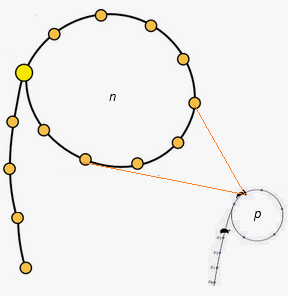
\includegraphics{proyeccion n en p.png}
    \caption{Lo que pasa en $n$ se proyecta en $p$}
    \par\small Fuente: Elaboración propia
\end{figure} \\
Por la naturaleza de $f$ hay un ciclo para $n$ y otro para $p$. Al ser $p$ un factor de $n$, es claro que $n>p$, por lo tanto el ciclo en $p$ será más pequeño, los valores que vayamos probando en $n$, a través de la función con ciclo, serán proyectados internamente en $p$. \\
Será como si la búsqueda se realizara operando directamente en módulo $p$, aún cuando no se conoce $p$ y sólo se trabaja módulo $n$. Al movernos en las secuencias $x_i$ y $y_j$ trabajamos con enteros distintos módulo $n$, sin embargo, por el juego de estructuras, dichos enteros colisionarán antes en $p$, serán congruentes módulo $p$ en algún momento de la secuencia, definitivamente. 

\subsection{Congruencia en $p$ y no congruencia en $n$}
Dado $n$ compuesto e impar, las secuencias $x_i, y_j$ generan ($x,y$) pares de números enteros módulo $n$ que en algún momento entran en un ciclo. \\
Ya se dijo que se espera que dichos números $x,y$ sean congruentes módulo $p$, el factor desconocido de $n$ (tal congruencia se revelaría, nítidamente, aplicándoles en la sombra el módulo $p$). \\
Ahora se añade otra condición, se esperamos además que $x,y$ sean enteros no congruentes módulo $n$. \\
Todo ello cuaja en el siguiente enunciado.

\begin{enunciado} [Extracción de un factor por colisión en Rho de Pollard]\label{enun:extraeFactor}\leavevmode\par 
Sea $n=p \cdot c$, donde $p$ es un factor primo de $n$ y por tanto $p \mid n$. \\ 
Si $x,y$ son tales que \\ 
$x \equiv y \pmod p$ \\ 
$x \not\equiv y \pmod n $ \\ 
Entonces $d = mcd(|x - y|,n)$ satisface $1 < d < n$ y es un factor no trivial de $n$ (múltiplo de $p$ o $p$ mismo)
\end{enunciado}

\begin{proof} Sea $d = mcd(|x - y|,n)$. \\
Si $x \equiv y \pmod p$, entonces por el Enunciado~\ref{enun:congrViaDivisib}, $p \mid (x - y)$. Por lo tanto, $(x-y)=kp$, luego $|x-y|=|kp|=p|k|$, por lo tanto: $p \mid |x-y|$. \\
Como $p \mid n$ entonces $p$ divide a ambos números $|x - y|$ y $n$, es decir, $p \mid |x-y|$ y $p \mid n$. \\
Por el Enunciado~\ref{enun:maspropMcd}.ix: $p \mid mcd(|x - y|,n)$, es decir, $p \mid d$. Luego, por el Enunciado~\ref{enun:propDivisibilidad}.ii: $d \geq p$. \\
Como $p$ es primo, $p > 1$, por lo tanto: $d > 1$. \\
Si $x \nequiv y \pmod n $, entonces $n \nmid (x - y)$. \\
Razonando por contradicción, supongamos que $d = n$. \\
Por lo tanto: $n = mcd(|x - y|,n)$. Y, por supuesto: $n \mid |x - y|$. \\
Luego, $n \mid (x - y)$, lo que contradice $n \nmid (x - y)$. \\
Ello invalida el supuesto y prueba que $d \neq n$. \\
Como $d = mcd(|x - y|,\, n)$, por definición $d \mid n$, luego  por el Enunciado~\ref{enun:propDivisibilidad}.ii: $d \leq n$. \\ 
Como $d \neq n$ y $d \leq n$ entonces: $d < n$. \\
Hemos probado que $1 < d < n$. \\
Como $d \mid n$, por definición, $d$ es un divisor propio no trivial de $n$. \\
Como $p \mid d$, entonces $d=pk'$, es decir, $d= mcd(|x - y|,n)$ es un múltiplo de $p$ (el cual puede ser $p$ mismo, o bien un múltiplo mayor).
\end{proof}

El objetivo no es mostrar que $x \equiv y \pmod p$ , sino aprovechar esa congruencia, cuando ocurre, para obtener un factor no trivial de $n$. No se sabe en qué paso ocurre tal congruencia, eso vive en un mundo al que no se tiene acceso directo, pero se puede razonar sobre él. \\
Lo que sí podemos hacer es calcular, en cada paso, $mcd(|x_i - y_j|, n)$, sin conocer $p$. Si en algún momento ocurre una colisión útil módulo un factor primo $p$ de $n$, antes de que ocurra la congruencia módulo $n$, el enunciado garantiza que el $mcd$ hará visible esa colisión como un factor no trivial de $n$, esa es la causa matemática de que $p$ aflore en el $mcd$. \\
El enunciado es la garantía de que ese cálculo, ciego a p, capturará el evento oculto en el momento en que ocurra, sin él no habría ninguna razón para creer que computar $mcd$'s sucesivos eventualmente revela $p$. \\
Pollard aprovecha una colisión parcial invisible para convertirla, mediante el $mcd$, en un factor visible de $n$, el factor $d$ es $p$ mismo o un múltiplo mayor, no importa, el enunciado garantiza que se obtiene dicho factor. \\
Como $p$ es un factor primo arbitrario de $p$, el razonamiento vale para cualquiera de los factores primos que pueda producir la colisión. \\
Sin esa congruencia parcial, el $mcd$ daría 1 y no serviría.  Sin la no congruencia módulo $n$ tampoco serviría, es el caso cuando el $mcd$ devuelve $n$. Los siguientes enunciados sustentan ello.

\begin{enunciado}
\label{enun:Rhomcd1}\leavevmode\par 
Sea $n=p \cdot c$, donde $p$ es un factor primo de $n$ y por tanto $p \mid n$. \\
Si $mcd(x - y, n) = 1$ entonces $x \nequiv y \pmod{p}$
\end{enunciado}

\begin{proof} Por contradicción. \\
Supongamos que $x \equiv y \pmod{p}$, por el Enunciado~\ref{enun:congrViaDivisib} $p \mid (x - y)$. \\
Es decir, $p \mid n$, también $p \mid (x - y)$. Por el Enunciado~\ref{enun:maspropMcd}.ix: $p \mid mcd(x - y, n)$. \\
Pero $mcd(x - y, n) = 1$. Por lo tanto: $p \mid 1$. \\
Lo que contradice que $p$ sea primo y prueba el enunciado.
\end{proof}

\begin{enunciado}
\label{enun:Rhomcd2}\leavevmode\par 
Sea $n=p \cdot c$, donde $p$ es un factor primo de $n$ y por tanto $p \mid n$. \\
Si $mcd(x - y, n) = n$ entonces $x \equiv y \pmod n$
\end{enunciado}

\begin{proof} Si $mcd(x - y, n) = n$ entonces $n \mid (x-y)$. \\
Luego, por el Enunciado~\ref{enun:congrViaDivisib}: $x \equiv y \pmod n$.
\end{proof}

\subsection{Velocidad de la colisión}
El Enunciado~\ref{enun:extraeFactor} muestra que buscar colisiones módulo $p$ funciona. \\ 
Resta engranar con una estrategia que indique cómo producir tales $x,y$ congruentes de forma eficiente. 
Es vital que sean congruentes módulo $p$, pero lo esencial es cómo generar esos pares de forma sistemática y rápida sin saber nada de $p$ (ahí es donde interviene el epimorfismo, sin él no queda claro por qué iterar módulo $n$ tendría algo que ver con el factor $p$). \\

Sería un error generar dos números $x,y$ completamente al azar en cada paso, calcular $mcd(x-y,n)$ y esperar que salga un valor $d$ tal que $1<d<n$: es un proceso muy lento (peor que buscar divisores uno por uno) y muy improbable (que dos números elegidos al azar difieran exactamente en un múltiplo de un factor de $n$, $x \equiv y \pmod p$, es de una probabilidad $1/p$ muy baja). \\
Pensemos en esta otra hipotética forma de hallar la colisión módulo $p$: guardar todos los valores, al generar uno nuevo compararlo con los anteriores (verificando si son congruentes módulo $p$), esto requiere poner en la lista cada número que va apareciendo para revisar si es congruente con uno que ya salió antes, la computadora se quedaría sin memoria al trabajar con números gigantescos. \\

La ventaja de usar $x_i$ y su subsecuencia $y_j$ (idea desprendida del algoritmo de Floyd para ver si una lista tiene ciclos) es que usa una sola secuencia, la confronta consigo misma y detecta una colisión prácticamente sin usar memoria: si la secuencia entra en un ciclo, $y_j$ (que es $x_{2i}$ que suele denominarse el corredor rápido o liebre) inevitablemente alcanzará a $x_i$ (que suele denominarse el corredor lento o tortuga) dentro del ciclo. No hay necesidad de almacenar toda la secuencia, sólo se requiere recordar dos variables en la memoria en todo momento: la posición actual del lento $x$ y la posición actual del rápido $y$. \\

La función $f$ módulo $n$ sirve para forzar los dos ciclos módulo $n$ y módulo $p$ (que no se ve, pero está ahí). \\
Tarde o temprano encontraremos $x_i \equiv y_j \pmod p $ antes de que $x_i \equiv y_j \pmod n $. \\
El principio del palomar (pigeonhole) dice: si se distibuye más elementos (números, palomas, etc.) que contenedores disponibles, al menos uno de los contenedores contendrá obligatoriamente varios elementos (que colisionan o chocan o se agrupan). \\
Como sólo hay un número finito de valores $p$ (contenedores), por el principio del palomar, al ir generando parejas diferentes (elementos) módulo $n$ ($p+1$ elementos, o más), tarde o temprano obligatoriamente habrá una colisión en el mundo secreto del módulo $p$: necesariamente hay dos índices $i \neq j$ (con $i,j \leq p$) tales que $x_i,y_j$ serán congruentes módulo $p$. \\
Y por la naturaleza del ciclo y su longitud, cada que generemos pares separados por (un múltiplo de) dicha longitud, seguirán existiendo colisiones. \\
Ello es una consecuencia puramente estructural de que el dominio $\Z/p\Z$ es finito y $f$ es una función determinista sobre él. \\

Pero la forma de trabajo de $f$ aporta otro asunto esencial además del ciclo: un análisis probabilista de su comportamiento, la velocidad. \\
¿Cuánto tarda en aparecer esa colisión? \\
$f$ genera una secuencia determinista de apariencia pseudoaleatoria, esto es crucial para aplicar tal análisis probabilístico con ayuda de la paradoja del cumpleaños. \\

\textbf{La paradoja del cumpleaños} \\
Sea un año de 365 días. \\
Dado un grupo de $N$ personas, hallaremos la probabilidad de que al menos dos personas cumplan años el mismo día. \\
Lo haremos hallando la probabilidad de que todos tengan cumpleaños distintos. \\
Cada persona tiene un cumpleaños igualmente probable e independiente. \\
La primera persona puede cumplir años en cualquiera de los 365 días: probabilidad 1. \\
La segunda persona debe caer en un día distinto:  probabilidad $\frac{364}{365}$. \\
Etc. \\
Probabilidad de que todos los $N$ cumpleaños sean distintos (P): \\
P = $\frac{365}{365} \cdot \frac{364}{365} \cdot \frac{363}{365} \cdots \frac{365-N+1}{365} = \prod_{i=0}^{N-1}\frac{365-i}{365} = \prod_{i=0}^{N-1}(1-\frac{i}{365})$ \\
Con $N=23, P=0.461655742$. \\
La probabilidad de que al menos dos coincidan es el complemento: $1-P$. \\
Con $N=23, 1-P=0.538344257$. \\
Con solo 23 personas, la probabilidad de que dos compartan cumpleaños, leída como porcentaje, es mayor al 50\%. \\

Aplicamos la misma idea para el caso de la colisión módulo $p$, la probabilidad $P$ de que, dados $k$ números, todos sean distintos es: \\
$P = \prod_{i=0}^{k-1}(1-\frac{i}{p})$ \\
$\ln P = \ln \prod_{i=0}^{k-1}(1-\frac{i}{p}) \qquad \;$ // aplicando logaritmo \\
$= \sum_{i=0}^{k-1}\ln\left(1-\frac{i}{p}\right) \qquad\qquad$  // propiedad de logaritmo \\
$\approx -\sum_{i=0}^{k-1}\frac{i}{p} \qquad\qquad\qquad \,\;$  // con $p$ grande $(i/p)\rightarrow 0$ y $\ln(1-x) \approx -x$ \\
$=- \frac{1}{p} \sum_{i=0}^{k-1}i$ \\
$ = -\frac{k(k-1)}{2p}$ \\
$\approx -\frac{k^2}{2p}$ \\
Es decir, $\ln P \approx -\frac{k^2}{2p}$. Luego, $P \approx e^{-k^2/(2p)}$. \\
La probabilidad de que al menos dos enteros colisionen es el complemento: \\
$1 - P \approx 1 - e^{-k^2/(2p)}$. \\
El valor de $k$ donde $1-P$ empieza a ser, visto como porcentaje, mayor al $50\%$ o, lo que es lo mismo, el valor de $k$ donde $P$ empieza a ser mayor a $0.5$, es decir, donde colisionar pasa a ser más probable que no, es: \\
$e^{-k^2/(2p)} > \frac{1}{2} \qquad \quad \, \,$ // aplicando logaritmo \\
$\ln e^{-k^2/(2p)} > \ln \frac{1}{2} \qquad$ \\
${-k^2/(2p)} > \ln \frac{1}{2} \qquad$ // obvio \\
$-k^2 > (2p) \ln \frac{1}{2} \qquad \,$ // $\cdot(-1)$  \\
$k^2 < (2p) \ln \frac{1}{2} \qquad \, \, \, \;$ // aplicando raíz cuadrada \\
$k < \sqrt 2 \sqrt p \sqrt{\ln \frac{1}{2}}\qquad$ // $c=\sqrt 2 \sqrt{\ln \frac{1}{2}}$ \\
$k < c \sqrt p$ \\
Es decir, el número $k$ de iteraciones antes de una (probable) colisión (que revele un factor de $n$) es del orden $O(\sqrt{p})$ y proviene de la misma lógica de la paradoja del cumpleaños. \\
Si cambiamos la meta de que $P>0.5$ por, digamos, $P>0.9$ y repetimos el cálculo, la constante cambiará pero el orden seguirá siendo $O(\sqrt{p})$. \\
Hemos simplificado la presentación, en vez de un umbral lo que corresponde es calcular el valor esperado del número de iteraciones hasta la colisión, que se obtiene así ($X$ es una variable aleatoria que representa el número de iteraciones en el que efectivamente ocurre la colisión): \\
$E[X] \approx \int_0^\infty P(X>k)\,dk \approx \int_0^\infty e^{-k^2/(2p)}\,dk = \sqrt{\frac{\pi}{2}} \sqrt{p}$. \\
Sin embargo, la presentación que se hizo es más sencilla y cumple el propósito. \\

El Enunciado~\ref{enun:cotaRaizdeN} muestra que el entero compuesto $n$ tiene un divisor $p$ tal que $p \leq \sqrt{n}$. \\
Por lo tanto: $\sqrt{p} \leq \sqrt (\sqrt{n})=n^{\frac{1}{4}}$. \\
Por ello la complejidad temporal promedio para encontrar un factor primo de $n$ se dice que es del orden O($n^{1/4}$) con este algoritmo.

\section{Fundamentos de las cribas}
En el contexto de la teoría de números, las cribas constituyen una familia de algoritmos deterministas diseñados para identificar números primos dentro de un conjunto finito de enteros mediante un proceso de filtrado sistemático. A diferencia de las pruebas de primalidad individuales, que verifican propiedades específicas de un solo número, una criba opera por eliminación: partiendo de una lista de candidatos, descarta iterativamente aquellos que son múltiplos de primos menores, dejando únicamente los números primos como resultado. Esta metodología, cuyo exponente clásico es la Criba de Eratóstenes, se fundamenta en principios aritméticos de divisibilidad y constituye la herramienta estándar para la generación eficiente de listas de primos.\\
La clasificación y evolución de estos métodos abarcan desde las aproximaciones más antiguas hasta algoritmos modernos optimizados, como la Criba de Atkin o las cribas segmentadas, cada uno con distintas complejidades computacionales y requerimientos de memoria. Comprender los fundamentos de estas técnicas no solo implica asimilar el criterio lógico de selección y marcado de múltiplos, sino también distinguir entre los distintos enfoques algorítmicos.\\
Es más útil, en varios casos, acompañar la teoría al momento de describir cribas específicas, así lo haremos, salvo algunos resultados que siguen a continuación.

\begin{enunciado}[Techo (ceil) como parte entera (floor)]\label{enun:ceilequivalentefloor}\leavevmode\par
Sea $b \geq 1$. $\lfloor \frac{a-1+b}{b} \rfloor  = \lceil \frac{a}{b}\rceil$
\end{enunciado}

\begin{proof}
Por el algoritmo de la división, Enunciado~\ref{enun:algDivision}:\\
$a = qb+r$, donde $q$ es el cociente y $r$ es el residuo, con $0 \leq r<b$.\\
Caso $r=0$:\\
$\lceil \frac{a}{b} \rceil$\\
$= \lceil \frac{qb}{b} \rceil$   \; \; \; \;  \; \; \; \; \; \; \; \;  // pues $a = qb+r$ y $r=0$\\
$= \lceil q \rceil = q$ \; \; \; \;  \; \; \; \; \; \;  // obvio\\
$= (q+1)-1$ \; \; \;  \; \; \; \;  // obvio \\
$= (q+1)+ \lfloor \frac{-1}{b} \rfloor$ \; \; \; \; //  pues $b \geq 1$ y $\lfloor \frac{-1}{b} \rfloor= -1$ \\
$= q+1+ \lfloor \frac{r-1}{b} \rfloor$ \; \; \; \;  \; //  pues $r=0$ \\
$=  \lfloor q+1+ \frac{r-1}{b} \rfloor$ \; \; \; \; \; // pues $q+1$ es entero \\
$=  \lfloor \frac{qb+b+ r -1}{b} \rfloor$  \; \; \; \;  \; \; \; \;  // obvio \\
$=  \lfloor \frac{qb+r+b-1}{b} \rfloor$ \; \; \; \;  \; \; \; \;  // obvio \\
$=  \lfloor \frac{a+b -1}{ b} \rfloor$ \; \; \; \;  \; \; \; \; \; \;  // pues  $a = qb+r$ \\
$=  \lfloor \frac{a-1+b}{b} \rfloor$ \; \; \; \; \; \;  \; \; \; \;   // obvio \\
Caso $r>0$:\\
Como $0<r<b$, entonces $1 \leq r$ y, como $r-1<r$ y $r<b$ entonces $r-1<b$.\\
$\lceil \frac{a}{b} \rceil$\\
$= \lceil \frac{qb+r}{b} \rceil$ \; \; \;  \; \; \; \; \; \; \; \;  // pues $a = qb+r$\\
$= \lceil q+ \frac{r}{b} \rceil$   \; \; \; \; \; \; \; \; \; \; // obvio \\
$= q+ \lceil \frac{r}{b} \rceil$ \; \; \; \; \; \; \; // pues $q$ es entero \\
$= q+1$  \; \; \; \; \; \; \; \; \; // pues $r<b$ y $\lceil \frac{r}{b} \rceil = 1$ \\
$= q+1+0$ \; \; \; \; \; \; // obvio \\
$= q+1+ \lfloor \frac{r-1}{b} \rfloor$ \; \; \; // pues  $r-1<b$ y $\lfloor \frac{r-1}{b} \rfloor = 0$
$=  \lfloor q+1+ \frac{r-1}{b} \rfloor$ \; \; \; // pues $q+1$ es entero \\
$=  \lfloor \frac{qb+b+ r -1}{b} \rfloor$  \; \; \; \;  \;  // obvio \\
$=  \lfloor \frac{qb+r+b-1}{b} \rfloor$ \; \; \; \; \;  // obvio \\
$=  \lfloor \frac{a+b -1}{ b} \rfloor$ \; \; \; \;  \; \; \;  // pues  $a = qb+r$ \\
$=  \lfloor \frac{a-1+b}{b} \rfloor$ \; \; \; \; \; \; \;   // obvio
\end{proof}

\begin{enunciado}[$p ^{2}$ impar]\label{enun:p2impar}\leavevmode\par
Si $p$ es impar entonces $p^2$ es impar
\end{enunciado}

\begin{proof}
Como $p$ es impar, entonces $p = 2k+1$. \\
$p ^{2} = (2k+1)^{2} = 4k^{2}+4k+1 = 2(k^{2}+2k)+1$, que evidentemente es impar. 
\end{proof}

\begin{enunciado}[Suma de números pares/impares]\label{enun:parimpar}\leavevmode\par
La sumas de dos números pares o dos números impares es par. La suma de un número impar con uno par es impar.
\end{enunciado}

\begin{proof}
Para $a$ y $b$ pares: $a = 2k$, $b = 2q$. Luego, $a+b = 2k+2q = 2(k+q)$ que evidentemente es par. \\
Para $a$ y $b$ impares: $a = 2k+1$, $b = 2q+1$. Luego, $a+b = 2k+1+2q+1 = 2k+2q+2 = 2(k+q+1)$ que evidentemente es par. \\
Para $a$ par y $b$ impar: $a = 2k$, $b = 2q+1$. Luego, $a+b = 2k+2q+1 = 2(k+q)+1$ que evidentemente es impar.
\end{proof}

\subsection{Elementos para la criba cuadrática}
\label{subsec:Fundcuadratica}
En este caso la criba no pretende hallar números primos sino enteros con $B$-suavidad. 

\begin{definicion} [$B$-suavidad]\label{def:Bsuavidad}
La definición genérica dice que un entero es $B$-suave si todos sus factores primos son menores o iguales que el entero $B$. \\
Pero en la criba cuadrática un entero es $B$-suave si todos sus factores primos están en un conjunto base de primos llamado la base $B$. \\
Decir que un entero sea $B$-suave es equivalente a decir que el entero tenga $B$-suavidad.
\end{definicion}

\begin{enunciado}[Principio general]\label{enun:PpioGeneral}\leavevmode\par
Sea $n$ impar y compuesto. \\
Si existen enteros $x,y$ tales que $x^2 \equiv y^2 \pmod n \,$, $\, x \nequiv \pm  y \pmod n$ \\
entonces $d=mcd(x-y,n)$ es un factor no trivial de $n$, es decir, $1< d <n$
\end{enunciado}

\begin{proof} \, \\
Como $x^2\equiv y^2\pmod n$, por el Enunciado~\ref{enun:congrViaDivisib} $n \mid (x^2-y^2)$, es decir, $n \mid (x-y)(x+y)$. \\
Sea $d=mcd(x-y,n)$. \\
Queremos demostrar que $1<d<n$. \\
$d>1$: \\
Supongamos, por contradicción, que $d=1$. \\
Como $x^2 \equiv y^2\pmod n$, además $-y^2  \equiv -y^2\pmod n$, entonces por el Enunciado~\ref{enun:propCongru}.iii: \\
$x^2-y^2 \equiv y^2-y^2 \pmod n$, es decir: $x^2-y^2 \equiv 0 \pmod n$. \\
Como $x^2-y^2 = (x-y)(x+y)$, entonces: \\
$(x-y)(x+y) \equiv 0 \pmod n$. \\
Como $d=1$, entonces $mcd(x-y,n)=1$. \\
Por el Enunciado~\ref{enun:existInvModular} $x-y$ tiene inverso módulo $n$. \\
Es decir, existe $a$ tal que $a(x-y) \equiv 1 \pmod n$. \\
Como $(x-y)(x+y) \equiv 0 \pmod n$, además $a \equiv a \pmod n$, entonces por el Enunciado~\ref{enun:propCongru}.iv: \\
$a(x-y)(x+y) \equiv a \cdot 0 \pmod n$. \\
Es obvio que $a \cdot 0 = 0$. Como $a(x-y) \equiv 1 \pmod n$ entonces por el Enunciado~\ref{enun:propCongru}.viii: \\
$(x+y) \equiv 0 \pmod n$. \\
Es decir, $x\equiv-y\pmod n$, contradiciendo la hipótesis $x \nequiv \pm y \pmod n$. \\
Por tanto, $d>1$. \\
$d<n$: \\
Supongamos, por contradicción, que $d=n$. \\
Es decir, $mcd(x-y,n)=n$. \\
Entonces $n \mid (x-y)$, por el Enunciado~\ref{enun:congrViaDivisib} $x \equiv y \pmod n$, lo cual contradice $x \nequiv \pm y \pmod n$. \\
Así que $d<n$. \\
Por consiguiente, $1< mcd(x-y,n) < n$. \\
Es decir, $d$ es un factor no trivial de $n$.
\end{proof}

El principio general incluye como supuesto que $x \nequiv \pm  y \pmod n$ pues de lo contrario no se obtiene un factor no trivial.

\begin{enunciado}[Por qué la congruencia es estéril]\label{enun:congrEsteril}\leavevmode\par
a) Si $x \equiv y \pmod n$, entonces $\gcd(x-y, n) = n$. \\
b) Si $x \equiv -y \pmod n$, entonces $\gcd(x+y, n) = n$.
\end{enunciado}

\begin{proof} \, \\
a) Como $x \equiv y \pmod n$, por el Enunciado~\ref{enun:congrViaDivisib}, $n \mid (x-y)$. \\
Como $n \mid n$, entonces $mcd(x-y, n) = n$. \\
b) Como $x \equiv -y \pmod n$, por el Enunciado~\ref{enun:congrViaDivisib}, $n \mid (x-(-y))$, es decir, $n \mid (x+y)$. \\
Como $n \mid n$, entonces $mcd(x+y,n) = n$. \\
En ambos casos el factor $n$ es trivial.
\end{proof}

\begin{enunciado}[Por qué la congruencia es estéril, segunda parte]\label{enun:congrEsteril2}\leavevmode\par
a) Sea $n$ un entero impar y compuesto. 
\\ Sea $B=\{p_{1},p_{2},\dots ,p_{m}\}$ una base primos tales que $\forall p_{i} \in B \,\, p_{i} \nmid n$. \\
Sean $x,y$ enteros tales que $x^{2} \equiv y^{2}\pmod n$. \\
Supongamos que $y$ se construye como producto de potencias de primos de $\mathcal{B}$ (es decir, $y$ es $B$-suave). \\
Supongamos además que: \\
a) $x \equiv y \pmod n$ entonces $mcd(x+y,n)=1$. \\
b) $x \equiv -y \pmod n$ entonces $mcd(x-y,n)=1$.
\end{enunciado}

\begin{proof} \, \\
Como $n$ es impar, $mcd(2,n)=1$, por tanto por el Enunciado~\ref{enun:maspropMcd}.x $mcd(2y,n)=mcd(y,n)$. \\
Por hipótesis, todo primo que divide a $y$ pertenece a $B$, y ningún primo de $B$ divide a $n$. Por lo tanto, $mcd(y,n)=1$. \\
a) Como $x \equiv y\pmod n$ y como $y \equiv y \pmod n$, por el Enunciado~\ref{enun:propCongru}.iii: $x+y\equiv 2y\pmod n$. \\
Luego, por el Enunciado~\ref{enun:maspropMcd}.xi, $mcd(x+y,\, n)=mcd(2y,n)$. \\
En consecuencia $mcd(x+y,n)=1$. \\
b) Como $x \equiv -y \pmod n$, $-y \equiv -y \pmod n$, por el Enunciado~\ref{enun:propCongru}.iii: $x-y \equiv -2y\pmod n$. \\
Luego, por el Enunciado~\ref{enun:maspropMcd}.xi y por el Enunciado~\ref{enun:propMcd}.ii: \\
$mcd(x-y,n)=mcd(-2y,n)=mcd(2y,n)$. \\
En consecuencia $mcd(x-y,n)=1$. \\
En ambos casos, si $mcd(x-y,n)=n$ (o $mcd(x+y,n)=n$), calcular $mcd(x+y,n)$ (o $mcd(x-y,n)$) es redundante, pues necesariamente dará el factor trivial $1$.
\end{proof}

\begin{enunciado}[Por qué la congruencia es estéril, tercera parte]\label{enun:congrEsteril3}\leavevmode\par
Sea $n$ un entero impar y compuesto. \\
Sean $x, y$ tales que $x^2 \equiv y^2 \pmod n$. \\
Entonces: \\
1) $mcd(x-y, n) = 1 \quad\Longleftrightarrow\quad x \equiv -y \pmod n \;\text{ y }\; mcd(y,n)=1$ \\
2) $mcd(x+y, n) = 1 \quad\Longleftrightarrow\quad x \equiv y \pmod n \;\text{ y }\; mcd(y,n)=1$
\end{enunciado}

\begin{proof}
Como $x^2 \equiv y^2 \pmod n$, por el Enunciado~\ref{enun:congrViaDivisib}: $n \mid (x-y)(x+y) \qquad$ (*) \\
\textit{1}) \\
$\Rightarrow$) Supongamos $mcd(x-y,n) = 1$. \\
De (*) y por el Enunciado~\ref{enun:propMcd}.viii, lema de Euclides: $n \mid (x+y)$, es decir, $n \mid (x-(-y))$. \\
Luego, por el Enunciado~\ref{enun:congrViaDivisib}, $x \equiv -y \pmod n$. Además $-y \equiv -y \pmod n$. \\
Entonces, por el Enunciado~\ref{enun:propCongru}.iii: $x - y \equiv -2y \pmod n$. \\
Luego, por el Enunciado~\ref{enun:maspropMcd}.xi, $mcd(x-y,n)=mcd(-2y,n)$. \\
Y por el por el Enunciado~\ref{enun:propMcd}.ii: $mcd(x-y,n)=mcd(2y,n)$. \\
Como $n$ es impar, $mcd(2,n)=1$, por tanto por el Enunciado~\ref{enun:maspropMcd}.x $mcd(2y,n)=mcd(y,n)$. \\ 
Es decir: $mcd(x-y,n)=mcd(y,n)$. Como $mcd(x-y,n) = 1$, entonces: \\
$mcd(y,n) = 1$. \\
$\Leftarrow$) Supongamos ahora que $x \equiv -y \pmod n$ y $mcd(y, n) = 1$. \\
Como $-y \equiv -y \pmod n$, de ello y de $x \equiv -y$ se sigue, por el Enunciado~\ref{enun:propCongru}.iii, que: \\
$x - y \equiv -2y \pmod n$. \\
Luego, por el Enunciado~\ref{enun:maspropMcd}.xi, $mcd(x-y,n)=mcd(-2y,n)$. \\
Y por el por el Enunciado~\ref{enun:propMcd}.ii: $mcd(x-y,n)=mcd(2y,n)$. \\
Como $n$ es impar, $mcd(2,n)=1$, por tanto por el Enunciado~\ref{enun:maspropMcd}.x $mcd(2y,n)=mcd(y,n)$. \\ 
Es decir: $mcd(x-y,n)=mcd(y,n)$. Como $mcd(y,n) = 1$, entonces: \\
$mcd(x-y,n) = 1$. \\
\textit{2}) \\
El razonamiento es completamente análogo.
\end{proof}

\subsubsection{Raíces cuadráticas, criterio de Euler y símbolos de Legendre y Jacobi} 
\label{subsubsec:JacobiYmas}
La Definición~\ref{def:congrcuadraticaraizde1modn} introduce la congruencia cuadrática pura: $x^2 \equiv a \pmod m$. \\
Se tiene la siguiente definición asociada.

\begin{definicion}[Definición amplia de residuo cuadrático] \, \\
$a$ es un residuo cuadrático módulo $m$ si existe un entero $x$ tal que $x^2 \equiv a \pmod {m}$.
\end{definicion}

\begin{ejemplo}
$9$ es un residuo cuadrático módulo $21$, según la definición amplia, pues existe $x=3$ tal que $3^2 \equiv 9 \pmod {21}$.
\end{ejemplo}

Se tiene esta otra definición asociada que podemos denominar definición estricta pues exige que $mcd(a,m)=1$.

\begin{definicion}[Residuo cuadrático]\label{def:residuocuadr} \, \\
$a$ coprimo con $m$ es un residuo cuadrático módulo $m$ si la congruencia $x^2  \equiv a \pmod {m}$ tiene solución.
\end{definicion}

\begin{ejemplo}
$9$ no es un residuo cuadrático módulo $21$ estricto pues $mcd(9,21)=3$. \\
$5$ es un residuo cuadrático módulo $11$ pues existe $x=4$ tal que $4^2 \equiv 5 \pmod {11}$ y $mcd(5,11)=1$.
\end{ejemplo}

$a$ es un cuadrado módulo $m$ es, quizás, un mejor nombre, pero en la  historia siempre se ha dicho que $a$ es un residuo cuadrático módulo $m$, de modo que respetaremos ello. \\
 
La definición estricta es la definición usual pues con la exigencia de coprimalidad, como se muestra en el Anexo~\ref{anexo:iso}, $(\Z/m\Z)^{*}$ es un grupo multiplicativo. \\
Las características de un grupo multiplicativo son altamente deseables, por ejemplo, todos sus elementos tienen inverso. El conjunto de residuos cuadráticos módulo $m$ es un subgrupo de dicho grupo multiplicativo, como lo muestra el siguiente enunciado.

\begin{enunciado} El conjunto de los residuos cuadráticos módulo $m$ que son coprimos con $m$ forma un subgrupo del grupo multiplicativo $(\Z/m\Z)^{*}$
\end{enunciado}

\begin{proof} Un elemento $a \in (\Z/m\Z)^*$  es un residuo cuadrático si existe un $ x \in (\Z/m\Z )^*$  tal que: \\
$ x^{2}\equiv a \pmod m$ \\
Este conjunto  es un subgrupo de $ (\Z/m\Z )^*$ pues verifica sus propiedades fundamentales: \\
. Identidad: El $1$  siempre es un residuo cuadrático porque $1^2 \equiv 1 \pmod m$. \\
. Cierre bajo el producto: Si $a$  y $ b$  son residuos cuadráticos, existen $ x$  e $ y$  tales que $x^2 \equiv a$  y $y^2 \equiv b$ . Entonces: $a \cdot b\equiv x^{2}\cdot y^{2}\equiv (x\cdot y)^{2} \pmod m$ .\\
Como $ (x \cdot y)^2$  es un cuadrado perfecto, $ a \cdot b$  también es un residuo cuadrático. \\
. Inversos: Si $a$  es un residuo cuadrático ($x^2 \equiv a$ ), podemos multiplicar ambos lados por el inverso de $x^{2}$  (que es $(x^{-1})^2$): $a\cdot (x^{-1})^{2}\equiv x^{2}\cdot (x^{-1})^{2}\equiv 1 \pmod m$. \\ 
Por lo tanto, $a^{-1} \equiv (x^{-1})^2 \pmod m$ , por lo que el inverso de $a$  también es un residuo cuadrático y pertenece al subgrupo.
\end{proof}

El caso particular  $x^2  \equiv n \pmod {p}$ con $p$ primo y $n$ un entero impar y compuesto es relevante pues se utiliza en la factorización de $n$ con la criba cuadrática. \\

En vez de decir que existe un entero $x$ tal que $x^2  \equiv n \pmod {p}$ (suficiente para decir que $n$ es un residuo cuadrático módulo $p$), también es usual decir hallar las raíces de $x^2  \equiv n \pmod {p}$. \\
Con $p$ primo cada elemento distinto del 0 del conjunto de base tiene inverso multiplicativo, con ello -como se ve en el Anexo~\ref{anexo:iso}- $(\Z/m\Z)^{*}$ es un cuerpo. \\
Es decir, no existen divisores de cero: si $ab \equiv 0 \pmod{p}$, entonces necesariamente $a \equiv 0$ o $b \equiv 0$. \\

Resolver $x^2 \equiv 1 \pmod{p}$ es resolver $x^2 - 1 \equiv 0 \pmod{p}$, es decir, $(x-1)(x+1) \equiv 0 \pmod{p}$. \\
Sin divisores de cero, el producto solo puede ser cero si uno de los factores lo es: \\
$x-1 \equiv 0 \pmod{p}$, es decir, $x \equiv 1 \pmod{p}$ \\
$x+1 \equiv 0 \pmod{p}$, es decir, $x \equiv -1 \pmod{p}$ \\
Al ser $x^2 - 1$ un polinomio de grado 2 no puede tener más de 2 raíces distintas.

\begin{ejemplo}
$2310 \bmod 13 = 9$. \\
Luego, $2310$ es un residuo cuadrático módulo $13$ pues existe $x=3$ tal que $3^2  \equiv 2310 \pmod {13}$. \\
Como $10^2 \bmod 13 = 100 \bmod 13 = 9$, con igual validez puede decirse que $2310$ es un residuo cuadrático módulo $13$ pues existe $x=10$ tal que $10^2  \equiv 2310 \pmod {13}$. \\
Dicho de la otra forma: hallemos las raíces de $x^2  \equiv 2310 \pmod {13}$. La raíces son $x=3,10$, hay solución.
\end{ejemplo}

\begin{ejemplo} Sea $p=11$. \\
Trabajaremos con el conjunto $\{1, 2, \dots, p-1\} = \{1, 2, \dots, 10\}$. \\
Al elevar al cuadrado los números del 1 al 10 y calcular su resto módulo 11, obtenemos:
\begin{itemize}
    \item $1^2 \equiv 10^2 \equiv 1 \pmod{11}$
    \item $2^2 \equiv 9^2 \equiv 4 \pmod{11}$
    \item $3^2 \equiv 8^2 \equiv 9 \pmod{11}$
    \item $4^2 \equiv 7^2 \equiv 5 \pmod{11}$
    \item $5^2 \equiv 6^2 \equiv 3 \pmod{11}$
\end{itemize}
El conjunto de residuos cuadráticos módulo 11 es $\{1, 3, 4, 5, 9\}$. 
Exactamente la mitad (5 de 10) de los elementos de $\{1, 2, \dots, 10\}$ son residuos cuadráticos distintos. \\
Nótese que $x^2 \equiv (p-x)^2 \pmod{p}$, es decir, $x^2 \equiv (11-x)^2 \pmod{11}$. \\
Es decir, cada número $x$ y su complemento $11-x$ producen el mismo residuo cuadrático módulo 11.
\end{ejemplo}

\begin{enunciado} [Número de residuos cuadráticos con $p$ primo]\label{enun:numResiduos}\leavevmode\par
Para $p$ un primo impar, exactamente la mitad $\frac{p-1}{2}$ de los números en el conjunto $\{1, 2, \dots, p-1\}$ son residuos cuadráticos distintos.
\end{enunciado}

\begin{proof}
Los cuadrados módulo $p$ de los números en $\{1,2,\dots,p-1\}$ son: \\
$1^2, \dots, (p-1)^2 \pmod{p}.$ \\
Como $(p-x)^2 = p^2 -2xp + x^2$, además que $p^2 -2xp + x^2 \equiv x^2 \pmod p$: \\
$x^2 \equiv (p-x)^2 \pmod{p}$ \\
Es decir, cada número $x$ y su complemento $p-x$ producen el mismo residuo cuadrático módulo $p$. \\
Por ello, los números $1,2,\dots,p-1$ se pueden agrupar en $\frac{p-1}{2}$ pares: \\
$(1, p-1), (2, p-2), \dots, \left(\tfrac{p-1}{2}, \tfrac{p+1}{2}\right)$. \\
Cada par genera el mismo residuo cuadrático módulo $p$.  \\
Por lo tanto, de los $p-1$ residuos cuadráticos, sólo hay $\frac{p-1}{2}$ valores distintos. \\
Tampoco es posible que dos pares distintos den el mismo resultado. En efecto, sean $x,y$ elementos de distintos pares. Supongamos que $x^2 \equiv y^2 \pmod p$, es decir, $x^2 - y^2 \equiv 0 \pmod p$. \\
Por la distributividad del producto sobre la suma: $x^2 - y^2 = (x-y)(x+y) $. \\
Entonces: $(x-y)(x+y) \equiv 0 \pmod{p}$. \\
Como $\Z/p\Z$, es un cuerpo, en la la Sección~\ref{sec:polinomios} se muestra que no tiene divisores de cero. \\
Por lo tanto, si $(x-y)(x+y) \equiv 0 \pmod{p}$, entonces: \\
$(x-y) \equiv 0 \pmod{p}$, o $(x+y) \equiv 0 \pmod{p}$. \\
Es decir: \\
$x \equiv y \pmod{p}$, o \\
$x \equiv -y \pmod{p}$, de donde se tiene: $x \equiv p-y \pmod{p}$.\\
Lo que contradice que $x,y$ sean de distintos pares. \\
Luego, todos los $\frac{p-1}{2}$ resultados tienen que ser estrictamente diferentes entre sí. \\
\end{proof}

El \textbf{Criterio de Euler} es un resultado de la teoría de números que permite determinar si un número es un residuo cuadrático módulo un primo $p$ sin necesidad de encontrar explícitamente sus raíces.

\begin{enunciado}[Criterio de Euler]\label{enun:criterioEuler}\leavevmode\par
Sea $p$ un número primo impar y sea $n$ un entero tal que $mcd(n,p) = 1$ (es decir, $p \nmid n$). Entonces: \\
$n^{\frac{p-1}{2}} \equiv
\begin{cases}
\,\,\; 1 \pmod{p} & \text{si } n \text{ es un residuo cuadrático módulo } p \\
-1 \pmod{p} & \text{si } n \text{ no es un residuo cuadrático módulo } p
\end{cases}$
\end{enunciado}

\begin{proof}
Por el Enunciado~\ref{enun:teorFermat} (pequeño teorema de Fermat) $n^{p-1} \equiv 1 \pmod p$. \\
Como $n^{p-1} = \left(n^{\frac{p-1}{2}}\right)^2$ entonces $\left(n^{\frac{p-1}{2}}\right)^2 \equiv 1 \pmod{p}$. \\
Como $-1 \equiv -1 \pmod{p}$, por el por el Enunciado~\ref{enun:propCongru}.iii: $\left(n^{\frac{p-1}{2}}\right)^2 - 1 \equiv 0 \pmod{p}$. \\
Sea $b = n^{\frac{p-1}{2}}$, entonces: $b^2 - 1 \equiv 0 \pmod{p}$. \\
Como se muestra en la Sección~\ref{sec:polinomios} $p(x)=x^2 - 1$ se puede factorizar como $p(x) = (x-1)(x+1)$. \\
Entonces: $(b-1)(b+1) \equiv 0 \pmod{p}$. \\
Como $\Z/p\Z$, es un cuerpo, en la misma sección se muestra que no tiene divisores de cero. Por lo tanto: \\
Si $(b-1)(b+1) \equiv 0 \pmod{p}$, entonces: $b-1 \equiv 0 \pmod{p}$, o $b+1 \equiv 0 \pmod{p}$. \\
Es decir: \\
$b \equiv 1 \pmod{p}$, o \\
$b \equiv -1 \pmod{p}$. \\
Es decir: \\
$n^{\frac{p-1}{2}} \equiv 1 \pmod{p}$, o \\
$n^{\frac{p-1}{2}} \equiv -1 \pmod{p}$. \\
Supongamos que $n$ es un residuo cuadrático. \\
Es decir, existe $x$ tal que $x^2 \equiv n \pmod{p}$. \\
Entonces, por el Enunciado~\ref{enun:propCongru}.ix: $(x^2)^{\frac{p-1}{2}} \equiv n^{\frac{p-1}{2}}$. Es decir: \\
$n^{\frac{p-1}{2}} \equiv x^{p-1}$. \\
Por el Enunciado~\ref{enun:teorFermat} (pequeño teorema de Fermat): $x^{p-1} \equiv 1 \pmod{p}$. La aplicación del pequeño teorema de Fermat es correcta pues $p \nmid x$.
En efecto, suponer que $p \mid x$, implica que $p \mid x^2$, lo que implica que $p \mid n$, contradiciendo que $mcd(n,p)=1$. \\
Así, si $n$ es un residuo cuadrático módulo $p$, el resultado es $1$: $n^{\frac{p-1}{2}} \equiv 1 \pmod{p}$. \\
Supongamos que $n$ no es un residuo cuadrático. \\
Sea $g(x) = x^{\frac{p-1}{2}} - 1$. \\
Tomemos un $b \in \{1,2,\dots,p-1\}$ que sea residuo cuadrático. \\
Con un razonamiento idéntico al caso anterior: $b^{\frac{p-1}{2}} \equiv 1 \pmod{p}$. \\
Es decir, todo residuo cuadrático es raíz de $g(x)$. \\
Por el Enunciado~\ref{enun:numResiduos}, para $p$ primo impar hay exactamente $\frac{p-1}{2}$ residuos cuadráticos. \\
Por el Enunciado~\ref{enun:numRaices}, $g(x)$  tiene a lo sumo $\frac{p-1}{2}$ raíces distintas, \\
Por lo tanto las raíces de $g(x)$ son exactamente los residuos cuadráticos y ningún otro elemento de $\{1,2,\dots,p-1\}$ es raíz. \\
Como $n$ no es residuo cuadrático, entonces no es raíz de $g(x)$, es decir, $n^{\frac{p-1}{2}} \not\equiv 1 \pmod p$. \\
Como $n^{\frac{p-1}{2}} \equiv 1 \pmod{p}$ o $n^{\frac{p-1}{2}} \equiv -1 \pmod{p}$, la única alternativa restante es $n^{\frac{p-1}{2}} \equiv -1 \pmod p$. \\
Así, si $n$ no es un residuo cuadrático módulo $p$, el resultado es $-1$: $n^{\frac{p-1}{2}} \equiv -1 \pmod{p}$. 
\end{proof}

El criterio de Euler da un algoritmo eficiente, mediante exponenciación rápida, para decidir si $n$ es residuo cuadrático módulo $p$, sin necesidad de probar todos los cuadrados. \\
Aunque hay otro modo igual o más eficiente para determinar ello. Requiere algo de notación adicional y resultados teóricos esenciales. \\

Cuando $p \mid n$: $p \mid (n-0)$. Por el Enunciado~\ref{enun:congrViaDivisib}: $n \equiv 0 \pmod p$. De modo que por el Enunciado~\ref{enun:congrEquiv} (transitividad de la relación de congruencia): $x^2  \equiv n \pmod {p}$ se reduce a $x^2  \equiv 0 \pmod {p}$, cuya unica solución es la trivial $x  \equiv 0 \pmod {p}$. \\
Es un caso degenerado. \\
Cuando $p \mid n$, entonces $mcd(p,n)>1$, por lo tanto $n$ no tiene inverso (no es unidad) módulo $p$, por lo que \underline{está fuera del dominio} en el que tiene sentido clasificar a $n$ como que sea o no sea residuo cuadrático; ni siquiera decir “caso degenerado” es propio: simplemente no aplica la noción de residuo cuadrático porque la definición está reservada al grupo multiplicativo $(\Z/n\Z)^{*}$.

El \textbf{símbolo de Legendre} $\legs{a}{p}$ es una función que permite identificar el carácter cuadrático de un número, para $p$ un primo impar se define como: \\
$\legs{n}{p} =
\begin{cases}
\,\,\; 1 & \text{si } n \text{ es un residuo cuadrático} \bmod p \\
-1 & \text{si } n \text{ no es un residuo cuadrático} \bmod p \\
\,\,\; 0 & \text{si } p \mid n \text{ (} $n$ \text{ fuera del dominio)}
\end{cases}$ 

\begin{ejemplo} \, \\
Sea $p=11$. \\
$\legs{3}{11} = 1$, pues $3$ es un  residuo cuadrático módulo $11$ (existe $x=5$ tal que $5^2 \equiv 3 \pmod{11}$). \\
$\legs{6}{11} = -1$, pues $6$ no es un  residuo cuadrático módulo $11$ (no existe $x$ tal que $x^2 \equiv 6 \pmod{11}$). \\
$\legs{22}{11} = 0$, pues $11 \mid 22$, $22$ está fuera del dominio. \\
\end{ejemplo}

Se puede calcular el símbolo de Legendre con un cálculo previo del $mcd(n,p)$ y en caso de ser $1$, vía el criterior de Euler. \\
De hecho es aceptable y usual una definición alterna con tal criterio: \\
$\legs{n}{p} \equiv n^{\frac{p-1}{2}} \pmod p$ \\
Con el plus de que si $\legs{n}{p}=0$, entonces $n^{\frac{p-1}{2}} \equiv 0 \pmod p$, que por el  Enunciado~\ref{enun:congrViaDivisib}, implica que $p \mid n^{\frac{p-1}{2}}$, y al ser $p$ primo, por el Enunciado~\ref{enun:propDivprim}.ii implica que $p \mid n$. \\

Otro modo de calcular el símbolo de Legendre es a través del cálculo del siguiente otro símbolo asociado. \\

El \textbf{símbolo de Jacobi} $\jac{n}{m}$, otra función, es una generalización matemática del símbolo de Legendre, para $m$ un entero positivo impar con factorización en primos (no necesariamente distintos) $m=p_1p_2\cdots p_k$ se define como el producto de símbolos de Legendre: \\
$\jac{n}{m} = \legs{n}{p_1} \legs{n}{p_2} \cdots \legs{n}{p_k}$. \\
Por convención, $\jac{n}{1}=1$ para todo $n$. \\

El símbolo de Jacobi tiene una alta relevancia computacional, de sus propiedades, que básicamente son una extensión de las propiedades del símbolo de Legendre al caso de $m$ impar y compuesto, se desprende un algoritmo que agiliza el cálculo de $\jac{n}{m}$. \\

Es obvio que cuando $m=p$, con $p$ primo, el símbolo de Jacobi se reduce exactamente al símbolo de Legendre. \\
En la práctica, no se distingue la notación, se entiende que si el denominador es primo, se trata del símbolo de Legendre, si es compuesto impar, se trata del símbolo de Jacobi, así el denominador determina cuál de los dos símbolos está en juego. \\
También, cuando $m=p$, con $p$ primo, la interpretación de los resultados es la de Legendre. \\
Tal interpretación, en el contexto de residuo cudrático o no, varía en cambio cuando $m$ es compuesto: \\
$\jac{n}{m} =
\begin{cases}
\,\,\; 1 & \text{ambiguo} \\ 
-1 & \text{si } n \text{ no es un residuo cuadrático} \bmod m \\
\,\,\; 0 & \text{si } mcd(n,m)>1 \text{ (} $n$ \text{ fuera del dominio)}
\end{cases}$ 

\begin{enunciado}\label{enun:nResidpiResid}\leavevmode\par
Sea $m$ un entero positivo impar con factorización en primos (no necesariamente distintos) $m=p_1p_2\cdots p_k$. \\
Si existe $x$ tal que $x^2 \equiv n \pmod m$ entonces para todo $p_i$ tal que $p_i \mid m$: $x^2 \equiv n \pmod {p_i}$.
\end{enunciado}

\begin{proof}
Existe $x$ tal que: $x^2 \equiv n \pmod m$. \\
Entonces, por el Enunciado~\ref{enun:congrViaDivisib}, $m \mid (x^2 - n)$, es decir, $(x^2 - n)=qm$. \\
Para todo $p_i$ tal que $p_i \mid m$ resulta que $m=kp_i$. Luego: \\
$(x^2 - n)=qkp_i$, es decir, $p_i \mid (x^2 - n)$, es decir: \\
Para todo $p_i$ tal que $p_i \mid m$: $x^2 \equiv n \pmod {p_i}$.
\end{proof}

\begin{enunciado} Si $\jac{n}{m} = -1$, entonces $n$ no es residuo cuadrático módulo $m$.
\end{enunciado}

\begin{proof}
Probaremos la contrarrecíproca: \\
Si $n$ es residuo cuadrático módulo $m$, entonces $\jac{n}{m} \neq -1$. \\
Sea $m = p_1 \cdots p_k$ (los primos -no necesariamente distintos- son impares pues $m$ es impar). \\
Por definición de residuo cuadrático: $mcd(n,m)=1$. \\
Por definición del símbolo de Jacobi: $\jac{n}{m} = \legs{n}{p_1} \legs{n}{p_2} \cdots \legs{n}{p_k}$. \\
Como $n$ es residuo cuadrático módulo $m$, entonces $mcd(n,m)=1$. \\
Por lo tanto, para todo $p_i$ tal que $p_i \mid m$: $mcd(n,p_i)=1$. En efecto, si suponemos que existe algún $p_i$ tal que $mcd(n,p_i) \neq 1$, entonces como $p_i$ es primo, necesariamente $mcd(n,p_i)=p_i$, lo que implica $p_i \mid n$, que junto a $p_i \mid m$ implican que $mcd(n,m) \geq p_i >1$, los que contradice $mcd(n,m)=1$. \\
Como $n$ es residuo cuadrático módulo $m$, entonces por el Enunciado~\ref{enun:nResidpiResid}, $n$ es residuo cuadrático módulo $p_i$. \\
Luego el símbolo de Legendre devuelve: $\legs{n}{p_i} = 1$. \\
Entonces $\jac{n}{m} = \legs{n}{p_1} \legs{n}{p_2} \cdots \legs{n}{p_k} = 1 \cdot \ldots \cdot 1 = 1 \neq -1$.
\end{proof}

\begin{ejemplo} \, \\
Es fácil determinar que el conjunto de residuos cuadráticos módulo: \\
. $3$ es $\{1\}$ \\
. $5$ es $\{1,4\}$ \\
Para $n = 15 = 3 \cdot 5$: \\
$x^2 \bmod 15 = 1 \,\;$ para $x=\{1,4,11,14\}$. \\
$x^2 \bmod 15 = 4 \,\;$ para $x=\{2,7,8,13\}$. \\
$x^2 \bmod 15 = 6 \,\;$ para $x=\{6,9\}$. \\
$x^2 \bmod 15 = 9 \,\;$ para $x=\{3,12\}$. \\
$x^2 \bmod 15 = 10$ para $x=\{5,10\}$. \\
$n=\{3,6,9,12\}$ caen fuera del dominio pues $mcd(n,15)=3>1$. \\
$n=\{5,10\}$ caen fuera del dominio pues $mcd(n,15)=5>1$. \\
Luego, el conjunto de residuos cuadráticos módulo 15 es $\{1, 4\}$. \\ 
$\jac{5}{15} = \legs{5}{3} \legs{5}{5} = (-1)(0) = 0$, $mcd(5,15)=5>1$, $5$ está fuera del dominio; nótese que $15 \nmid 5$. \\
$\jac{7}{15} = \legs{7}{3} \legs{7}{5} = (1)(-1) = -1$, entonces 7 no es residuo cuadrático módulo 15.\\
$\jac{2}{15} = \legs{2}{3} \legs{2}{5} = (-1)(-1) = 1$, pero $2$ no es residuo cuadrático módulo $15$. \\
$\jac{4}{15} = \legs{4}{3} \legs{4}{5} = \legs{1}{3} \legs{4}{5} = (1)(1) = 1$, en efecto $4$ es residuo cuadrático módulo $15$.
\end{ejemplo}

El ejemplo ilustra la ambigüedad del valor $1$.  \\

En general Jacobi no nos dice si $n$ es un residuo cuadrático como lo hace Legendre, su valor está en que propone un procedimiento algorítmico que acelera el cálculo. \\
En el caso de $m=p$ con $p$ primo, el resultado $1$ sí se interpreta como indicador de que $n$ es residuo cuadrático.

El algoritmo se basa en propiedades muy conocidas. 

\begin{enunciado}[Periodicidad en Legendre] \, \\
Si $a \equiv b \pmod {p}$, entonces $\legs{a}{p} = \legs{b}{p}$
\end{enunciado}

\begin{proof} \, \\
Como $a\equiv b \pmod p$, por el Enunciado~\ref{enun:congrViaDivisib}, $p \mid (a-b)$, es decir, $a=b+kp$. \\ 
Queremos demostrar que $\legs{a}{p} =\legs{b}{p}$. Para ello, analizamos los dos casos posibles según la divisibilidad por $p$. \\
Caso $p \mid a$, es decir, $a \equiv 0 \pmod p$. \\
Como $p \mid a$, por definición $\legs{a}{p}=0$. \\
Como $a \equiv b \pmod p$ y $a \equiv 0 \pmod p$, por la transitividad de la congruencia: $b\equiv 0 \pmod p$. \\
Por el Enunciado~\ref{enun:congrViaDivisib}, $p \mid b$ y por definición $\legs{b}{p}=0$. \\
Así, en este caso, $\legs{a}{p} =\legs{b}{p} = 0$. \\
Caso $p \nmid a$, es decir, $a \nequiv 0 \pmod p$. \\
Como $p \nmid a$, entonces $p \nmid b$. En efecto, suponer que $p \mid b$ implica que $p \mid b + kp$, es decir, $p \mid a$, contradiciendo que $p \nmid a$. \\
De modo que, por definición, el símbolo de Legendre solo puede tomar los valores $1$ o $-1$. \\
Subcaso $\legs{b}{p} = 1$. \\
Por definición, esto significa que $b$ es un residuo cuadrático módulo $p$. Es decir, existe un entero $x$ tal que: $x^{2}\equiv b \pmod p$. \\
Como $a \equiv b \pmod p$, por la transitividad de la congruencia, resulta: $x^{2}\equiv a \pmod p$. \\
Es decir, $a$ también es un residuo cuadrático módulo $p$, por lo que $\legs{a}{p} = 1$. \\
Subcaso $\legs{b}{p} = -1$. \\
Por definición, esto significa que $b$ no es un residuo cuadrático módulo $p$, es decir, la ecuación $x^2 \equiv b \pmod p$ no tiene solución en los enteros. \\
Si suponemos que $\legs{a}{p} = 1$, ello implica que existe un entero $y$ tal que: $y^2 \equiv a \pmod p$. \\
Como $a \equiv b \pmod p$, por la transitividad de la congruencia, resulta: $y^2 \equiv b \pmod p$. \\
Ello contradice el hecho de que $b$ no es un residuo cuadrático módulo $p$. \\
Ello invalida el supuesto y necesariamente $\legs{a}{p} = -1$.
\end{proof}

\begin{enunciado}[Periodicidad en Jacobi] \, \\
Sea $m$ un entero positivo impar con factorización en primos (no necesariamente distintos) $m=p_1p_2\cdots p_k$. \\
Si $a \equiv b \pmod {m}$, entonces $\jac{a}{m} = \jac{b}{m}$
\end{enunciado}

\begin{proof} \, \\
Por definición: $\jac{a}{m} = \legs{a}{p_1} \legs{a}{p_2} \cdots \legs{a}{p_k}$. \\
Por un razonamiento análogo al del Enunciado~\ref{enun:nResidpiResid}: si  $a \equiv b \pmod {m}$ entonces para todo $p_i$ tal que $p_i \mid m$: $a \equiv b \pmod {p_i}$. \\
Como $a \equiv b \pmod {p_i}$, por la periodicidad en Legendre para cada $p_i$ : $\legs{a}{p_i} = \legs{b}{p_i}$. Es decir: \\
$\jac{a}{m} = \legs{b}{p_1} \legs{b}{p_2} \cdots \legs{b}{p_k}$. \\
Tomando el producto: \\
$\jac{a}{m}= \legs{b}{p_1} \legs{b}{p_2} \cdots \legs{b}{p_k} =\jac{b}{m}$. 
\end{proof}

\begin{enunciado}[Multiplicatividad en Legendre] \, \\
$\legs{ab}{p} = \legs{a}{p} \legs{b}{p}$
\end{enunciado}

\begin{proof} \, \\
Como $(ab)^{\frac{p-1}{2}} \equiv a^{\frac{p-1}{2}} \cdot b^{\frac{p-1}{2}} \pmod{p}$. \hfill (*) \\
$\legs{ab}{p} \equiv (ab)^{\frac{p-1}{2}} \qquad \qquad \qquad \qquad \qquad \;$ por la definición alterna usando el criterio de Euler \\
${}\qquad \; \equiv a^{\frac{p-1}{2}} \cdot b^{\frac{p-1}{2}} \pmod{p} \qquad \qquad \quad$ por (*) \\
Por la definición alterna: $\legs{a}{p} \equiv a^{\frac{p-1}{2}} \pmod p$ y $\legs{b}{p} \equiv b^{\frac{p-1}{2}} \pmod p$. Por el Enunciado~\ref{enun:propCongru}.iv: \\
$\legs{a}{p} \legs{b}{p} \equiv a^{\frac{p-1}{2}} b^{\frac{p-1}{2}} \pmod p$ \\
Por la transitividad de la congruencia: \\
$\legs{ab}{p} \equiv \legs{a}{p} \legs{b}{p}$
\end{proof}

\begin{enunciado}[Multiplicatividad en Jacobi] \, \\
Sea $m$ un entero positivo impar con factorización en primos (no necesariamente distintos) $m=p_1p_2\cdots p_k$. \\
$\legs{ab}{m} = \legs{a}{m} \legs{b}{m}$
\end{enunciado}

\begin{proof} \, \\
$\legs{ab}{m} = \legs{ab}{p_1} \legs{ab}{p_2} \cdots \legs{ab}{p_k} \qquad \qquad \qquad \quad \;$ por definición \\
$= \legs{a}{p_1}\legs{b}{p_1} \legs{a}{p_2}\legs{b}{p_2} \cdots \legs{a}{p_k}\legs{a}{p_k} \qquad \quad \,$ por la multiplicatividad de Legendre \\
$= \legs{a}{p_1}\legs{a}{p_2} \cdots \legs{a}{p_k} \legs{b}{p_1}\legs{b}{p_2} \cdots \legs{b}{p_k} \qquad$ reorganizando \\
$= \legs{a}{m} \legs{b}{m} \qquad\qquad\qquad\qquad\qquad\qquad\qquad \; \,$ por definición
\end{proof}

\begin{enunciado}\label{enun:parImpar1raley}\leavevmode\par
a) $\frac{p-1}{2}$ es par si y sólo si $p \equiv 1 \pmod 4$ \\
b) $\frac{p-1}{2}$ es impar si y sólo si $p \equiv 3 \pmod 4$
\end{enunciado}

\begin{proof} \, \\
a) $\Rightarrow$  \\
$\frac{p-1}{2} = 2k$ pues es un número par, por lo tanto $p-1 = 4k$, es decir: $4 \mid p-1$. Por el Enunciado~\ref{enun:congrViaDivisib}: \\
$p\equiv 1 \pmod 4$. \\
a) $\Leftarrow$ \\
Como $p \equiv 1 \pmod 4$, por el Enunciado~\ref{enun:congrViaDivisib}, $4 \mid (p - 1)$, por lo tanto $p-1 = 4k = 2 \cdot 2k$, de donde se deduce que $\frac{p-1}{2} = 2k$, es decir: \\
$\frac{p-1}{2}$ es un número par. \\
b) $\Rightarrow$  \\
$\frac{p-1}{2} = 2k+1$ pues es un número impar, por lo tanto $p-1 = 4k+2$, luego $p-3 = 4k$, es decir: $4 \mid p-3$. Por el Enunciado~\ref{enun:congrViaDivisib}: \\
$p\equiv 3 \pmod 4$. \\
b) $\Leftarrow$ \\
Como $p \equiv 3 \pmod 4$, por el Enunciado~\ref{enun:congrViaDivisib}, $4 \mid (p - 3)$, por lo tanto $p-3 = 4k$, es decir, $p-1 = 4k+2 = 2(2k+1)$, de donde se deduce que $\frac{p-1}{2} = 2k+1$, es decir: \\
$\frac{p-1}{2}$ es un número impar. 
\end{proof}

\begin{enunciado}[1ra ley suplementaria en Legendre] \, \\
$\legs{-1}{p} = 
\begin{cases}
1 & \text{si } p \equiv 1 \pmod 4, \\
-1 & \text{si } p \equiv 3 \pmod 4.
\end{cases}$
\end{enunciado}

\begin{proof} Por la definición alterna usando el criterio de Euler: \\
$\legs{-1}{p} = (-1)^{\frac{p-1}{2}}$. \\
Es evidente que: \\
Si $\frac{p-1}{2}$ es par, entonces $(-1)^{\frac{p-1}{2}} = 1$. \\
Si $\frac{p-1}{2}$ es impar, entonces $(-1)^{\frac{p-1}{2}} = -1$. \\
Por el Enunciado~\ref{enun:parImpar1raley}: \\
$\frac{p-1}{2}$ es par si y sólo si $p \equiv 1 \pmod{4}$. \\
$\frac{p-1}{2}$ es impar si y sólo si $p \equiv 3 \pmod{4}$. \\
Lo que prueba el enunciado.
\end{proof}

\begin{enunciado}[1ra ley suplementaria en Jacobi] \, \\
Sea $m$ un entero positivo impar con factorización en primos (no necesariamente distintos) $m=p_1p_2\cdots p_k$. \\
$\jac{-1}{m} = (-1)^{\frac{m-1}{2}}$
\end{enunciado}

\begin{proof} \, \\
$\jac{-1}{m} = \legs{-1}{p_1} \cdots \legs{-1}{p_k} \qquad$ por definición \\
$ = (-1)^{\frac{p_1 - 1}{2}} \cdot \ldots \cdot (-1)^{\frac{p_k - 1}{2}} \quad$ por la 1ra ley suplementaria en Legendre \\
$ = (-1)^{\sum_{i=1}^k \frac{p_i - 1}{2}} \qquad \qquad \quad \; \,\,$ agrupando exponentes \\
$ = (-1)^{\frac{m-1}{2}} \qquad \qquad \qquad \quad \;$ pues $\sum_{i=1}^k \frac{p_i - 1}{2} \equiv \frac{m-1}{2} \pmod{2}$ \\
En efecto la paridad de $\sum_{i=1}^k \frac{p_i - 1}{2}$ es la misma que la de $\frac{m-1}{2}$, es decir: \\
$\sum_{i=1}^k \frac{p_i - 1}{2} \equiv \frac{m-1}{2} \pmod{2}$. \\
Por inducción sobre $k$: \\
Caso base ($k=1$): Es decir, $m=p_1$. \\
El lado izquierdo es: $\frac{p_1 - 1}{2}$. \\
El lado derecho es: $\frac{p_1-1}{2}$. \\
Son iguales. \\
Hipótesis Inductiva: El enunciado es cierto para k.\\
Paso inductivo ($k+1$): Sea $m=p_1p_2\cdots p_k$. \\
Sea $M=m\cdot p_{k+1}=p_1p_2\cdots p_kp_{k+1}$. \\
Como $m$ y $p_{k+1}$ son impares, $M$ también es impar. \\
Consideremos la siguiente expresión: $\frac{M-1}{2}-\left(\frac{m-1}{2}+\frac{p_{k+1}-1}{2}\right)$. \\
Sustituyendo $M=mp_{k+1}$: \\
$\frac{M-1}{2}-\left(\frac{m-1}{2}+\frac{p_{k+1}-1}{2}\right)$ \\
$=\frac{mp_{k+1}-1-(m-1)-(p_{k+1}-1)}{2}$ \\
$=\frac{mp_{k+1}-m-p_{k+1}+1}{2}$ \\
$=\frac{(m-1)(p_{k+1}-1)}{2}$ \\
Como $m$ y $p_{k+1}$ son impares, $m-1$ y $p_{k+1}-1$ son pares, los podemos escribir así: \\
$m-1=2a$, $p_{k+1}-1=2b$. Entonces: \\ 
$\frac{(m-1)(p_{k+1}-1)}{2} =\frac{(2a)(2b)}{2}=2ab$. \\
Luego: \\
$\frac{M-1}{2}-\left(\frac{m-1}{2}+\frac{p_{k+1}-1}{2}\right)=2ab\equiv 0\pmod 2$. \\
Por lo tanto, $\frac{M-1}{2}-\frac{p_{k+1}-1}{2} \equiv \frac{m-1}{2} \pmod 2$\\
Por hipótesis inductiva: $\frac{m-1}{2}\equiv \sum_{i=1}^k \frac{p_i-1}{2}\pmod 2$.
Por la transitividad de la congruencia: \\
$\frac{M-1}{2}-\frac{p_{k+1}-1}{2} \equiv \sum_{i=1}^k \frac{p_i-1}{2}\pmod 2$. \\
Por lo tanto: \\
$\frac{M-1}{2} \equiv \sum_{i=1}^k \frac{p_i-1}{2}+\frac{p_{k+1}-1}{2} =\sum_{i=1}^{k+1}\frac{p_i-1}{2}\pmod 2$. \\
Lo que prueba el caso $k+1$. \\
Los tres casos prueban la afirmación.
\end{proof}

\begin{enunciado}[Lema de Gauss]\label{enun:lemaGauss}\leavevmode\par
Sea $p$ un primo impar. \\
Sea $a$ un entero tal que $mcd(a,p)=1$. \\
Sea $S$ el conjunto formado por los residuos canónicos módulo $p$ de los números $a, 2a, 3a, \dots, \frac{p-1}{2}a$. \\
Si $k$ representa el número de tales residuos que son mayores que $\frac{p}{2}$, entonces $\legs{a}{p} = (-1)^{k}$
\end{enunciado}

\begin{proof} \, \\
Sea $t = \frac{p-1}{2} - k$, es decir, $k+t = \frac{p-1}{2}$. \\
Para cada entero $m$ tal que $1 \leq m \leq \frac{p-1}{2}$, sea $r_m$ el residuo canónico de $ma$ módulo $p$. Esto significa que cada $r_m$ es el único entero que cumple estrictamente la cláusula de acotación: $r_m \equiv ma \pmod p \quad \text{con} \quad 0 < r_m < p$. \\ 
Se excluye el $0$ pues $mcd(a,p)=1$. \\
Representaremos al conjunto de estos residuos como $S = \{r_1, r_2, \dots, r_{\frac{p-1}{2}}\}$ dividiéndolo en dos subgrupos: \
$S = \{ a_{1}, a_{2}, \dots, a_{t}, b_{1}, b_{2}, \dots, b_{k} \}$, donde $\forall i \; a_{i} < \frac{p}{2}$ con $i \in [1,t]$, $\forall j \; b_{j} > \frac{p}{2}$ con $j \in [1,k]$. \\
 Es decir: $\{ a_{1},\ldots,a_{t},b_{1},b_{2},\ldots,b_{k} \} = \{ r_1,\ldots,r_{\frac{p-1}{2}} \}$. \\
Nótese que por la acotación de los $r_m$, se cumple estrictamente que $0 < a_i < \frac{p}{2}$ y $\frac{p}{2} < b_j < p$. Además, como $p$ es impar, $\frac{p}{2}$ no es un entero. \\
(1) Todos los elementos de $S$ son incongruentes módulo $p$ y diferentes entre sí. En efecto: \\
Suponer que $m_{1}a \equiv m_{2}a \pmod{p}$ con $m_{1} \ne m_{2}$, implica, por el Enunciado~\ref{enun:congrViaDivisib}, que $p \mid (m_{1}-m_{2})a$. Como $mcd(a,p)=1$, entonces por el lema de Euclides -Enunciado~\ref{enun:propMcd}.viii- $p \mid (m_{1}-m_{2})$, lo que contradice que $p \nmid (m_{1}-m_{2})$, cosa cierta por el Enunciado~\ref{enun:propDivisibilidad}.iv y el hecho de $(m_{1}-m_{2}) < p$. Contradicción que prueba la afirmación. \\
¿Cuál es el valor más grande (cota superior) que puede tomar $(m_{1}-m_{2})$? Se lo obtiene tomando el valor máximo para $m_{1}$, que es $\frac{p-1}{2}$, y el valor mínimo que puede tomar $m_{2}$, que es $1$, por tanto la cota superior es $\frac{p-1}{2} - 1 < \frac{p-1}{2} < p$. Es decir, efectivamente $(m_{1}-m_{2}) < p$. \\
(2) $\forall i,j \; a_{i} \ne p-b_{j}$. En efecto: \\
Suponer que $a_{i} = p-b_{j}$ implica que $a_{i}+b_{j} \equiv 0 \pmod{p}$. Por la forma de construir el conjunto $S$, existen enteros únicos $m_i, m_j \in [1,\frac{p-1}{2}]$ con $m_{i} \ne m_{j}$ tales que $a_{i} \equiv m_{i}a \pmod p$, $b_{j} \equiv m_{j}a \pmod p$, entonces resulta que $m_{i}a + m_{j}a \equiv 0 \pmod{p}$. Luego, por el Enunciado~\ref{enun:congrViaDivisib}, $p \mid (m_{i}+m_{j})a$ y como $mcd(a,p)=1$, por el Enunciado~\ref{enun:propMcd}.viii, $p \mid (m_{i}+m_{j})$, lo que contradice que $p \nmid (m_{1}+m_{2})$, cosa cierta por el Enunciado~\ref{enun:propDivisibilidad}.iv y el hecho de $(m_{1}+m_{2}) < p$. Contradicción que prueba la afirmación. \\
¿Cuál es el valor más grande (cota superior) que puede tomar $(m_{1}+m_{2})$? Se lo obtiene tomando el valor máximo para $m_{1}$, que es $\frac{p-1}{2}$, y el valor máximo para $m_{2}$ que, como $m_{i} \ne m_{j}$, es $\frac{p-1}{2} - 1$, por tanto la cota superior es $\frac{p-1}{2} + \frac{p-1}{2} - 1 = p-2 < p$. Es decir, $(m_{1}+m_{2}) < p$. \\
Por la forma de representar S: \\
$\frac{p}{2} < b_{j} \qquad \quad \;$ // $\cdot (-1)$ \\
$- \frac{p}{2} > -b_{j} \qquad$ // $+ p$ \\
$p - \frac{p}{2} > p-b_{j}$ \\
Es decir: $p-b_{j} < \frac{p}{2}$ \\
Por ser $b_j$ un residuo canónico: \\
$b_j < p \qquad$ // $- b_j$ \\
$0 < p - b_j$ \\
Es decir: $\forall j \;\, 0 < p-b_{j} < \frac{p}{2}$. \\
Consideremos los $\frac{p-1}{2}$ números: $p-b_{1}, p-b_{2}, \dots, p-b_{k}, a_{1}, a_{2}, \dots, a_{t}$. \\
De (2) sabemos que $a_{i} \ne p-b_{j}$. \\
De (1) que todos los números en $S$ son diferentes, por tanto los $b_j$ son diferentes entre sí, como consecuencia todos los $p-b_j$ también son diferentes entre sí. \\
Recién probamos que $0 < p-b_{j} < \frac{p}{2}$ y, por la forma de representar $S$, se sabe que $a_{i} < \frac{p}{2}$. \\
Por lo tanto, los $\frac{p-1}{2}$ enteros $p-b_{1}, p-b_{2}, \dots, p-b_{k}, a_{1}, a_{2}, \dots, a_{t}$ son todos diferentes y menores que $\frac{p}{2}$. \\
Luego ellos son simplemente los números $1, 2, \dots, \frac{p-1}{2}$ en algún orden. \\
Por lo tanto: \\
$1 \cdot 2 \cdot \ldots \cdot \frac{p-1}{2} \equiv (p-b_{1})(p-b_{2})\cdots(p-b_{k})a_{1}a_{2}\cdots a_{t} \pmod{p}$ \\
Es decir: \\
$\left(\frac{p-1}{2}\right)! \equiv (p-b_{1})(p-b_{2})\cdots(p-b_{k})a_{1}a_{2}\cdots a_{t} \pmod{p}$ \\
Como $ p-b_{j} \equiv -b_{j} \pmod{p}$, entonces: \\
$(p-b_{1})(p-b_{2})\cdots(p-b_{k})a_{1}a_{2}\cdots a_{t} \equiv (-b_{1})(-b_{2})\cdots(-b_{k})a_{1}a_{2}\cdots a_{t} \pmod p$. \\
Es claro que: \\
$(-b_{1})(-b_{2})\cdots(-b_{k})a_{1}a_{2}\cdots a_{t} \equiv (-1)^kb_{1}b_{2}\cdots b_{k}a_{1}a_{2}\cdots a_{t} \pmod{p}$. \\
Por la transitividad de la congruencia: \\
$\left(\frac{p-1}{2}\right)! \equiv (-1)^kb_{1}b_{2}\cdots b_{k}a_{1}a_{2}\cdots a_{t} \pmod{p}$. \\ 
Como $r_m \equiv m \cdot a \pmod p$, es decir, $r_1 \equiv 1 \cdot a \pmod p$, $r_2 \equiv 2 \cdot a \pmod p$, etc., entonces: \\
$r_1 \cdot \ldots \cdot r_{\frac{p-1}{2}} \equiv a \cdot 2a \cdot 3a \cdot \ldots \cdot \frac{p-1}{2}a \pmod{p}$. \\
Como: \\
$r_1 \cdot \ldots \cdot r_{\frac{p-1}{2}} = b_{1}b_{2}\cdots b_{k}a_{1}a_{2}\cdots a_{t}$ \\
$a \cdot 2a \cdot 3a \cdot \ldots \cdot \frac{p-1}{2}a = 1 \cdot 2 \cdots \frac{p-1}{2} \cdot a^{\frac{p-1}{2}} = \left(\frac{p-1}{2}\right)! a^{\frac{p-1}{2}}$ \\
Entonces:
$b_{1}b_{2}\cdots b_{k}a_{1}a_{2}\cdots a_{t} \equiv \left(\frac{p-1}{2}\right)! a^{\frac{p-1}{2}} \pmod p$. \\
Como $(-1)^k \equiv (-1)^k \pmod p$, entonces por el  Enunciado~\ref{enun:propCongru}.iv: \\
$(-1)^kb_{1}b_{2}\cdots b_{k}a_{1}a_{2}\cdots a_{t} \equiv (-1)^k \left(\frac{p-1}{2}\right)! a^{\frac{p-1}{2}} \pmod p$. \\

Como $\left(\frac{p-1}{2}\right)! \equiv (-1)^kb_{1}b_{2}\cdots b_{k}a_{1}a_{2}\cdots a_{t} \pmod{p}$. Entonces, por la transitividad de la congruencia: $\left(\frac{p-1}{2}\right)! \equiv (-1)^{k}\left(\frac{p-1}{2}\right)! a^{\frac{p-1}{2}} \pmod{p}$. \\
De nuevo, 
Como $(-1)^k \equiv (-1)^k \pmod p$, entonces por el  Enunciado~\ref{enun:propCongru}.iv: \\
$(-1)^k\left(\frac{p-1}{2}\right)! \equiv (-1)^k(-1)^{k}\left(\frac{p-1}{2}\right)! a^{\frac{p-1}{2}} \pmod{p}$. \\
Como $(-1)^k(-1)^k = (-1)^{2k} = 1$, entonces: \\
$(-1)^k\left(\frac{p-1}{2}\right)! \equiv \left(\frac{p-1}{2}\right)! a^{\frac{p-1}{2}} \pmod{p}$. \\
$mcd(\left(\frac{p-1}{2}\right)!,p)=1$. En efecto, $\left(\frac{p-1}{2}\right)! = 1\cdot \ldots \cdot \frac{p-1}{2}$. Como $p$ es primo, el $mcd$ sólo puede ser $p$ o $1$. Sería $p$ si $p \mid (1\cdot \ldots \cdot \frac{p-1}{2})$; precisamente por ser $p$ primo, por el Enunciado~\ref{enun:propDivprim}.iii, ello ocurre sólo si $p$ divide a alguno de tales factores, pero todos son menores que $p$, por lo tanto, según el Enunciado~\ref{enun:propDivisibilidad}.iv, ninguno de ellos es divisible por $p$. \\
Como $mcd(\left(\frac{p-1}{2}\right)!,p)=1$, por el Enunciado~\ref{enun:propCongru}.v: \\
$(-1)^k \equiv a^{\frac{p-1}{2}} \pmod{p}$. \\
Por la definición alterna usando el criterio de Euler:
$\legs{a}{p} \equiv a^{\frac{p-1}{2}} \pmod{p}$. \\
Por la transitividad de la congruencia: \\
$\legs{a}{p} \equiv (-1)^k \pmod{p}$.
\end{proof}

\begin{enunciado}[2da ley suplementaria en Legendre] \, \\
Sea $p$ un primo impar. \\
Sea $S$ el conjunto formado por los residuos canónicos módulo $p$ de los números: \\
$1\cdot2, 2\cdot2, 3\cdot2, \dots, \frac{p-1}{2}\cdot2=p-1$. \\
$\legs{2}{p} = (-1)^{\frac{p^2-1}{8}}$
\end{enunciado}

\begin{proof} \, \\
Los números $1\cdot2, 2\cdot2, 3\cdot2, \dots, \frac{p-1}{2}\cdot2$ se pueden representar como $2k$, con $1 \leq k \leq \frac{p-1}{2}$. \\
$S = \{ r_1, r_2, \dots, r_{\frac{p-1}{2}} \}$, donde cada $r_k$ es el residuo canónico de $2k$ módulo $p$, con $1 \leq k \leq \tfrac{p-1}{2}$. \\
Esto significa que cada $r_k$ es el único entero que cumple estrictamente la cláusula de acotación: $r_k \equiv 2k \pmod p \quad \text{con} \quad 0 < r_k < p$. \\ 
Se excluye el $0$ pues $mcd(2,p)=1$, pues $p$ es impar. \\
Por el lema de Gauss, Enunciado~\ref{enun:lemaGauss}: \\
$\legs{2}{p} = (-1)^{N}$, donde $N$ es el número de residuos en $S$ que son mayores que $\frac{p}{2}$. \\
Ahora calcularemos el valor de $N$. \\
El menor valor que puede tomar $2k$ es $2$, para $k=1$. \\
El mayor valor que puede tomar $2k$ es $p-1$, para $k=\frac{p-1}{2}$. \\
Es decir, todos los enteros $2k$ en consideración, con $1 \leq k \leq \frac{p-1}{2}$, son menores que $p$: $2k < p$. \\
Por ello cada $r_k$ (residuo canónico de $2k$ módulo $p$) cumple: $r_k = 2k$. \\
¿Cuándo $r_k > \frac{p}{2}$?
Ocurre cuando $2k > \frac{p}{2}$, es decir, cuando $k > \frac{p}{4}$. \\
Es decir, los residuos $r_k$ en $S$ que son mayores que $\frac{p}{2}$, son aquellos tales que $k > \frac{p}{4}$ en el rango $1 < k < \frac{p-1}{2}$, su número es: $N = \#\{ k \, / \; \frac{p}{4} < k \leq \frac{p-1}{2} \}$; $k$ no toca el valor $\frac{p}{4}$ pues $p$ es impar y por tanto $\frac{p}{4}$ no es un entero. Luego: $N = \#\{ k \, / \; \lceil\frac{p}{4}\rceil \leq k \leq \frac{p-1}{2} \}$. \\
$\lceil\frac{p}{4}\rceil \leq k \leq \frac{p-1}{2}$ es un rango de enteros positivos, la cantidad de elementos en dicho rango es:  
$N = \frac{p-1}{2} - \lceil \frac{p}{4} \rceil + 1 = \frac{p-1}{2} - \lfloor\frac{p}{4}\rfloor$. \\
Entonces, hasta ahora: \\
$\legs{2}{p} = (-1)^{N}$, donde $N=\frac{p-1}{2} - \lfloor\frac{p}{4}\rfloor$ es el número de residuos en $S$ que son mayores que $\frac{p}{2}$.\\
Para el resultado final que interesa ($+1$ o $-1$), lo que importa es la paridad de $N$, es decir, si $N$ es par o impar. \\
De modo que si encontramos otra expresión que tenga y refleje la misma paridad que $N$, podemos sustituir dicha expresión en vez de $N$. \\
$\frac{p^2 -1}{8}$ tiene exactamente la misma paridad que $N=\frac{p-1}{2} - \lfloor\frac{p}{4}\rfloor$. Luego: \\
$\legs{2}{p} = (-1)^{\frac{p^2-1}{8}} \qquad \quad$ que es la 2da ley suplementaria. \\
Resta probar la afirmación de que $\frac{p^2 -1}{8}$ tiene la misma paridad que $N=\frac{p-1}{2} - \lfloor\frac{p}{4}\rfloor$. \\
Para ello el análisis $p$ módulo $8$ es muy útil. \\
Los posibles residuos módulo $8$ son $\{ 0,1,2,3,4,5,6,7 \}$. \\
$p \equiv r \pmod 8$ implica, por el Enunciado~\ref{enun:congrViaDivisib}, que $8 \mid p-r$, es decir, $p-r = 8q$, es decir, $p = 8q+r$. Nótese que para $r=0,2,4,6$, resulta en $p = 8q = 2\cdot4q$, $p = 8q+2 = 2(4q+1)$, $p = 8q+4 = 2(4q+2)$, $p = 8q+6 = 2(4q+3)$; en todos estos casos es evidente que $p$ resulta par, lo que está excluido en el enunciado. \\
Por ello sólo se consideran los residuos $\{ 1,3,5,7 \}$. \\
Sabemos que: $p \equiv r \pmod 8$ implica $p = 8q+r$. \\
El cuadro a continuación muestra que $\frac{p^2 -1}{8}$ y $N=\frac{p-1}{2} - \lfloor\frac{p}{4}\rfloor$ tienen exactamente la misma paridad: par para $r=1,7$, impar para $r=3,5$, lo que comprueba la afirmación.
\begin{center}
\begin{tabular}{|c|c|c|c|}
\hline
$r,p$ & $N=\frac{p-1}{2} - \lfloor\frac{p}{4}\rfloor$ & $\frac{p^2 -1}{8}$ \\
\hline
$r=1$, $p = 8q+1$ & $4q - 2q = 2q$ & $\frac{(8q+1)^2-1}{8}=\frac{64q^2+ 16q}{8} = 8q^2 + 2q$ \\
\hline
$r=3$, $p = 8q+3$ & $(4q+1) - 2q = 2q+1$ & $\frac{(8q+3)^2 - 1}{8} =\frac{64q^2+ 48q + 8}{8} = 8q^2+ 6q + 1$ \\
\hline
$r=5$, $p = 8q+5$ & $(4q+2) - (2q+1) = 2q+1$ & $\frac{(8q+5)^2 - 1}{8} = \frac{64q^2 + 80q + 24}{8} = 8q^2+ 10q + 3$ \\
\hline
$r=7$, $p = 8q+7$ & $(4q+3) - (2q+1) = 2q+2$ & $\frac{(8q+7)^2 - 1}{8} = \frac{64q^2+ 112q + 48}{8} = 8q^2+ 14q + 6$ \\
\hline
\end{tabular}
\label{tab:tablaParidad}
\end{center}
\end{proof}

\begin{enunciado}[2da ley suplementaria en Jacobi] \, \\
Sea $m$ un entero positivo impar con factorización en primos (no necesariamente distintos) $m=p_1p_2\cdots p_k$. \\
$\jac{2}{m} = (-1)^{\frac{m^2-1}{8}}$
\end{enunciado}

\begin{proof} \, \\
$\jac{2}{m} = \legs{2}{p_1} \cdots \legs{2}{p_k} \qquad$ por definición \\
Por la 2da ley suplementaria en Legendre: $\jac{2}{p_i} = (-1)^{\frac{p_i^2-1}{8}}$. Luego: \\
$\jac{2}{m} = (-1)^{\frac{p_1^2-1}{8}} \cdots (-1)^{\frac{p_k^2-1}{8}}$ = . \\
Para todo entero impar $t$ se define, $f(t) := \frac{t^2 - 1}{8}$. Luego: \\
$\jac{2}{m} = (-1)^{f(p_1)}  \cdots (-1)^{f(p_k)}= (-1)^{\sum_{i=1}^k f(p_i)}$. \\
Se sabe que par por impar da par e impar por impar da impar. \\
Si $t,s$ son impares, el producto $ts$ sigue siendo impar. Además: $(ts)^2 - 1 = (t^2 - 1)s^2 + (s^2 - 1)$. \\
Por tanto: $f(ts) = \frac{t^2 - 1}{8}\cdot s^2 + f(s)$. \\
Como $s$ es impar entonces $s = 2q+1$, por lo que $s^2 = (2q+1)^2 = 4q^2 + 4q +1 = 2(2q^2+2q)+1$, lo que quiere decir que $s^2$ es impar. Otra forma de verlo es que $s^2 = ss$, es un producto impar por impar. \\
También, $s^2 - 1 = 2(2q^2+2q) = 2q'$, lo que implica que $2 \mid s^2 - 1$, por el Enunciado~\ref{enun:congrViaDivisib}: \\
$s^2 \equiv 1 \pmod 2$. \\
Analicemos la paridad de $\frac{t^2 - 1}{8}\cdot s^2$: \\
Como $s^2$ es impar, entonces todo depende de la paridad de $\frac{t^2 - 1}{8}$ pues, si ésta es par tenemos par por impar (par), si es impar tenemos impar por impar (impar): la misma paridad que $\frac{t^2 - 1}{8}$. \\
Es decir: \\
$\frac{t^2 - 1}{8}\cdot s^2 \equiv f(t) \pmod{2}$. \\
Como  $f(s) \equiv f(s) \pmod{2}$, entonces por el Enunciado~\ref{enun:propCongru}.iii: \\
$\frac{t^2 - 1}{8}\cdot s^2 + f(s)\equiv f(t)+f(s) \pmod{2}$. Es decir: \\
$f(ts) \equiv f(t) + f(s) \pmod{2}$. \\
Aplicando inductivamente el razonamiento se deduce que: \\
$f(p_1 p_2 \dots p_k) \equiv \sum_{i=1}^k f(p_i) \pmod{2}$. Es decir: \\
$f(m) \equiv \sum_{i=1}^k f(p_i) \pmod{2}$. Es decir:\\
$\frac{m^2-1}{8} \equiv \sum_{i=1}^k f(p_i) \pmod{2}$. \\
Es decir, la paridad de $\frac{m^2-1}{8}$ es la misma que la de $\sum_{i=1}^k f(p_i) \pmod{2}$. \\
Como $\jac{2}{m} = (-1)^{\sum_{i=1}^k f(p_i)}$ y es la paridad del exponente la que interesa, entonces: \\
$\jac{2}{m} = (-1)^{\frac{m^2-1}{8}}$.
\end{proof}

\begin{enunciado}[Ley de reciprocidad cuadrática de Gauss] \, \\
Sean $p,q$ primos impares. \\
$\legs{p}{q} \cdot \legs{q}{p} = (-1)^{\frac{p-1}{2} \cdot \frac{q-1}{2}}$$
\end{enunciado}

\begin{proof}

\end{proof}